% 设置 biblatex 额外选项
% \PassOptionsToPackage{gbpub=false, gbtype=false}{biblatex}

% 载入 SJTUThesis 模版
% \documentclass[degree=doctor, zihao=-4, language=english, review]{sjtuthesis}
\documentclass[degree=doctor, zihao=-4]{sjtuthesis}
% \documentclass[degree=bachelor, openany, oneside]{sjtuthesis}
% \documentclass[degree=course, language=english, openright, twoside]{sjtuthesis}
% 选项
%   degree=[doctor|master|bachelor|course],     % 必选,学位类型
%   language=[chinese|english],                 % 可选(默认:chinese),论文的主要语言
%   bibstyle=[gb7714-2015|gb7714-2015ay|ieee],  % 可选(默认:gb7714-2015),参考文献样式
%   review,                                     % 可选(默认:关闭),盲审模式

% 所有其它可能用到的包都统一放到这里了,可以根据自己的实际添加或者删除。
\usepackage{sjtuthesis}

% 定义图片文件目录与扩展名
\graphicspath{{figure//}}
\DeclareGraphicsExtensions{.pdf,.eps,.png,.jpg,.jpeg}

% 导入参考文献数据库
\addbibresource{bib/thesis.bib}

% 信息录入,必须在导言区进行!
% !TEX root = ../thesis.tex

%TC:ignore

\title{数据驱动的相似性学习及其在计算机视觉中的应用}
\author{李杳奕}
\studentid{0140339022}
\supervisor{卢宏涛教授}
% \assisupervisor{某某教授}
\degree{博士}
\major{计算机科学与技术}
\department{电子信息与电信工程学院计算机系}
\coursename{某某课程}
\date{2020年-月-日}
% \fund{国家 973 项目 (No. 2025CB000000) \\ 国家自然科学基金 (No. 81120250000)}
\keywords{相似性学习,信息传播,图方法,自然图像抠图,图像聚类,多模态约束传播}

\entitle{Data Driven Affinity Learning and Its Applications in Computer Vision}
\enauthor{Yaoyi Li}
\ensupervisor{Prof. Hongtao Lu}
% \enassisupervisor{Prof. Uom Uom}
\endegree{Ph.D.}
\enmajor{Computer Science and Engineering}
\endepartment{Department of Computer Science and Engineering, SEIEE}
\endate{- -, 2020}
% \endate{Sep. 1, 2020}
% \enfund{National Basic Research Program of China (Grant No. 2025CB000000) \\
%   National Natural Science Foundation of China (Grant No. 81120250000)}
\enkeywords{affinity learning, information propagation, graph method, natural image matting, image clustering, multi-modal constraint propagation}

%TC:endignore


% 自定义项目标签名称
% \sjtuSetLabel{
%   listfigure = {图\quad 录},
%   listtable  = {表\quad 录}
% }

\begin{document}

% 无编号内容:中英文论文封面、授权页
\maketitle
\makeDeclareOriginality[pdf/originality.pdf]
\makeDeclareAuthorization

% 使用罗马数字对前言编号
\frontmatter

% 摘要
% !TEX root = ../thesis.tex

\begin{abstract}
  图方法是机器学习、计算机视觉和数据挖掘中最流行的结构化数据分析方法之一。 图结构使得对数据样本之间的连接建模成为可能。 相似性是数据样本对之间关系的一种测度,可以用于实现图结构上的信息传播。然而,在许多结构化数据的应用中,不存在可供直接获取的合适的关系信息,或者相似性权重中存在大量噪声且对特定任务而言并非是最优的。因此,对图上的信息传播而言,生成更鲁棒和强大的相似性的一个十分可行的方案是通过观察到的数据信息对样本之间的相似性进行学习。

  我们首先对聚类任务中的相似性学习进行研究。谱聚类是最流行的聚类方法之一,其能够处理很多具有挑战性的聚类问题。谱聚类中有少量工作集中在学习显式的线性映射上,该类方法可以被视为距离度量学习。在实际应用中,相似性矩阵的选择对无监督学习的结果表现出巨大的影响。在第二章中,我们提出了一种称为自适应相似性矩阵(Adaptive Affinity Matrix,AdaAM)的新方法,用于学习自适应相似性矩阵并推导出距离度量。我们假设相似性矩阵是正半定的,同时具有描述数据对间不相似性的能力。我们的方法是基于将目标函数的优化视为谱分解问题。所提供的相似性矩阵可以视为流形上成对关系的最优表示。在多个图像数据集上进行的大量实验证明了AdaAM的有效性和高效性。

  约束传播方法在约束聚类任务中表现出出色的性能。尽管近年来已经有一些多模态约束传播方法被提出,但是仍然需要一种可行且鲁棒的在约束传播中实现多模态相似性融合方法。为了解决多模态数据集上的约束传播问题,本文提出了一种新颖的多模态融合方法,称为多模态融合学习(Multi-modal Fusion Learning,MFL)。所提出的方法可以基于观察到的约束信息和传播过程达到多模态相似性融合学习的结果。它能够处理任何数量的模态,而无需每种模态的任何先验知识。我们将相似性融合学习和约束传播合并为一个统一的问题,并通过有界约束的二次优化来求解。

  第四章中,在MFL方法的基础上,我们首先提出了在特定假设下条件概率分布相容的充分必要条件,并提出了一个相容条件概率分布重构(Compatible Conditional Distributions Reconstruction,CCDR)问题的解决方案。在CCDR的帮助下,我们提出了一种新的多模态约束传播方法,称为实例级多模态约束传播(Instance Level Multi-Modal Constraint Propagation,ILMCP)。ILMCP在数据实例级别对不同模态的相似性进行融合,并学习出了统一的相似性矩阵。在两个公开的多模态数据集上的大量实验表明,该方法具有优越的性能。

  自然图像抠像是计算摄影和计算机视觉中的基本问题。近年来,深度神经网络见证了大量成功的自然图像抠图方法。在第五章中,我们研究了深度图像抠图中的相似性学习。与传统的基于传播的抠图方法不同,部分目前最好的深层图像抠图方法倾向于在神经网络中隐式地执行传播过程。我们的目标是提出一种能在像素之间更直接地进行alpha遮罩值传播的新结构。为此,本文提出了一种层次化不透明度传播抠图(Hierarchical Opacity Propagation Matting, HOP Matting)方法,其中不透明度信息基于不同的语义级别在每个点的邻域中传播。层次化结构基于一个全局和多个局部传播模块。使用HOP结构,高分辨率特征图中的每对特征点都将根据输入图像的外观特征相互连接。我们进一步提出了一种针对图像抠图定制的尺度不敏感位置编码,以处理输入图像尺寸不固定的问题,同时我们将随机插值的数据增广方法引入到图像抠图中。大量的实验和消融研究表明HOP Matting方法能够在效果上超越目前最新的抠图方法。

  在第六章中,我们提出在高效且无trimap的图像遮罩任务中利用相似性学习。大多数经典的图像抠图方法通常很耗时,并且需要在实际场景中难以获取的理想trimap图。对于移动端应用,需要一种基于弱标注分割蒙版的高效图像抠图方法。我们提出了一种称为归纳引导滤波器(Inductive Guided Filter,IGF)的新颖方法,该方法通过使用弱标注分割蒙版来解决在移动设备上实时通用图像抠图任务。
  归纳引导滤波器利用引导滤波器中隐含的梯度先验,在深度学习方式下极大地减少了计算负担。我们设计了一个以图像和弱标注蒙版作为输入的轻量级Hourglass网络来对原始引导滤波器进行参数化,同时提出了Gabor损失用于监督图像抠图任务中的复杂纹理信息。
  实验结果表明,所提出的方法在获得较鲁棒的效果的基础上大幅减少了运行时间。
\end{abstract}

\begin{enabstract}
  Graph method is one of the most prevalent method for structured data in machine learning, computer vision and data mining. The graph structure makes it feasible to model the connection between data samples. Affinity is a type of  measures of the relationship between pairs of data samples, which can be leveraged for information propagation on graph. However, in many applications on structured data, there is no proper relation information can be obtained or affinity weights are noisy and not optimal for a specific task. Learning affinity between samples from observed data information is one of the possible way to generate more robust and powerful affinity for the information propagation on graph.

  We first investigate the affinity learning in a clustering task. Spectral clustering is one of the most popular clustering approaches with the capability to handle some challenging clustering problems. Only a little work of spectral clustering focuses on the explicit linear map which can be viewed as the distance metric learning. In practice, the selection of the affinity matrix exhibits a tremendous impact on the unsupervised learning. In the second chapter, we propose a novel method, dubbed Adaptive Affinity Matrix (AdaAM), to learn an adaptive affinity matrix and derive a distance metric. We assume the affinity matrix to be positive semidefinite with ability to quantify the pairwise dissimilarity. Our method is based on posing the optimization of objective function as a spectral decomposition problem. The provided matrix can be regarded as the optimal representation of pairwise relationship on the manifold. Extensive experiments on a number of image data sets show the effectiveness and efficiency of AdaAM.

  Constraint propagation methods demonstrate splendid performance in constrained clustering tasks. Although some multi-modal constraint propagation methods have been proposed in recent years, a feasible and robust approach to multi-modal affinity fusion in pairwise constraint propagation is still in demand. This paper presents a novel multi-modal fusion approach in order to cope with the constraint propagation on multi-modal datasets, called Multi-modal Fusion Learning (MFL). The proposed method can reach a multi-modal affinity fusion learning based on the observed constraint information and the propagation process. It is capable of handling any number of modalities without any priori knowledge of each modality. We merge the affinity fusion learning and constraint propagation into one unified problem and solve it by a bound-constrained quadratic optimization.

  In the fourth chapter, based on MFL, we first identify a necessary and sufficient condition for compatible conditional distributions under a specific assumption and address the problem of Compatible Conditional Distributions Reconstruction (CCDR). With the help of CCDR, we propose a multi-modal constraint propagation method dubbed Instance Level Multi-Modal Constraint Propagation (ILMCP). ILMCP fuses the affinity of different modalities at the data instance level and learns a unified affinity matrix. Extensive experiments on two publicly available multi-modal datasets show the superior performance of the proposed method. 

  Natural image matting is a fundamental problem in computational photography and computer vision. Deep neural networks have seen the surge of successful methods in natural image matting in recent years. In the fifth chapter, we study the affinity learning in deep image matting. In contrast to traditional propagation-based matting methods, some top-tier deep image matting approaches tend to perform propagation in the neural network implicitly. We aim to propose a novel structure for more direct alpha matte propagation between pixels. To this end, this paper  presents a hierarchical opacity propagation (HOP) matting method, where the opacity information is propagated in the neighborhood of each point at different semantic levels. The hierarchical structure is based on one global and multiple local propagation blocks. With the HOP structure, every feature point pair in high-resolution feature maps will be connected based on the appearance of input image. We further propose a scale-insensitive positional encoding tailored for image matting to deal with the unfixed size of input image and introduce the random interpolation augmentation into image matting. Extensive experiments and ablation study show that HOP matting is capable of outperforming state-of-the-art matting methods.

  In the sixth chapter, we propose to utilize the affinity learning in an efficient and trimap-free image matting task. Most of the classical image matting methods are time-consuming and require an ideal trimap which is difficult to attain in practice. An efficient image matting method based on a weakly annotated mask is in demand for mobile applications. We propose a novel method called Inductive Guided Filter (IGF), which tackles the real-time general image matting task with weakly annotated masks on mobile devices. 
  The Inductive Guided Filter exploits the gradient prior implicit in Guided Filter to reduce the computational burden tremendously in a deep learning manner. A lightweight Hourglass network is devised to parameterize the original Guided Filter method that takes an image and a weakly annotated mask as input. 
  The use of Gabor loss is also proposed for the supervision of complicated textures in image matting.
  Experimental results demonstrate that our proposed method massively reduces running time with robust accuracy.

\end{enabstract}


% 目录、插图目录、表格目录
\tableofcontents
\listoffigures
\listoftables
\listofalgorithms

% 主要符号、缩略词对照表
% % !TEX root = ../thesis.tex

%TC:ignore

\begin{nomenclature}{rl}
\label{chap:symb}
  $\epsilon$     & 介电常数 \\  
  $\mu$ 		& 磁导率 \\
  $\epsilon$     & 介电常数 \\
  $\mu$ 		& 磁导率 \\
  $\epsilon$     & 介电常数 \\
  $\mu$ 		& 磁导率 \\
  $\epsilon$ 	& 介电常数 \\
  $\mu$ 		& 磁导率 \\
  $\epsilon$     & 介电常数 \\
  $\mu$ 		& 磁导率 \\
  $\epsilon$     & 介电常数 \\
  $\mu$ 		& 磁导率 \\
  $\epsilon$     & 介电常数 \\
  $\mu$ 		& 磁导率 \\
  $\epsilon$ 	& 介电常数 \\
  $\mu$ 		& 磁导率 \\
  $\epsilon$     & 介电常数 \\
  $\mu$ 		& 磁导率 \\
  $\epsilon$     & 介电常数 \\
  $\mu$ 		& 磁导率 \\
  $\epsilon$     & 介电常数 \\
  $\mu$ 		& 磁导率 \\
  $\epsilon$ 	& 介电常数 \\
  $\mu$ 		& 磁导率 \\
  $\epsilon$     & 介电常数 \\
  $\mu$ 		& 磁导率 \\
  $\epsilon$     & 介电常数 \\
  $\mu$ 		& 磁导率 \\
  $\epsilon$     & 介电常数 \\
  $\mu$ 		& 磁导率 \\
  $\epsilon$ 	& 介电常数 \\
  $\mu$ 		& 磁导率 \\
  $\epsilon$     & 介电常数 \\
  $\mu$ 		& 磁导率 \\
  $\epsilon$     & 介电常数 \\
  $\mu$ 		& 磁导率 \\
  $\epsilon$     & 介电常数 \\
  $\mu$ 		& 磁导率 \\
  $\epsilon$ 	& 介电常数 \\
  $\mu$ 		& 磁导率 \\
  $\epsilon$     & 介电常数 \\
  $\mu$ 		& 磁导率 \\
  $\epsilon$     & 介电常数 \\
  $\mu$ 		& 磁导率 \\
  $\epsilon$     & 介电常数 \\
  $\mu$ 		& 磁导率 \\
  $\epsilon$ 	& 介电常数 \\
  $\mu$ 		& 磁导率 \\
  $\epsilon$     & 介电常数 \\
  $\mu$ 		& 磁导率 \\
  $\epsilon$     & 介电常数 \\
  $\mu$ 		& 磁导率 \\
  $\epsilon$     & 介电常数 \\
  $\mu$ 		& 磁导率 \\
\end{nomenclature}

%TC:endignore


% 使用阿拉伯数字对正文编号
\mainmatter

% 正文内容
% !TEX root = ../thesis.tex
\chapter{绪论}
asda
% !TEX root = ../thesis.tex
\chapter{基于自适应相似性矩阵的无监督度量学习}
\section{引言}
数据在数据空间中的空间分布学习一直是一个困难的问题。经验上,数据往往分布在高维空间的一个低维流形上,而不是完全随机分布。这导致了不同标签的数据之间可能有较近的欧氏距离。这种分布特性会对基于传统欧氏距离度量的分类或聚类算法的效果产生影响。一个较好的选择是构建一个能够保持数据对之间局部近邻结构的低维映射。

事实证明,度量学习相对于最近邻方法和其他依赖于距离的算法具有巨大优势。在早期的度量学习工作中,文献\parencite{xing2002distance}提出了利用辅助信息的度量学习的框架。这个学习框架的目的在于,通过学习一个距离度量矩阵缩小相似数据之间的距离并同时拉大不相似数据之间的距离。文献\parencite{weinberger2005distance}在支持向量机中将度量学习应用于基于铰链损失的凸优化分类问题。
文献\parencite{davis2007information}提出了基于信息论观点的距离度量学习。他们的工作将度量学习问题表述为在距离函数约束下两个多元高斯分布之间的微分相对熵最小化。

另一方面,谱聚类方法是一类在基于矩阵特征分解的聚类方法,该类方法在很多具有挑战性的真实世界数据集上表现出了非常优异的性能。在最近几十年间,一系列经典的谱聚类方法被提出,例如:多维标度法(Multidimensional Scaling,MDS)\cite{cox2000multidimensional},局部线性嵌入(Local Linear Embedding,LLE)\cite{roweis2000nonlinear},等距特征映射(Isomap)\cite{tenenbaum2000global},拉普拉斯特征映射(Laplacian Eigenmaps)  \cite{belkin2001laplacian}和变种的谱聚类\cite{ng2002spectral}. 后续有大量的扩展度量学习的工作\cite{liu2015low,qian2015fine}以及全面的概述总结文献\cite{yang2006distance,kulis2012metric}被发表。

上述提到的谱聚类算法有三点不足之处。第一,这些谱聚类算法只提供了训练数据的嵌入映射,对样本外数据(out-of-sample)的计算比较困难。第二,这些算法的复杂度依赖于数据点数量,相对比较耗时,可扩展性不强。第三,谱聚类算法的稳定性高度依赖于相似性图(affinity graph)的鲁棒性。
为缓解上述谱聚类中存在的问题,大量重要的研究进展被提出\cite{bengio2004out,niyogi2004locality,fowlkes2004spectral,yan2009fast,chen2011large,pavan2007dominant,premachandran2013consensus,zhu2014constructing,nie2014clustering}。局部保持投影(Locality Preserving Projections, LPP)\cite{niyogi2004locality}引入了一种由拉普拉斯特征映射得到的线性投影方法。他们的工作提供了一种嵌入映射的线性近似,该线性近似可以减少计算复杂度并可以简单的实现样本外数据的扩展。线性嵌入提供了一种度量学习角度下的谱聚类方法。文献\parencite{nie2014clustering}提出了自适应近邻投影聚类(Projected Clustering with Adaptive Neighbors,PCAN)算法,该算法将点对之间的相似性作为一个额外的待求解变量并且通过对图拉普拉斯(graph Laplacian)矩阵的秩设置惩罚项以限制相似性矩阵的连通区数量。基于这个框架,PCAN算法交替地更新相似性矩阵和投影。经验上,流形嵌入方法的效果依赖于相似性矩阵的鲁棒性。图\ref{fig2:affMat}给出了MNIST数据集\cite{lecun1998gradient}的子集在理想情况下及不同近邻数量下的热力核相似性矩阵。从图中可看出广泛使用的$k$-NN($k$ nearest neighborhood)热力核中存在大量的噪声。虽然一些相似性学习的方法已经被提出,选择合适的相似性矩阵的问题依然有待解决。

\begin{figure}[t]
	\centering
	\bisubcaptionbox{理想的相似性矩阵}%
					{Ideal affinity matrix}
					[0.3\textwidth]{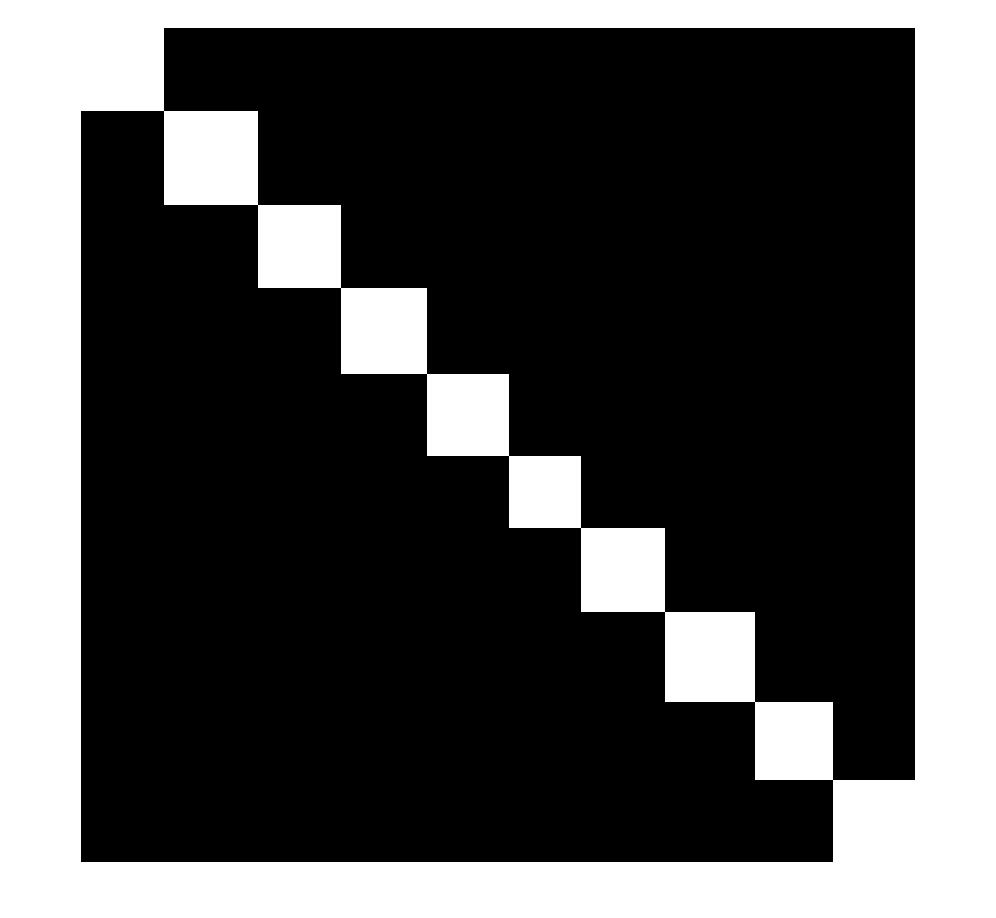
\includegraphics[width=0.3\textwidth]{chap2/k1.jpg}}
	\hspace{1em}
	\bisubcaptionbox{$k=100$下的热力核相似性矩阵}%
					{Affinity matrix of heat kernel with $k=100$}
					[0.3\textwidth]{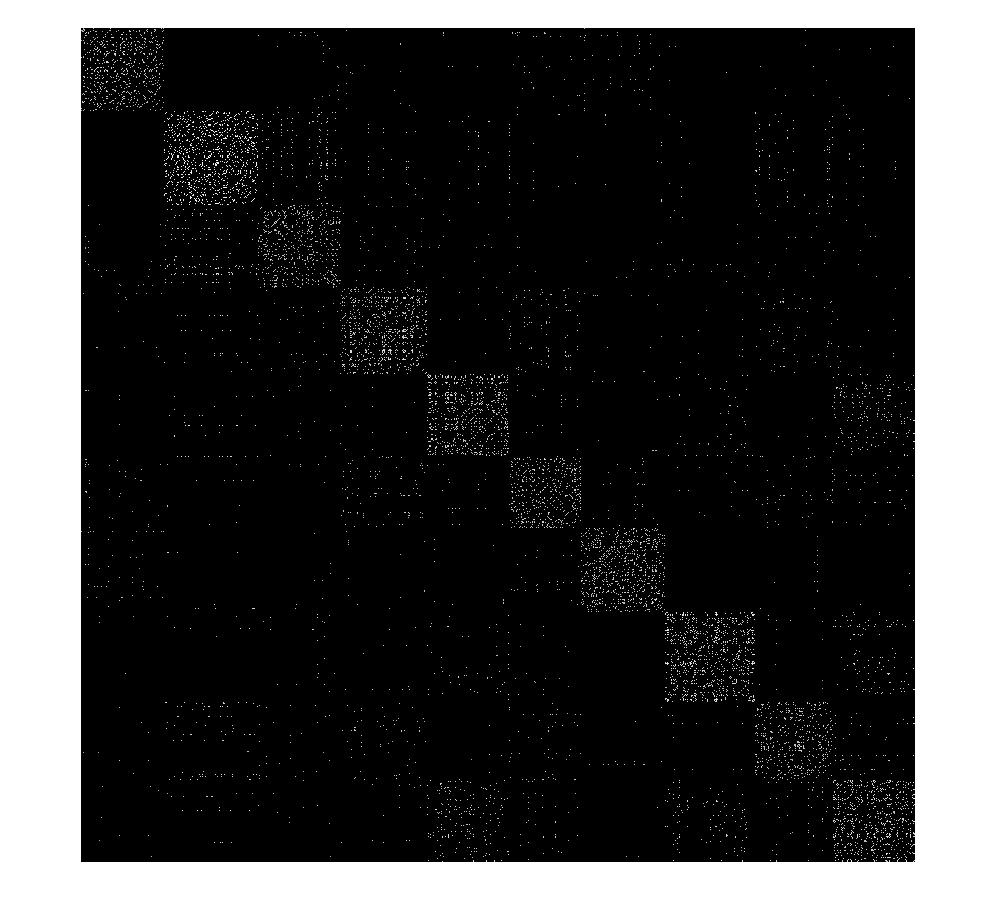
\includegraphics[width=0.3\textwidth]{chap2/k100.jpg}}
	\hspace{1em}
	\bisubcaptionbox{$k=1000$下的热力核相似性矩阵}%
					{Affinity matrix of heat kernel with $k=1000$}%
					[0.3\textwidth]{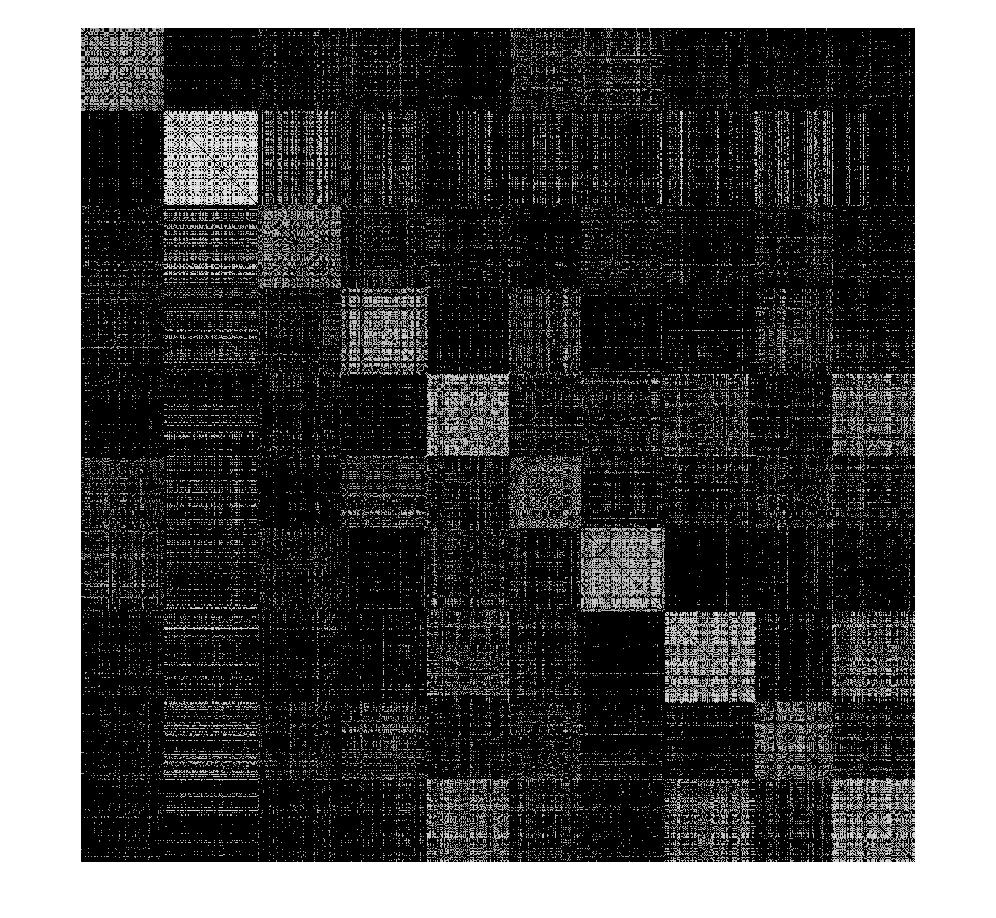
\includegraphics[width=0.3\textwidth]{chap2/k1000.jpg}}
	\bicaption{MNIST子集在理想情况及不同近邻数量$k$下的相似性矩阵}
			  {Ideal affinity matrix and affinity matrices with different neighborhood size $k$ on a subset of MNIST}
  	\label{fig2:affMat}
\end{figure}

本章所提出的方法的目标在于,针对谱聚类的线性近似,在最小的时间消耗下,提取更具有自适应性的相似性信息。这类信息将会更多的考虑局部性保持(locality preserving)这个优化目标,而不仅仅是图像间的距离。受到可扩展谱聚类和数据相似性学习方向上的研究成果\cite{chen2011large,nie2014clustering}的启发,本章提出了一个新颖的自适应相似性矩阵(Adaptive Affinity Matrix,AdaAM)方法。该方法的相似性矩阵相对稠密并可以同时捕捉到全局及局部信息。特别地,AdaAM将相似性矩阵分解成两个相同的低秩矩阵的乘积。作为文献\parencite{ng2002spectral}中描述的理想情况,如果我们假设同一个类内的点对相似性极为相似,则相似性矩阵可能会形成一个低秩矩阵。本算法采用与谱聚类方法相似的优化方法对分解后的矩阵进行优化求解。优化得到的相似性图作为最终结果前的中间态相似性矩阵。通过合并基于热力核获得的$k$-NN相似性图和中间态相似性矩阵,AdaAM采用朴素的谱聚类求解方法计算出一个最终的自适应相似性矩阵。我们将LPP方法作用于此特定的相似性矩阵上进行数据投影,以获得一个用于聚类的距离度量。

在本章中,我们将通过在图像数据集上的聚类实验展示所提出方法的有效性和高效性。第 \ref{sec2:Exp}节通过对本章提出的算法和基于$k$-NN的拉普拉斯特征映\cite{belkin2001laplacian}以及其他最先进方法进行对比展现了AdaAM方法在具有挑战性的数据集上的聚类效果具有明显优势。


\section{自适应相似性矩阵}
在本节中,我们首先对本节采用的数学符号进行说明,其次介绍中间态相似性矩阵的计算方法,然后描述最终自适应相似性矩阵的获取方式,最后对算法流程中的稀疏化策略进行介绍。
\subsection{符号说明}
在本章中,我们以大写英文或希腊字母代表矩阵,小写字母代表向量。所有元素全部为$1$的向量用$\bf{1}$表示。$H$表示中心化矩阵(centering matrix),其定义为:$H = I-\frac{1}{n}\bf{1}\bf{1}^T$。原始数据矩阵以$X \in \mathbb{R}^{n\times d}$表示,其中$n$为数据点的数量,$d$为数据维数。本章中将假设数据矩阵$X$为零均值列归一化矩阵,即$X = HX$。符号$x_i$表示数据矩阵$X$中的第$i$个数据点向量。我们用$A$表示线性投影,相应的距离度量矩阵表示为$M = A^TA$。因此,在该度量矩阵下的距离定义为$dis_m(x_i, x_j) = (x_i - x_j)^TM(x_i - x_j)$。我们将$k$-NN热力核矩阵表示为$W \in \mathbb{R}^{n \times n}$:
\begin{equation}
	w_{ij} = \begin{cases} \mathrm{exp}(-\frac{\|x_i-x_j\|_{2}}{t}), \; &x_i\in\mathcal{N}_k(x_j)\;\mathrm{or}\; x_j\in\mathcal{N}_k(x_i);\\
		0, &\mathrm{otherwise.}\end{cases}          
\end{equation}
此处,$\mathcal{N}_k(x)$表示数据点$x$的 $k$ 个最近邻的集合,我们延续了文献\parencite{niyogi2004locality}中对时间参数$t$的设定。相应的拉普拉斯矩阵表示为$L=D-W$,其中$D$为对角权重矩阵:$d_{ii} = \sum_j w_{ij}$。我们对中间态增量矩阵及最终自适应相似性矩阵都采用$\Delta$表示,相应的对角权重矩阵和拉普拉斯矩阵分别表示为$D_\Delta$和$L_\Delta = D_\Delta-\Delta$。

\subsection{中间态相似性矩阵}
我们将提出的AdaAM算法分为两个部分,分别是中间态相似性矩阵和最终自适应相似性矩阵。本节将对其中的中间态相似性矩阵部分的生成进行介绍。对于第$i$个数据点$x_i$,我们使用相似度$\delta_{ij}$对任意的数据点$x_i$和数据点$x_j$进行连接。由于希望任意两个数据点之间较近的欧氏距离能导致较大的数据点相似度,我们的目标为通过选择最优的相似度$\delta_{ij}$在特定合适的约束下最小化下述的目标函数,
\begin{equation}
	\mathop{\mathrm{min}} \sum_{i,j}^{n} \|x_i-x_j\|_2^2\;\delta_{ij},
\end{equation}
在这里,$\delta_{ij}$表示中间态相似性矩阵$\Delta$中第$ij$个元素。

不同于PCAN算法\cite{nie2014clustering},我们基于图拉普拉斯对该目标函数公式在其约束条件下进行变形,
\begin{equation}
	\mathop{\mathrm{min}}\; tr(X^TL_\Delta X).
	\label{eq2:Delta}
\end{equation}

由于在通常情况下图拉普拉斯为半正定矩阵,因此一个直接又看似可行的思路是将拉普拉斯矩阵分解为两个相同矩阵的乘积。在下文中我们将论述该思路不适用于我们的计算框架。

我们采用$U\in \mathbb{R}^{n\times s}$ 表示一个列正交矩阵,以满足$U^TU = I$,则我们可以假设
\begin{equation}
	L_\Delta = UU^T.
\end{equation}
在对原优化问题进行约束松弛的情况下,我们最终需要求解问题为:
\begin{equation}
	% \begin{split}
		U = \mathop{\mathrm{arg\;min}}_{U^TU=I}\; tr(X^TUU^TX) 
		\Rightarrow U = \mathop{\mathrm{arg\;min}}_{U^TU=I} \;tr(U^TXX^TU)
	% \end{split}
	\label{eq2:simpEigmap}
\end{equation}

如果我们假设矩阵$X$的乘积为矩阵$K$,即$K = XX^T$,则公式(\ref{eq2:simpEigmap})所得为一个简单形式的拉普拉斯特征映射\cite{belkin2001laplacian}。
由此,该优化问题可以通过选择矩阵$K$的多个最小特征值所对应的特征向量形成矩阵进行求解。但是,由于$K$为一个低秩矩阵,一般情况下满足条件$d\ll n$,$K$可以最小化公式(\ref{eq2:simpEigmap})中目标函数的特征向量都存在于数据矩阵$X$的零空间中。
因此,上述问题的最优解不唯一。受LSC(Landmark-based Spectral Clustering)算法\cite{chen2011large}启发,我们将相似性矩阵假设为一个半正定矩阵。不同于对拉普拉斯矩阵进行分解,我们将半正定的相似性矩阵分解为列正交矩阵 $P\in \mathbb{R}^{n\times r}$及其转置矩阵$P^T$的乘积,其中 $r$ 为预期下的矩阵$\Delta$的秩。

由此,我们可以将公式(\ref{eq2:Delta})改写为
\begin{equation}
	% 	\begin{split}
	% 		&\mathop{\mathrm{min}}_{P^TP=I} tr(X^T(D_\Delta-PP^T)X) \\
	% 		&\Rightarrow 
	\mathop{\mathrm{min}}_{P^TP=I} tr(X^TD_\Delta X)+tr(X^T(-PP^T)X),
	% 	\end{split}
	\label{eq2:XLX}
\end{equation}
此处,我们舍弃了连接权重为非负相似度以及图拉普拉斯为半正定矩阵这两个特性。相似性矩阵$\Delta$中的负值连接权重可以用于度量数据点间的不相似度。下面,我们将证明此优化问题的最优解将使$D_\Delta$ 等于 $\bf0$。

\begin{proposition}
	\label{thm2}
	在数据矩阵$X$为列归一化矩阵的条件下,最优化问题(\ref{eq2:XLX})的最优解$P$将使得$D_\Delta=\bf0$成立。
\end{proposition}

\begin{proof}
对于公式(\ref{eq2:XLX})中的第一部分,我们可以将其写为
\begin{equation}
	\begin{split}
		\mathop{\mathrm{min}}\;&\sum_{i=1}^{n} \|x_i\|_2^2\;d_{\Delta ii},\\
		s.t. \;\; &P^TP=I;\\
		&d_{\Delta ii}=(PP^T\textbf{1})_i.
	\end{split}
	\label{eq2:XD}
\end{equation}

令$z=(\|x_1\|_2^2, \|x_2\|_2^2, ... , \|x_n\|_2^2)^T$。此处,取拉格朗日乘子为$\lambda$,公式(\ref{eq2:XD})在一维情况下的优化问题可以表示为
\begin{equation}
	\mathop{\mathrm{min}}\; z^Tpp^T\textbf{1}-\lambda (p^Tp-1)
\end{equation}

最终,最小化优化问题(\ref{eq2:XD})可以被化简为求解问题
\begin{equation}
	\textbf{1}z^Tp=\lambda p
\end{equation}
中最小特征值对应地特征向量。因为矩阵$\textbf{1}z^T$为秩$1$矩阵,所以只存在一个非零特征值$\sum_{i=1}^{n}\|x_i\|_2^2$,同时这也意味着 $\lambda = 0$。由此可知,对于具有任意的小于 $n$的列数且满足优化问题(\ref{eq2:XD})的列正交矩阵$P$,我们可以得出$z^TPP^T\textbf{1}=0$。这个结论等价于
\begin{equation}
	\sum_{i=1}^{n} \|x_i\|_2^2\;d_{\Delta ii} = 0.
\end{equation}

一般性地,对于真实世界数据集中数据点$x_i$,$\|x_i\|_2^2\neq0$恒成立,故能够最小化目标函数(\ref{eq2:XLX})第一部分的最优解$P$ 具有性质$D_\Delta = \textbf{0}$。同时可知,具有性质$D_\Delta = \textbf{0}$的所有$P$的集合构成优化问题(\ref{eq2:XD})的解集。

最小化优化目标函数(\ref{eq2:XLX})的第二部分的矩阵$P$,可以通过求解下述特征问题中最大特征值获得:
\begin{equation}
	\begin{split}
		(XX^T)p = \lambda p
		\Rightarrow {\bf1}XX^Tp = \lambda {\bf1}p
	\end{split}
	\label{eq2:Solu}
\end{equation}

由数据矩阵$X$为零均值列归一化矩阵,可以得知$\lambda {\bf1}p = {\bf1}XX^Tp = 0$。因而,对于大于$0$的最大特征值,其对应地特征向量$p$总满足${\bf1}p = 0$。将令公式(\ref{eq2:XLX})中第二部分取得最小值的解$P$写为 $P=(p_1,p_2,...,p_t)$,可以得到
\begin{equation}
	%\begin{split}
	{\bf1}^T P = {\bf0} \Rightarrow {\bf1}^T PP^T = {\bf0} \Rightarrow d_{\Delta ii} = 0. %\quad(i=1,...,n)
	%\end{split}
\end{equation}
由此可知,特性$D_\Delta = \textbf{0}$对于公式(\ref{eq2:XLX})第二部分的最优解恒成立,并且该最优解属于公式(\ref{eq2:XD})的解集。所以,公式(\ref{eq2:XLX})第二部分的最优解同时可以使目标函数(\ref{eq2:XD})达到最优。完整的优化问题(\ref{eq2:XLX})的最优解使得
\begin{equation}
	D_\Delta={\bf0}。
\end{equation}
\end{proof}

由命题\ref{thm2}可知,优化目标函数(\ref{eq2:XLX})可以进一步化简为
\begin{equation}
	P=\mathop{\mathrm{arg\;max}}_{P^TP=I} \;tr(P^TXX^TP).
	\label{eq2:PXXP}
\end{equation}
公式(\ref{eq2:PXXP})的最优解可以通过对数据矩阵 $X$ 的奇异值分解求得,其运算复杂度依赖于数据维度$d$而不是数据量$n$。至此,我们从同时具有相似度和不相似度信息的原始数据分布中获得了中间态相似性矩阵 $\Delta = PP^T$。矩阵$\Delta$所对应的图拉普拉斯矩阵为$L_\Delta = D_\Delta-\Delta =-\Delta $。

为了能够缓解计算中的噪声影响以及矩阵秩减少的问题,我对矩阵$\Delta$进行了稀疏化处理。我们将在第\ref{sec2:sparse}节对稀疏化处理的细节进行进一步讨论。

\subsection{最终自适应相似性矩阵}
在本节中,我们对朴素的线性谱聚类进行公式化,并且给出最终自适应相似性矩阵的求解方法。

在已经求得中间态相似性矩阵$\Delta$的情况下,我们可以通过求解下述问题获得一个线性投影矩阵$A$:
\begin{equation}
	a = \mathop{\mathrm{arg\;min}}_{a^Ta=1}\; tr(a^TX^T(L+L_\Delta)Xa),
	\label{eq2:AXLXA}
\end{equation}
此处,$a$ 为矩阵$A$的一维情况,且$L+L_\Delta$是$k$-NN热力核与中间态相似性矩阵的拉普拉斯矩阵的组合。投影向量$a$可通过求解特征分解问题的最小特征值得到:
\begin{equation}
	X^T(L-\Delta)Xa = \lambda a
\end{equation}

然后,为在给定$A$的情况下求解公式(\ref{eq2:AXLXA})中的$L_\Delta$,我们依照对公式(\ref{eq2:XLX})的变形,将相似性优化问题进行重写并引入线性投影矩阵$A$:
\begin{equation}
	% \begin{split}		
		P = \mathop{\mathrm{arg\;min}}_{P^TP=I}\; \Big( c+tr(A^TX^TD_\Delta XA) 
		+tr(A^TX^T(-PP^T)XA)\Big),
	% \end{split}
	\label{eq2:AXDXA-PXAAXP}
\end{equation}
这里$c=tr(A^TX^TLXA)$,并且我们假设最终自适应相似性矩阵为$\Delta = PP^T$。由于$X$为列零均值的列归一化矩阵,则$XA$同样为列零均值矩阵,特性$D_\Delta = \textbf{0}$依然成立。由此可知,公式(\ref{eq2:AXDXA-PXAAXP})可化简为
\begin{equation}
	P = \mathop{\mathrm{arg\;max}}_{P^TP=I}\; tr(P^TXAA^TX^TP)
	\label{eq2:PXAAXP}
\end{equation}

公式(\ref{eq2:PXAAXP})可以通过对矩阵$A$进行奇异值分解并提取前$r$个最大奇异值对应的左奇异向量(left-singular vectors)进行求解。我们对从公式(\ref{eq2:PXAAXP})求解得到的自适应相似性矩阵$\Delta=PP^T$进行稀疏化处理,由此可以得到稀疏相似性矩阵。

直观来说,我们可以通过对公式(\ref{eq2:AXLXA})和公式(\ref{eq2:PXAAXP})进行交替迭代求解以使目标函数最小化。然而,如图\ref{fig2:itera}所示,在实际计算中,仅在执行一次迭代运算后所得到的自适应相似性矩阵即可取得很好的聚类效果。持续的迭代求解并没有表现出显著的聚类准确率提升。

在一些算法中图节点的权重具有重要作用,同时例如LPP的一类基于归一化割(Normalized Cuts,NCuts)的方法存在依赖于矩阵$D_\Delta$的优化约束条件。然而在我们的算法中有$D_\Delta = \textbf{0}$,因此,我们将由原始$k$-NN热力核计算得到的权重矩阵$D$叠加到求得的自适应相似性矩阵上,以还原损失的权重信息。最后,我们将原LPP算法中的相似性矩阵替换为由AdaAM方法求得的矩阵$\Delta+D$即可求解出线性投影矩阵$A$ 以及距离度量矩阵$M = A^TA$。

\begin{figure}[t]
	\centering
	\begin{subfigure}{0.49\textwidth}
		\centering
		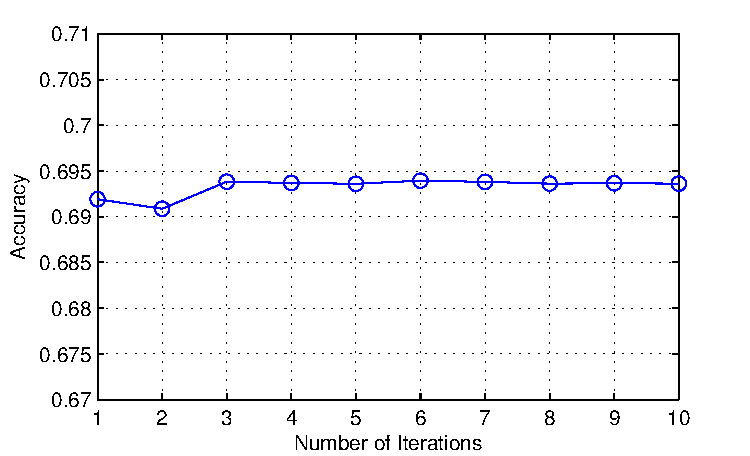
\includegraphics[width=\textwidth]{chap2/itera_data.pdf}
		\caption{}
		\label{fig2:itera}
	\end{subfigure}
	% \hspace{1em}
	\begin{subfigure}{0.49\textwidth}
		\centering
		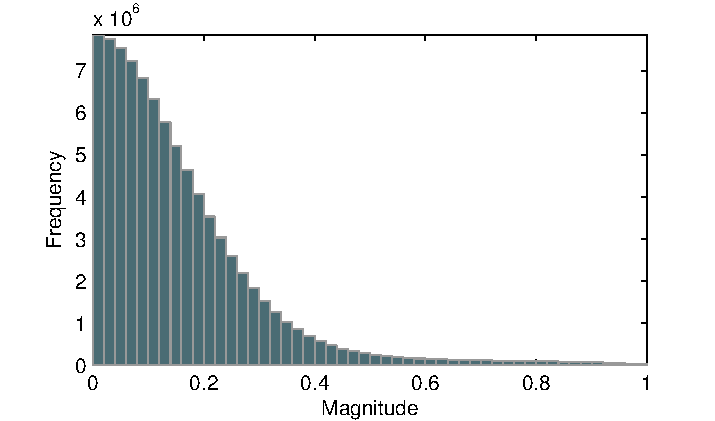
\includegraphics[width=\textwidth]{chap2/delta_hist.pdf}
		\caption{}
		\label{fig2:Hist}
	\end{subfigure}
	\bicaption{a)在数据集USPS上不同的迭代计算次数的聚类效果评价结果。迭代计算所贡献的精度提升小于0.5\%;b)数据集USPS的最终自适应相似性矩阵的元素强度直方图}
			  {a)The evaluation of the clustering performance with different times iterative computation on the data set USPS. The contribution to accuracy made by iteration is less than 0.5\%. b)The histogram of the element magnitude of the final adaptive affinity matrix obtained from data set USPS. }
\end{figure}

\subsection{稀疏化策略}
\label{sec2:sparse}

从优化问题(\ref{eq2:PXXP})和(\ref{eq2:PXAAXP})我们可以观察到,矩阵$XX^T$ 和 $XAA^TX^T$都是低秩矩阵。由于上述的优化问题都需要通过矩阵奇异值分解进行求解,所以这个低秩现象将会导致最优解矩阵$P$的列的数量远小于矩阵 $XX^T$ 和 $XAA^TX^T$ 的秩数。这个计算流程将会产生低秩的相似性矩阵,而低秩相似性矩阵会导致我们的算法中的矩阵秩的进一步减小。为避免该矩阵秩持续减小问题的发生,我们在提出的算法中对矩阵实施了稀疏化操作。我们采用的稀疏化策略可以同时缓解数据图中的噪声边问题。

在图\ref{fig2:Hist}中,我们展示了不经过稀疏化处理情况下通过公式(\ref{eq2:PXAAXP})求得的自适应相似性矩阵的元素强度直方图。从图\ref{fig2:Hist}中我们可以观察到,绝大多数的相似性矩阵元素都集中在数值强度较小的范围内,这有效证明了我们对相似性矩阵进行稀疏化处理的合理性。同时,稀疏化处理可以有效的保留住一部分表达能力更强的相似性元素。

受到$k$-NN热力核构造思路的启发,我们对相似性矩阵$\Delta$中的全部元素根据强度大小进行降序排序,只保留其中的前$s$个元素。假设在稀疏化处理后,仅有类内数据点间的相似性被保留下来,不同类间的数据点相似性被删除。在这种情况下,我们考虑到参数$s$的大小应该与聚类的类数成反比,这可以使最终保留下来元素数量近似与图\ref{fig2:affMat}中所示的理想情况下元素数量保持固定比例。参数$s$的计算公式为:
\begin{equation}
	s = \lfloor \frac{n^2}{\alpha c}\rfloor
\end{equation}
此处 $\lfloor \cdot\rfloor$为向下取整函数,$n^2$为矩阵$\Delta$中的元素总数量,$c$为聚类的类数,$\alpha$为一个可调的比例系数。

\begin{algorithm}[t]
	\SetKwInput{KwData}{输入}
	\SetKwInput{KwResult}{输出}
	\caption{自适应相似性矩阵}
	\label{alg2:AdaAM}
	\KwData{数据点 $X \in \mathbb{R}^{n \times d}$;聚类数量 $c$;近邻数量 $k$;降维后维度 $m$。}
	\KwResult{距离度量矩阵 $M$ 和线性投影矩阵$A$。}
	构建$k$-NN热力核矩阵$W$,相应的对角化权重矩阵$D$ 以及拉普拉斯矩阵$L$。\\
	根据公式(\ref{eq2:PXXP}),计算获得列正交矩阵$P$,并求得相应的中间态相似性矩阵$\Delta = PP^T$。\\
	根据公式(\ref{eq2:AXLXA}),求解得到线性投影矩阵$A$。\\
	求解公式(\ref{eq2:PXAAXP}),构造新的$P$矩阵,生成相应的最终自适应相似性矩阵$\Delta = PP^T$。\\
	通过将LPP算法作用于相似性矩阵$\Delta + D$,计算出线性投影矩阵 $A\in\mathbb{R}^{m\times d}$ 及距离度量矩阵 $M=A^TA$。
\end{algorithm}

对于计算中间态相似性矩阵中的第一次稀疏化处理,我们设置$\alpha$为$2.5$,对于计算最终自适应相似性矩阵中的第二次稀疏化,我们将$\alpha$设置为$5$。此处的$\alpha$通过参数搜索确定,并且能够在大多数数据集上给出稳定的表现。

我们在算法\ref{alg2:AdaAM}中对我们所提出的AdaAM算法流程进行了总结。我们在算法实现中将降维后的维度$m$设置为与聚类的类数相同。


\section{实验结果}
\label{sec2:Exp}
在本节中,我们针对所提出算法在图像数据集上的聚类效果、对构建相似性图中的近邻数量敏感性以及算法的运行时间设计了大量的实验,并与其他最先进的算法进行的对比。实验结果验证了所提出的AdaAM算法的有效性、稳定性和高效性。
\subsection{数据集描述}
我们在五个被广泛使用的灰度图像数据集上对所提出的算法及对照算法进行了性能评估:

\begin{figure}[t]
	\centering
	\bisubcaptionbox{UMIST数据集}%
					{UMIST dataset}
					[0.49\textwidth]{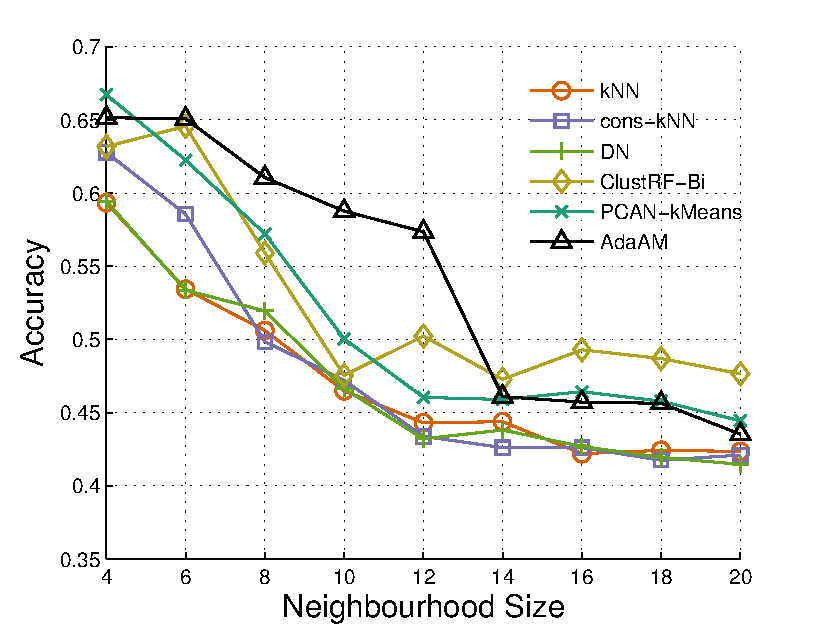
\includegraphics[width=0.49\textwidth]{chap2/sens_UMIST.pdf}}
	\bisubcaptionbox{COIL20数据集}%
					{COIL20 dataset}
					[0.49\textwidth]{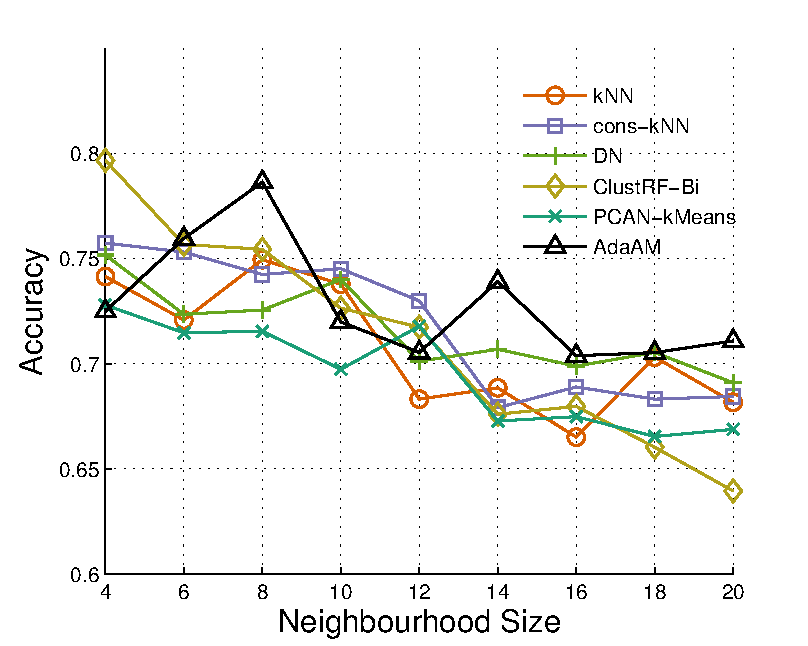
\includegraphics[width=0.49\textwidth]{chap2/sens_COIL20.pdf}}
	\bicaption{在数据集UMIST和COIL20上不同的近邻数量$k$的情况下的算法聚类效果比较}{Clustering results comparison between methods with different neighborhood size $k$ on UMIST and COIL20}
	\label{fig2:Sen}
\end{figure} 

\begin{itemize}
	\item {\textbf{UMIST}}。UMIST人脸数据集 \cite{graham1998characterising}包括20个人的共计575张灰度图片,每张图片尺寸为220$ \times $220像素。在我们的实验中,我们将原图缩小到40$ \times $40像素。
	\item {\textbf{COIL20}}。COIL20数据集\cite{nene1996columbia}包含20各不同物体,共1,440张灰度图片。数据集图片尺寸为32$\times$32像素,图片背景被丢弃仅保留了前景物体。
	\item {\textbf{USPS}}。USPS手写数字数据库\cite{hull1994database}包含了10个数字共计9,298张的灰度图像,图像尺寸为16$\times$16像素。
	\item {\textbf{MNIST}}。MNIST手写数字数据库\cite{lecun1998gradient}训练集包含10类数字共计70,000张灰度图像。图片尺寸为28$\times$28像素。在我们的实验中,我们使用了该数据库训练集中前10,000张图片。
	\item {\textbf{ExYaleB}}。Extended Yale Face Database B(ExYaleB)人脸数据集\cite{KCLee05}由2,414张经过裁剪的人脸图像组成,包含38个个体,每个个体在不同光照下拍摄大约64张图像。在实验中,我们将ExYaleB图像缩小到32$ \times $32像素。
\end{itemize}

在表格\ref{tab2:Data}中,我们总结了五个基准图像数据集的统计量描述。

\begin{table}[t]
	\bicaption{五个基准数据集的统计量描述}{Statistics of five benchmark data sets}
	\label{tab2:Data}
	\centering
		%\begin{sc}
	\begin{tabular}{l c c c}
		\toprule
		数据集 & 实例数目 & 特征维度 & 类别数目\\ 
		\midrule
		UMIST & 575 & 1,600 & 20\\
		COIL20 & 1,440 & 1,024 & 20\\
		USPS & 9,298 & 256 & 10\\
		MNIST & 10,000 & 784 & 10\\
		ExYaleB & 2,414 & 1,024 & 38\\
		\bottomrule
	\end{tabular}
		%\end{sc}
\end{table}

\subsection{对照算法介绍}
我们将所提出的AdaAM方法的聚类效果与本节中介绍的其他相似性学习算法进行了比较。 我们将LPP方法分别应用于通过这些最先进方法生成的相似性矩阵,以获取距离度量矩阵。

\begin{itemize}
	\item \textbf{Con-$k$NN}。Consensus $k$-NNs(Cons-$k$NN)算法\cite{premachandran2013consensus}的目标在于选取更鲁棒的数据点近邻集合。Cons-$k$NN方法通过收集多轮$k$-NN相似性计算中的共识信息,来为数据点近邻集合的选择提供判断标准。
	\item \textbf{DN}。Dominant Neighborhoods(DN)算法\cite{pavan2007dominant}通过在已构建出的相似性图中迭代地选取最大团的方法,实现对相似性矩阵中存在的噪声边的过滤。
	\item \textbf{ClustRF-Bi}。ClustRF-Bi算法\cite{criminisi2012decision,pei2013unsupervised}是ClustRF-Strct \cite{zhu2014constructing}算法的一个计算量较小的特例。由于原始ClustRF-Strct算法在仅有数千个数据实例的情况就需要极大量的计算机内存,我们在本章的实验中采用了这个计算量和内存需求相对可行的特例。ClustRF-Strct提出了一种具有结构感知能力的相似性推断模型,该模型通过利用随机森林进行聚类从而构建数据的相似性图。ClustRF-Bi作为一个特例仅通过随机森林聚类构建二值化的相似性矩阵。
	\item \textbf{PCAN}。文献\parencite{nie2014clustering}提出了Projected Clustering with Adaptive Neighbors(PCAN)方法。由于PCAN是一种可以同时生成线性投影和聚类的算法,所以在结果展示中,我们将PCAN的投影和$k$-means聚类的组合方法表示为PCAN-$k$Means方法,并在表格\ref{tab2:Acc}中显示仅采用PCAN算法生成的聚类结果以供对照参考。
	\item \textbf{$k$-NN}。我们还将所提出的方法与采用$k$-NN热力核相似性矩阵直接进行线性投影的效果进行比较,即采用$k$-NN热力核的LPP算法。我们在后续实验中使用$k$-NN表示这种典型的方法。
\end{itemize}

\begin{figure}[t]
	\centering
	\bisubcaptionbox{USPS数据集}%
					{USPS dataset}
					[0.49\textwidth]{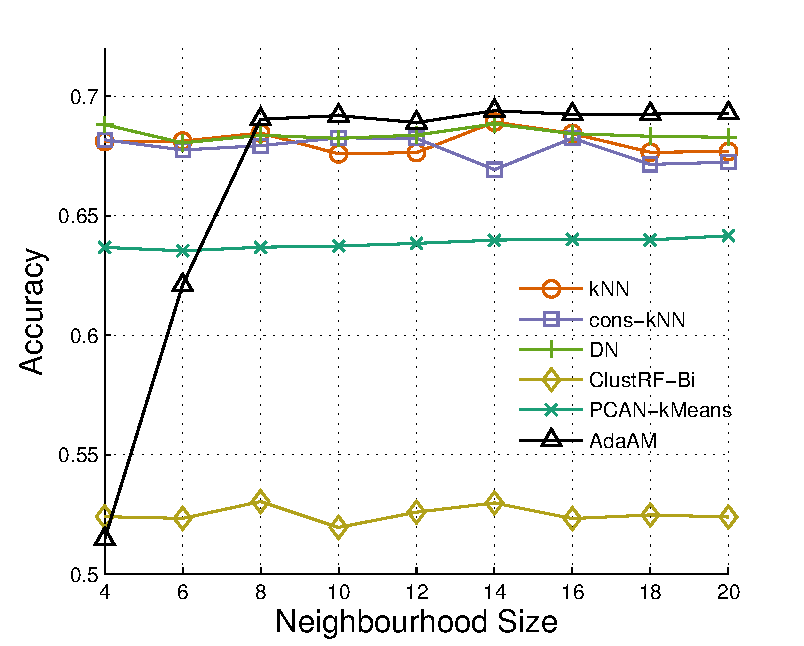
\includegraphics[width=0.49\textwidth]{chap2/sens_USPS.pdf}}
	\bisubcaptionbox{MNIST数据集}%
					{MNIST dataset}
					[0.49\textwidth]{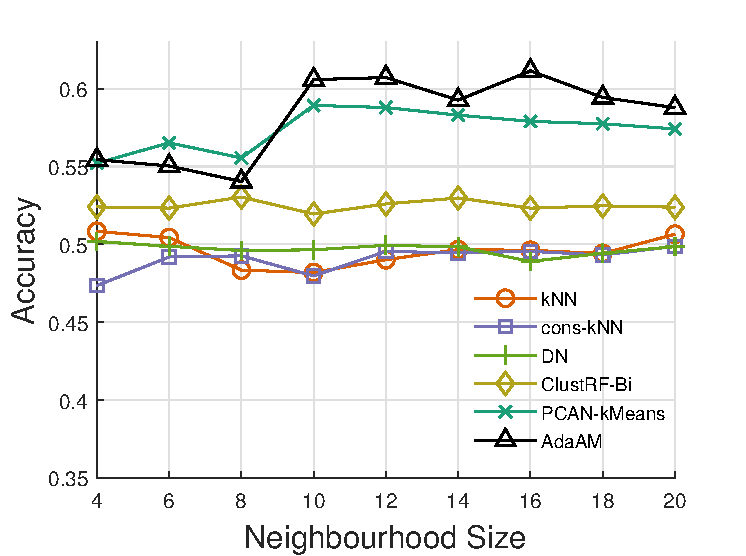
\includegraphics[width=0.49\textwidth]{chap2/sens_MNIST.pdf}}
	\bicaption{在数据集USPS和MNIST上不同的近邻数量$k$的情况下的算法聚类效果比较}{Clustering results comparison between methods with different neighborhood size $k$ on USPS and MNIST}
	\label{fig2:Sen2}
\end{figure} 
\begin{table}[t]
	\bicaption{不同图像数据集上的聚类准确率(\%)}
	{Clustering accuracy on different image datasets(\%)}
	\label{tab2:Acc}
	\centering
	% \begin{small}
		%\begin{sc}
		\begin{tabular}{llccccccc}
			\toprule
			& &$k$-NN &Cons-$k$NN &DN &ClustRF-Bi &PCAN-$k$Means &PCAN& AdaAM
			\\
			\midrule
			\multirow{2}{*}{UMIST} & Avg & 58.16& 60.27& 59.15& 64.63& 53.79& \multirow{2}{*}{55.30}   & \textbf{66.06}\\
			& Max& 65.39& 69.22& 66.96& 74.44& 56.52&& \textbf{75.65}\\
			\midrule
			\multirow{2}{*}{COIL20} & Avg & 71.89& 75.53& 71.95& \textbf{76.50}& 72.28& \multirow{2}{*}{81.74}& 74.72\\
			& Max& 81.18& 84.31& 82.01& 85.07& 83.75&& \textbf{87.29}\\
			\midrule
			\multirow{2}{*}{USPS}  & Avg & 68.25& 68.21& 68.08& 58.74& 64.04& \multirow{2}{*}{64.20}  & \textbf{69.36}\\
			& Max& 68.35& 68.34& 68.31& 65.90& 67.95&& \textbf{69.61}\\
			\midrule
			\multirow{2}{*}{MNIST} & Avg & 48.13& 47.88& 49.72& 51.93& 58.93& \multirow{2}{*}{59.83}  & \textbf{60.84}\\
			& Max& 48.27& 48.00& 49.76& 52.03& 58.98&& \textbf{61.34}\\
			\midrule
			\multirow{2}{*}{ExYaleB} & Avg& 24.17& 25.63& 24.21& 23.10& 25.74& \multirow{2}{*}{25.89} & \textbf{54.36}\\
			& Max& 26.76& 28.75& 27.42& 26.43& 27.63&& \textbf{57.87}\\
			\bottomrule
		\end{tabular}
		%\end{sc}
	% \end{small}
\end{table}

\subsection{参数选择与实验设置}
由于在无监督学习任务中不存在验证数据集,所以为了实现更一般化的参数选择情况,我们对实验中的所有算法采用了相同的参数选择标准。我们将每个数据实例的近邻数量设置为$k = \mathrm{Round}(\mathrm{log}_2\frac{n}{c})$,其中$n$为数据实例数量,$c$为类别数量,$Round(x)=\lfloor x+\frac{1}{2}\rfloor$。我们参考文献\parencite{ng2002spectral}的结论,将投影的维度设置为与类别数目相同,即距离度量矩阵的秩与类别数相同。所提出的算法中的其他参数在所有实验中均固定不变。

我们将10次独立重复的$k$-means聚类表示为1轮聚类,并在每轮所有结果中选择类内和最小的结果作为该轮$k$-means的聚类结果。在进行聚类性能评估中,我们对每种算法分别应用100轮$k$-means聚类用于(参见表\ref{tab2:Acc})。在近邻数量$k$的敏感性实验中,我们应用10轮$k$-means聚类(参见图\ref{fig2:Sen},图\ref{fig2:Sen2}和图\ref{fig2:Sen3}),而在运行时间测试实验中,我们仅进行一轮$k$-means聚类(参见图\ref{fig2:Time})。


\begin{figure}[t]
	\centering
	\bisubcaptionbox{ExYaleB数据集}%
					{ExYaleB dataset}
					[0.9\textwidth]{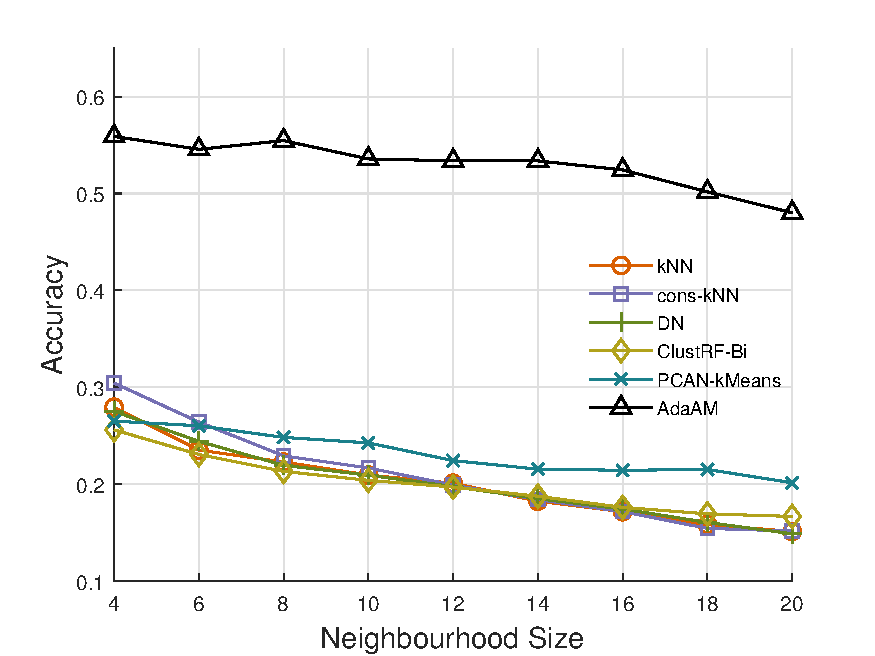
\includegraphics[width=0.9\textwidth]{chap2/sens_ExYaleB1.pdf}}
	\bicaption{在数据集ExYaleB上不同的近邻数量$k$的情况下的算法聚类效果比较}{Clustering results comparison between methods with different neighborhood size $k$ on ExYaleB}
	\label{fig2:Sen3}
\end{figure} 
在聚类效果评估中,我们通过将获得的聚类标签与数据集的真实标注进行比较,使用准确率(accuracy,Acc)来衡量性能。准确率定义如下:
\begin{equation}
	\mathrm{Acc} = \frac{1}{n}\sum^{n}_{i=1}\delta(p_i, map(q_i))
\end{equation}
其中$n$为数据实例数量,$p_i$是数据$x_i$的预测标签,$q_i$为真实标签。当$x=y$时$\delta(x, y) = 1$,否则$\delta(x,y) = 0$。$map(q_i)$表示最佳匹配函数,该函数通过在预测出的类之间交换类标签实现,预测标签与真实标签的最佳匹配。

全部实验都通过MATLAB R2014a实现,并运行在具有Quad Core 3.00 GHz CPU和16 GB内存的Linux系统计算机上。

\subsection{性能评估与比较}
\begin{figure}[t]
	\centering
	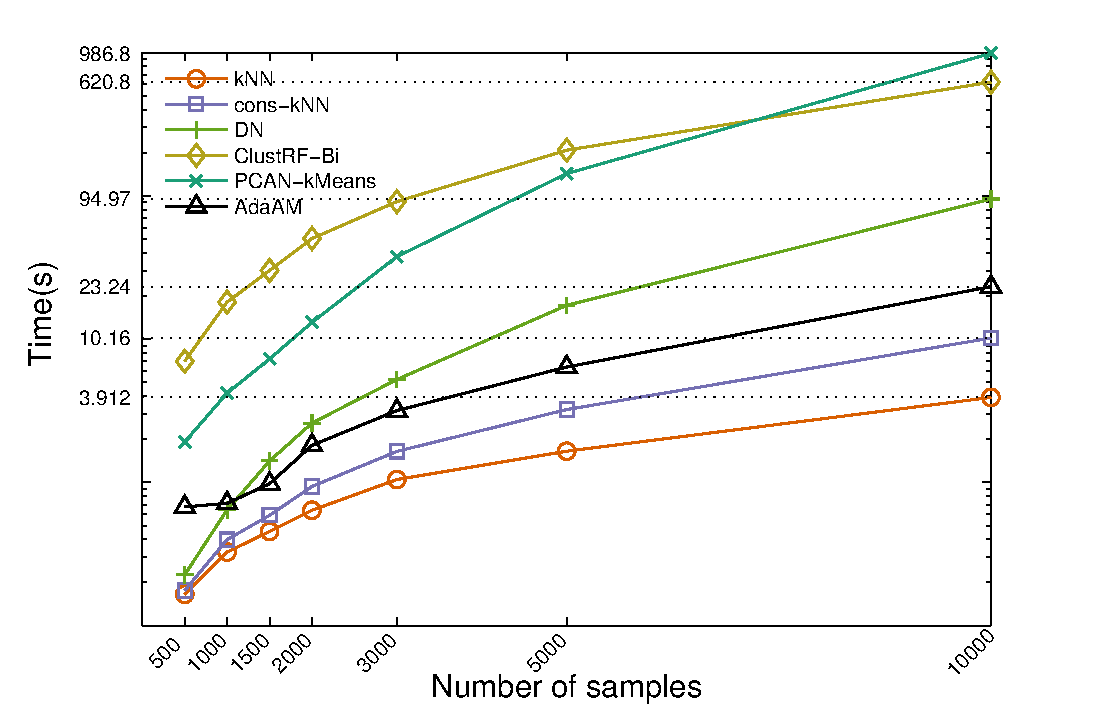
\includegraphics[width=0.9\columnwidth]{chap2/time.pdf}
	\bicaption{不同数据实例数量的情况下六个算法的时间使用比较}{Time consumption of six approaches with different number of data instances}
	\label{fig2:Time}
\end{figure}

在聚类准确率评估的实验中,我们在上述五个基准数据集上对提出的AdaAM方法及其他五种算法进行了数据投影效果的评估。表\ref{tab2:Acc}给出每个模型在100轮$k$-means聚类中聚类预测准确率的平均值和最大值。由于PCAN算法不通过$k$-means聚类而直接产生聚类结果,所有PCAN性能评估结果仅有唯一结果,不存在平均值与最大值。从表\ref{tab2:Acc}中我们可以观察到AdaAM算法在无监督度量学习任务上的优越性。在绝大多数情况下,AdaAM算法的性能明显优于其他方法。我们的方法在五个数据集的平均准确率指标上获得了四个最优,在最大准确率指标上五个全部最优。我们还可以观察到,所提出的AdaAM在ExYaleB数据集上相对其他五种方法具有绝对性优势。与其他数据集不同,ExYaleB中的图像数据已针对人脸进行了较好地对齐,并图片拍摄场景处于不同的光照环境下。这种差异使得相同光照下的图片即使属于不同类别的图像依然具有较大的相似度,从而使数据图上类间连接增多,导致了高秩的相似性矩阵。我们的方法基于最优相似性矩阵的低秩近似,能够有效处理相似性矩阵中的此类噪声。

由于在准确率评估实验中近邻数量$k$选择标准是固定的,这可能会导致算法无法在实验中获得最优性能。因此我们在图\ref{fig2:Sen}、图\ref{fig2:Sen2}及图\ref{fig2:Sen3}中展示了AdaAM与对照算法在五个图像数据上的聚类准确率随近邻数量大小变化的趋势。我们在每个数据集上分别设计了近邻数量从$k=4$到$k=20$、间隔为2的9组实验,以评估不同算法的聚类效果是否会随近邻数量不同,即相似性矩阵的稀疏程度,而产生显著的波动。从图中可以看出,在大多数情况下,AdaAM可取得最佳性能,并且对近邻数量的敏感性与其他模型相当或更低。由于我们的方法基于最佳相似性矩阵的低秩近似,需要更多的成对相似度的信息。因此,对于极小的近邻数量$k$,部分基线方法有时比我们的方法效果更好,这一点可以从图\ref{fig2:Sen2}可以看出。

在图\ref{fig2:Time}中,我们通过半对数图描绘了六种算法在不同数据量的MNIST子集上的运行时间,以此说明AdaAM方法的高效性。 从图中可以看出,我们的方法在实际使用中是一种时间代价较低的算法。相比于PCAN-$k$Means,ClustRF-Bi和DN方法,AdaAM算法的时间消耗要低得多。需要注意的是,$k$-NN作为一个基线算法,本身并不需要进行相似性矩阵学习,因此其所需的运行时间仅包括$k$-NN热力核相似性矩阵构建、LPP线性投影矩阵计算及$k$-means聚类这三种所有对照算法共享的基本操作,所以其计算效率必然最高。我们同时还展示了AdaAM的运行时间大约为Cons-$k$NN的两倍,但整体性能性能要好得多。

\section{本章小结}
在本章中,我们提出了一种用于无监督度量学习的创新性的的相似性学习方法,称为自适应相似性矩阵矩阵(Adaptive Affinity Matrix,AdaAM)。在我们所提出的新的相似性学习模型中,相似性矩阵是从与谱聚类相同的计算框架中学习获得的。 更具体地说,我们表明相似性学习可以简化为奇异值分解问题。获得学习到的相似性矩阵后,可以借助于类似LPP这样基于相似性图的现成的算法来学习距离度量。我们所采用的低秩近似的优化方法可以在相似性矩阵学习的过程中进一步提高学习效率。
我们在UMIST、COIL20、USPS、MNIST及ExYaleB五个被广泛使用的图像数据集上对AdaAM及其他对照算法的进行了大量聚类实验。
实验结果证明了所提出的方法AdaAM的性能优越性、稳定性与高效性。
% !TEX root = ../thesis.tex
\chapter{基于相似性融合学习的多模态约束传播}
在前一章中,本文研究了无监督情况下的数据相似性学习方法。本章将研究具有成对约束信息的多模态环境下聚类任务中的相似性学习。多模态是对应于单模态的一个概念,多模态表示对于每个被观察物体,都通过不同方式或不同角度对目标物体进行观察,并产生多类不同的描述信息。而成对约束信息,是半监督约束聚类中的一个重要概念。
在约束聚类的任务中,两个对象是否属于同一聚类的信息通常由成对约束表示,表示两个数据是否有被观测到的必然联系,也称为必然连接(must-link)约束和必然不连接(cannot-link)约束。 成对约束是一种特别经济的辅助信息,尽管其不能提供任何有关类别的明确信息,但可以从用户端通过高效的交互方式进行信息采集。
本章针对多模态约束聚类这一应用问题,在多模态约束传播的框架下提出了特定的相似性学习方法,以使得在多模态问题环境下可以通过各模态内部相似性及约束信息学习生成统一的相似性矩阵。

\section{引言}
\label{sec3:intro} 
在过去的十几年的时间里,成对约束已广泛用于约束聚类和度量学习问题中。Wagstaff 等人首先在他们的工作中将成对约束引入聚类问题\cite{wagstaff2000clustering,wagstaff2001constrained}。Xing等人提出了一个具有成对约束的距离度量学习框架\cite{xing2002distance}。度量学习中的一些后续工作也证明了成对约束的作用\cite{weinberger2005distance,davis2007information}。

由于成对约束是一种特殊的弱监督信息,因此一些约束传播方法\cite{lu2008constrained,lu2010constrained,fu2011symmetric}陆续被提出以充分利用成对约束信息。Lu和Carreira-Perpinan在文献\parencite{lu2008constrained}中提出了Affinity Propagation(AP)算法,该算法通过借助高斯过程实现了约束传播。Lu和Ip在文献\parencite{lu2010constrained}中提出了Exhaustive and Efficient Constraint Propagation(E$^2$CP)方法。E$^2$CP算法在标签传播(label propagation)\cite{zhou2004learning}的学习框架下对成对约束信息进行传播,并且作者将约束信息的传播解释为半监督的二分类学习问题。作为能够有效利用辅助信息的一种有力工具,约束传播已经被广泛应用在半监督学习场景中。文献\parencite{jian2016interactive}提出了ACP Cut算法,以将用户所提供的交互式信息的特征传播到整个图像中,以用于个性化的图像分割。文献\parencite{han2016segmentation}提出了一种用于图像分割的高效的选择性约束传播方法,并且仅在图像的一个像素子集上执行约束传播。在实际应用中,由于观察到的真实信息数据的量很少,半监督学习方法经常会面临标注有缺陷的问题。Zhu等人设计了约束传播随机森林(Constraint Propagation Random Forest,COP-RF)算法\cite {zhu2016constrained},该方法不仅能够应对由于有缺陷的标注数据产生的噪声约束,而且能够执行有效的稀疏化约束传播。文献\parencite{wang2016semi}利用成对约束传播的方法来提升半监督的非负矩阵分解的效果。Wu等人采用约束传播方法在初始化的约束信息中扩展增加更多的有用信息,以用于在视频中进行人脸的聚类和跟踪\cite{wu2017coupled}。

上述提到的约束传播方法全部是针对单模态数据集提出的。事实上,我们经常需要分析具有多模态多视图的数据集,例如文本描述和多种类型的图像特征。近年来,多模态数据的融合学习非常普遍,并且在例如多传感器系统、生物医学研究和环境研究等许多领域中有深入研究。不同模态之间的关联将为数据本身引入一种新形式的多样性。这些存在于不同的模态之间的信息交互的现象带来了新的约束类型,这种约束可以减少相应学习过程中的自由度\cite{lahat2015multimodal}。Yu等人指出,具有视觉和用户点击特征的多模态距离度量学习可以改善检索中的图像排序效果\cite{yu2017deep}。文献\parencite{kahou2016emonets}提出了EmoNets方法用于视频中的情绪识别,该EmoNets可以学习多种专家模型,每种模型仅关注一种模态。Poria等人研究了情感计算(affective computing)中的多模态融合,并制定了一种多模态情感分析框架,以实现在视频内容和其他不同模态信息中提取用户的情绪\cite{poria2017review,poria2017ensemble}。Shen等人提出了一种多模态抑郁字典学习(Multimodal Depressive Dictionary Learning,MDL)\cite{shen2017depression}方法,通过利用社交媒体中的情绪特征、用户资料特征及话题级别特征等不同模态的特征信息,以进行抑郁症检测。此外,高度类似于多模态数据融合的多视图数据融合也被广泛应用于许多实际问题的研究中,例如面部识别\cite{kan2016multi}和动作识别\cite{shao2016kernelized}。

近几年,一些为解决多模态约束传播问题的方法被先后提出\cite{fu2011multi,fu2012modalities,lu2013unified,lu2013exhaustive}。但是,这种多模态约束传播方法中大多数都是为特殊情况而设计的,即只有两种不同的模态需要处理,例如Unified Constraint Propagation(UCP)\cite{lu2013unified}算法和Multi-Source Constraint Propagation(MSCP)\cite{lu2013exhaustive}算法。经验上,我们经常可能会需要能够处理两种以上模态的算法,而上述方法在这种情况下是不适用的。
尽管文献\parencite{fu2011multi}中提出的Multi-Modal Constraint Propagation(MMCP)方法对模态的数量没有限制,但是MMCP的学习需要有每种模态的先验知识作为数据输入。这意味着研究人员需要手动决定每种模态的重要性。当有数量比较多的模态需要处理时,这样的手动设置方案几乎是不可行的。但是,MMCP依然为多模态约束传播提供了一个通用的学习框架。文献\parencite{fu2012modalities}中提出的Multi-modal Constraint Propagation(MCMCP)方法在约束传播中引入了共识正则器,以迫使不同模态上的约束传播结果保持一致。

多模态学习中普遍存在的一个挑战是如何实现模态融合并有效利用多种数据模态所提供的额外信息。在本章中,我们将注意力集中在利用数据所提供的少量监督信息进行相似性矩阵的融合学习上。在多模态的标签传播问题中,监督信息是每个对象的标签,需要通过融合不同模态的相似性矩阵,以估计标签扩散的结果。然而在约束传播和标签传播之间有着一定的差异。在多模态约束传播问题中,监督信息和传播得到的结果都是相似性信息,这使得从这些不同模态的成对约束中融合出一个好的相似性矩阵变得更加直观且合理。 因此,可以考虑在融合学习中充分利用多模态数据集中的成对约束,同时实现约束的传播和相似性矩阵融合的学习。

在本章中,我们提出了一种新的用于约束传播的多模态融合学习方法(Multi-modal Fusion Learning,MFL)。MFL继承了MMCP方法所提出的多模态约束传播学习框架。我们首先将一种被广泛应用于多模态聚类和标签传播问题中的多模态融合方法引入到约束传播学习框架中,在本章中,该算法被视为基线方法。由于是通过从拉普拉斯正则化(Laplacian regularization)中学到的松弛后的权重系数构建此基线方法,因此该方法被称为松弛权重组合(Relaxed Weight Combination,RWC)。
实验结果表明,RWC方法所学习的融合结果可能会深陷入一些判别性较差的模态而忽视高判别性的模态。
受RWC方法的进一步启发,本章提出的MFL方法在约束传播的过程中同时从约束传播和拉普拉斯正则化这两个优化目标中学习多模态融合。从数据中观察到的成对约束可以提供少量的证据以判断一个模态的信息是否有高判别性。同时,拉普拉斯正则化可以确保具有更一致的相似性矩阵的模态将受到足够多的重视。所提出的MFL同时还可以作为模态选择器,MFL能够自动消除没有帮助的模态,并维护一个相对稀疏的候选模态列表。

\section{约束传播背景知识}
在本节中我们首先将针对多模态约束传播对所用到的数学符号在前一章的基础上进行补充说明,然后简要回顾典型的单模态约束传播算法E$^2$CP\cite{lu2010constrained}和多模态约束传播算法MMCP\cite{fu2011multi}。
\subsection{符号说明}
在下文中,矩阵将用大写字母表示,向量和标量以小写字母表示。给定矩阵$ {A} \in \mathbb{R}^{n\times m}$,$ a_{ij} $为矩阵$A$在位置$ i,j $的元素。相似地,$ \alpha_{i} $ 为向量 $ {\alpha} $的第 $ i $个元素。考虑到多模态的情况,在未特殊说明的情况下,在矩阵和向量中采用下标$s$区分多模态数据集不同的模态,即${A}_s$表示源自模态$s$中的一个矩阵。矩阵$ {A}_s $ 中的第$ i,j $个元素被表示为$a_{ij,s}$。
%$ \boldymbol{\alpha} $ 此外,对于矩阵$A$和矩阵$D$我们定义$ \|{A}\|_{D} = \mathrm{tr} ({A}^T{D}{A})^{\frac{1}{2}}$ 以保持文中公式的简洁。

我们用大写的花体字母表示集合和图。给定一个数据集合$\mathcal{X} = \{x_1,\dots,x_n \}$,每一个数据实例的数据被表示为$x_i$。$x_i$仅表示第$i$个数据实例本身,不代表任何数据向量或特征向量,更进一步地,将数据$x_i$在模态$s$上的数据特征向量表示为$x_{i,s}$。

对于第$s$个模态,可以在全部$n$个数据实例上通过$k$-NN热力核构建相似性矩阵$ {W}_s$:
\begin{equation}
w_{ij} = \begin{cases} \mathrm{exp}(-\frac{\|x_{i,s}-x_{j,s}\|_{2}}{t}), \; &x_{i,s}\in\mathcal{N}_k(x_{j,s})\;\mathrm{or}\; x_{j,s}\in\mathcal{N}_k(x_{i,s});\\
0,&\mathrm{otherwise,}\end{cases}   
\label{eq3:GaussKer}                              
\end{equation}
其中$\mathcal{N}_k(x_{i,s})$为数据$x_{i,s}$根据第$s$模态信息得到的$k$个最近邻的集合。

模态$s$上的拉普拉斯矩阵$ {L}_s $定义为$ {L}_s={D}_s-{W}_s $,此处对角矩阵
$ {D}_s \in \mathbb{R}^{n\times n}$ 通过相似性矩阵 $ {W}_s$ 构建且$ d_{ii,s} =\sum_i w_{ij,s}$\cite{chung1997spectral}。归一化图拉普拉斯矩阵 $ \hat{{L}} $定义为
\begin{equation}
	\hat{{L}} = {D}^{-1/2}{LD}^{-1/2}.
\end{equation}
我们将第$s$个模态的图定义为$\mathcal{G}_s = (\mathcal{X},{W}_s)$,在下文中的问题表述里图$\mathcal{G}_s$等价于第$s$个模态的全部信息。

在约束传播问题中,我们可以将相似性矩阵中的成对约束看作数据点对之间的关系的标签。因此,可以对两类不同的约束定义两个集合。在必然连接(must-link)集合$ \mathcal{M} = \{(x_i,x_j)\} $包含的数据对中,$ x_i $ 和 $ x_j $属于同一个类别。观测到不同标签类别的成对数据则构成必然不连接(cannot-link)集合$ \mathcal{C} = \{(x_i,x_j)\}$。根据must-link集合和cannot-link集合,构建约束矩阵$ {Y} \in  \mathbb{R}^{n\times n}$,
\begin{equation}
y_{ij} = 
\begin{cases}
1, \qquad&(x_i,x_j)\in \mathcal{M};\\
-1, &(x_i,x_j)\in\; \mathcal{C};\\
0, &\text{otherwise}.
\end{cases}
\label{eq3:Y}
\end{equation}

\subsection{单模态约束传播算法E$^2$CP}
E$^2$CP算法通过将标签扩散引入相似性矩阵来解决约束传播问题。
观测到的约束信息被视为数据点对之间已知的关系二分类标签,其中must-link中元素作为正样本,cannot-link的元素为负样本。
我们从公式(\ref{eq3:Y})观察到,在矩阵$Y$中对应于数据$x_i$的第$i$列或第$i$行相似性与半监督问题的问题设置非常相似。其中$ 1 $ 和 $ -1 $为半监督问题中两个不同类的类标签,大量的$0$代表未观测到的需要预测的标签。利用相似性信息,这样的半监督问题可以通过标签传播\cite{zhou2004learning}解决。

该方法进一步定义约束传播的传播结果为矩阵$F$。在矩阵$Y$上的约束传播包含两个部分,即水平方向的传播和竖直方向的传播。如果采用矩阵$F_v$表示竖直方向的传播结果,则优化$F_v$的目标函数与文献\parencite{zhou2004learning}中的结论相似:
\begin{equation}
	\mathop{\mathrm{min}}_{{F}_v}\;\frac{1}{2}\eta\;\mathrm{tr}(({F}_v-{Y})^T({F}_v-{Y}))+\frac{1}{2}\mathrm{tr}({F}_v^T\hat{{L}}{F}_v), 
\end{equation}
此处,$ \eta $为正则化参数。
而传播结果$F_v$的闭式解为
\begin{equation}
	{F}_v = \eta(\eta{I}+\hat{{L}})^{-1}{Y}.
\end{equation}

相似地,如果以矩阵$F_h$表示水平传播的结果,可以将其闭式解写为
\begin{equation}
{F}_h = \eta{Y}(\eta{I}+\hat{{L}})^{-1}.
\end{equation}

如果将竖直方向传播的结果$F_v$作为水平方向传播中的初始化约束矩阵$Y$,即可实现两个方向的交替传播。则约束传播的结果矩阵$F$为
\begin{equation}
{F} = \eta^2(\eta{I}+\hat{{L}})^{-1}{Y}(\eta{I}+\hat{{L}})^{-1}.
\label{eq3:e2cp}
\end{equation}

\subsection{多模态约束传播算法MMCP}
MMCP算法基于转移概率将E$^2$CP算法推广到了多模态的情况下。

对于图$\mathcal{G}_s$, 根据${W}_s$构建对角矩阵${D}_s$,其中有$d_{ii,s} = \sum_j w_{ij,s}$。MMCP算法将第$s$个模态的容量(volume)定义为
\begin{equation}
v_s = \sum_i d_{ii,s} = \sum_{i,j}w_{ij,s}.
\end{equation}

图$\mathcal{G}_s$上的转移概率可以通过条件概率计算得出:
\begin{equation}
	P(x_i\rightarrow x_j|\mathcal{G}_s) = P(x_j|x_i,\mathcal{G}_s) = \frac{w_{ij,s}}{d_{ii,s}}.
	\label{eq3:mmcp_trans}
\end{equation}
在给定图$\mathcal{G}_s$下数据$x_i$的概率为
\begin{equation}
P(x_i|\mathcal{G}_s) = \frac{d_{ii,s}}{v_s}.
\label{eq3:Pulg}
\end{equation}
同时我们可以定义给定模态$\mathcal{G}_s$上的归一化相似性矩阵$\bar{W_s}$:
\begin{equation}
    \bar{w}_{ij,s} = P(x_i, x_j|\mathcal{G}_s) = \frac{{w}_{ij,s}}{v_s}.
    \label{eq3:jointW}
\end{equation}
公式(\ref{eq3:jointW})给出的矩阵$\bar{W}_s$也可以被看作是由公式(\ref{eq3:mmcp_trans})及(\ref{eq3:Pulg})计算出的给定条件$\mathcal{G}_s$的联合概率分布表。

假设我们可以获取到第$s$个模态信息的重要性权重,并将其对应的图$\mathcal{G}_s$的先验概率设置为$ P(\mathcal{G}_s) $,则数据$x_i$和$x_j$的联合概率分布可以通过$ \bar{w}_{ij}= P(x_i, x_j) = \sum_s P(\mathcal{G}_s) P(x_i, x_j|\mathcal{G}_s) $,即可以构建统一的相似性矩阵:
\begin{equation}
\bar{{W}} = \sum_s P(\mathcal{G}_s)\bar{{W}}_s, 
\label{eq3:unifiedW}
\end{equation}
以及相应的统一的对角权重矩阵$ \bar{{D}}$(其中$ \bar{d}_{ii} = P(x_i) =\sum_i \bar{w}_{ij}$)和拉普拉斯矩阵$ \bar{{L}} = \bar{{D}}-\bar{{W}}$。

在该设定下的竖直方向传播的优化问题为
\begin{equation}
\mathop{\mathrm{min}}_{{F_v}}\; \frac{1}{2}\eta\; \mathrm{tr}(({F_v}-{Y})^T\bar{{D}}({F_v}-{Y})) +\frac{1}{2}\mathrm{tr}({F_v}^T \bar{{L}}{F_v}),
\label{eq3:MMCP-v}
\end{equation}
相应的水平传播可写为
\begin{equation}
\mathop{\mathrm{min}}_{{F_h}}\;\frac{1}{2}\eta \;\mathrm{tr}( ({F_h}-{Y})\bar{{D}}({F_h}-{Y})^T)+\frac{1}{2}\mathrm{tr}({F_h} \bar{{L}}{F_h}^T),
\label{eq3:MMCP-h}
\end{equation}
其中$ \eta > 0  $为正则化参数。

通过求解上述问题,我们可以得到两个闭式解。根据公式(\ref{eq3:MMCP-v})有
\begin{equation}
{F_v} = \eta(\eta \bar{{D}}+\bar{{L}})^{-1}\bar{{D}}{Y},
\label{eq3:sol-v}
\end{equation}
而根据公式(\ref{eq3:MMCP-h})则有
\begin{equation}
{F_v} = \eta {Y}\bar{{D}}(\eta \bar{{D}}+\bar{{L}})^{-1}.
\label{eq3:sol-h}
\end{equation}

与公式(\ref{eq3:e2cp})相似,通过合并竖直方向传播和水平方向传播,我们可以得到最终的传播结果:
\begin{equation}
{F} = \eta^2(\eta\bar{{D}}+\bar{{L}})^{-1}{\bar{{D}} Y\bar{{D}}}(\eta\bar{{D}}+\bar{{L}})^{-1}.
\label{}
\end{equation}

\section{多模态融合}
在本节中,首先我们将在约束传播中引入松弛权重组合(Relaxed Weight Combination,RWC)作为基线方法,然后展示所提出的MFL(Multi-modal Fusion Learning)方法。
\subsection{松弛权重组合}
\label{sec3:rwc}

\begin{figure}[t]
	\centering
	\bisubcaptionbox{Corel 5k数据集}%
					{Corel 5k dataset}
					[0.495\textwidth]{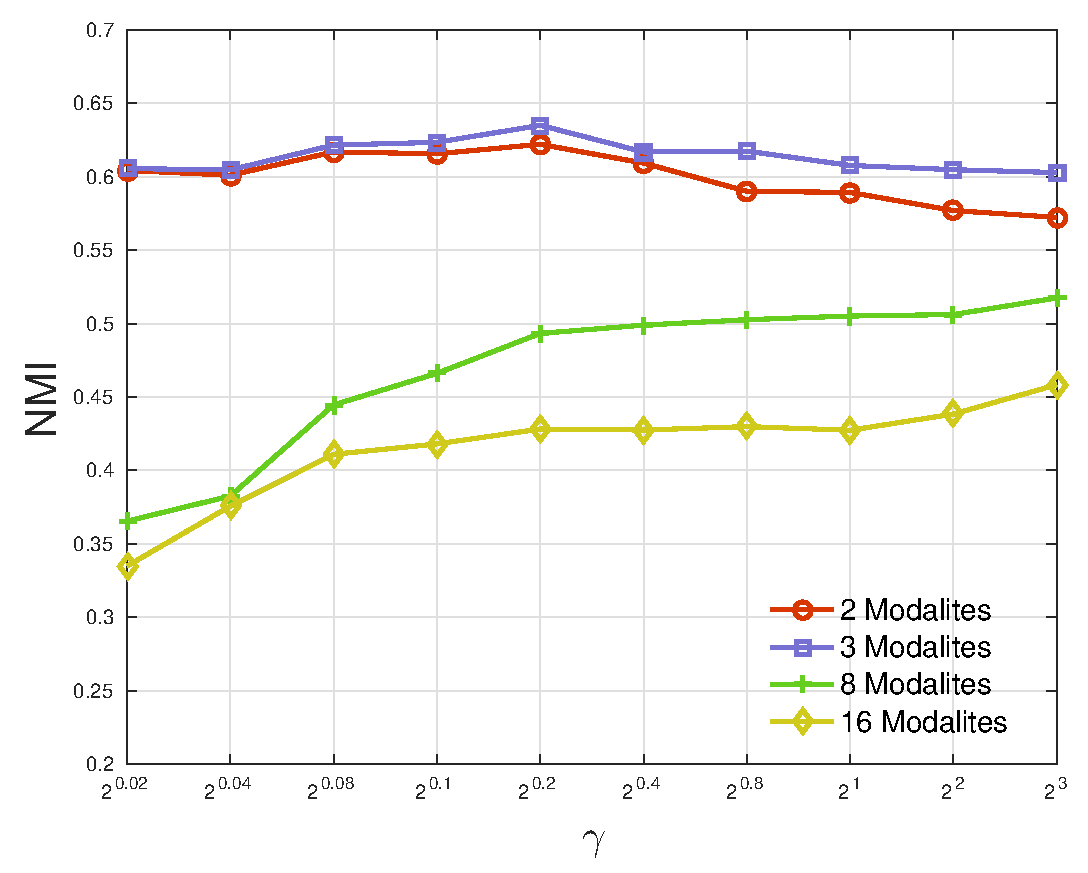
\includegraphics[width=0.495\textwidth]{chap3/corel_RWC_nmi.eps}
                    \label{fig3:rwc_corel}}
	\bisubcaptionbox{PASCAL VOC'07数据集}%
					{PASCAL VOC'07 dataset}
					[0.495\textwidth]{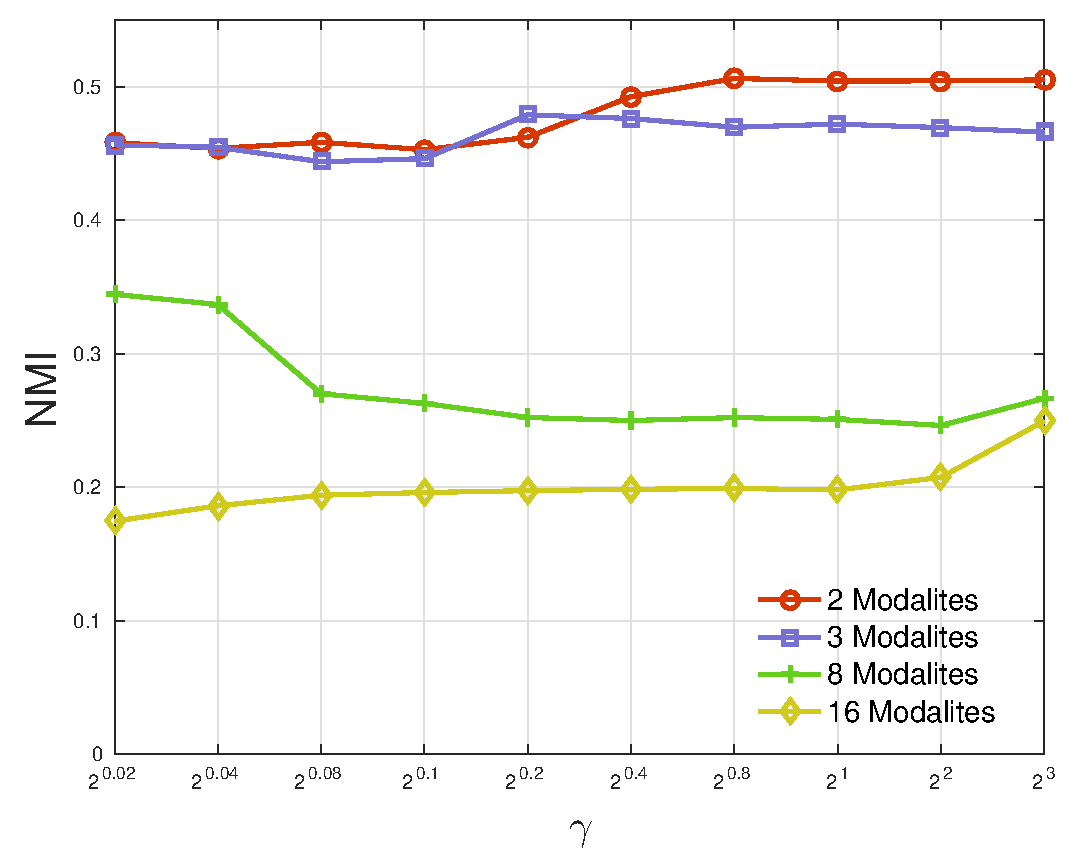
\includegraphics[width=0.495\textwidth]{chap3/voc_RWC_nmi.eps}
                    \label{fig3:rwc_voc}}
	\bicaption{在Corel 5k数据集和PASCAL VOC'07数据集上,超参数$\gamma$在不同的模态数量下对约束聚类效果的影响}{The influence of $ \gamma $ on Corel 5k and PASCAL VOC'07 datasets with different number of  modalities}
	\label{fig3:rwc}
\end{figure}

RWC方法在多模态聚类和多模态标签传播问题中较为普遍\cite{wang2009unified,xu2016discriminatively,xu2014multi}。 在通用的标签传播框架内,RWC方法可以被描述为以下优化问题:
\begin{equation}
\begin{split}
\mathop{\mathrm{min}}_{{f},{\alpha}}\;g({f},{\alpha})=&\frac{1}{2}\eta\; \|{f}-{y}\|^2_2+\frac{1}{2}{f}^T \sum_s(\alpha_s)^\gamma{\bar{{L}}}_s{f}, \\
s.t. \quad&\sum_s \alpha_s = 1;\\
&\;\alpha_s \ge 0,
\end{split}
\label{eq3:labelpro}
\end{equation}
此处,向量$ {y} \in  \mathbb{R}^{n} $为观测到的类标签信息,向量$ {\alpha} \in  \mathbb{R}^m$为可学习的模态权重($m$为不同的模态数量),$ {f} \in  \mathbb{R}^{n}$为标签传播的估计结果,$ \gamma > 1$ 和$ \eta $ 是手动设定的参数。拉普拉斯矩阵$ \bar{{L}}_s $ 由公式(\ref{eq3:jointW})中的 $ \bar{{W}}_s $  及其相应的对角权重矩阵 $ \bar{{D}}_s $生成。在固定$f$的情况下,可以忽略公式(\ref{eq3:labelpro})中的第一项,并通过拉格朗日函数求解$ {\alpha} $:
\begin{equation}
L({\alpha})=\sum_s(\alpha_s)^\gamma{f}^T {\bar{{L}}}_s{f} - \lambda ( \sum_s \alpha_s - 1)-\sum_s \mu_s \alpha_s,
\label{eq3:labelpro_L}
\end{equation}
其中$\lambda$和$\mu_s$为拉格朗日乘子,并且有$ \mu_s \ge 0$,$ \mu_s\alpha_s=0$。令函数(\ref{eq3:labelpro_L})对$ \alpha_s $的导数为零,能够得到
\begin{equation}
\gamma \alpha_s^{\gamma-1}{f}^T {\bar{{L}}}_s{f} =\lambda + \mu_s.
\label{eq3:labelpro_L_der}
\end{equation}
需要注意的是,为满足$ \mu_s\alpha_s=0 $,对于全部的$s$需要有$\mu_s=0 $。下文中将给出简要证明。

\begin{proposition}
   \label{thm3} 
    公式(\ref{eq3:labelpro_L_der})中,$\forall s \in \{1,\dots,m\}, \; \mu_s=0$。
\end{proposition}

\begin{proof}
    根据公式(\ref{eq3:labelpro_L})的约束条件已知$ \forall s \in \{1,\dots,m\}, \;\mu_s \ge 0$成立。

    现假设$\exists s \in \{1,\dots,m\}, \; \mu_s>0 $。由$ \mu_s\alpha_s=0 $可知必有$\alpha_s=0 $成立。
    则根据公式(\ref{eq3:labelpro_L_der})可知$\lambda + \mu_s = 0 $成立且$ \lambda<0 $成立。
    由于拉普拉斯矩阵$ {\bar{{L}}}_s $恒为半正定矩阵\cite{chung1997spectral},可知公式(\ref{eq3:labelpro_L_der})中$\forall s \in \{1,\dots,m\}, \;{f}^T {\bar{{L}}}_s{f} \ge 0$,即有$\forall s \in \{1,\dots,m\}, \; \lambda + \mu_s \ge 0 $。故:
    \begin{equation}
        \begin{split}
        \exists s \in \{1,\dots,m\}, \; \mu_s>0\; &\Rightarrow \;\lambda<0 \\&\Rightarrow \;\forall s \in \{1,\dots,m\}, \; \mu_s>0 \\&\Rightarrow \; \forall s \in \{1,\dots,m\}, \;\alpha_s=0.     
        \end{split}
    \end{equation}

    根据公式(\ref{eq3:labelpro_L})的约束条件$ \forall s \in \{1,\dots,m\}, \;\sum_s \alpha_s = 1$可知$ \exists s \in \{1,\dots,m\}, \;\alpha_s>0$,与假设产生矛盾,所以可知假设不成立,即有$\forall s \in \{1,\dots,m\}, \; \mu_s=0 $。
\end{proof}

将公式(\ref{eq3:labelpro_L_der})代入约束条件 $ \sum_s \alpha_s=1 $ 可以得到
\begin{equation}
\alpha_s = \frac{({f}^T \bar{{L}}_s{f})^\frac{1}{1-\gamma}}{\sum_s({f}^T \bar{{L}}_s{f})^\frac{1}{1-\gamma}}.
\end{equation}

不同于线性组合权重$ \alpha_s$, 模态的权重系数被松弛为指数形式 $ \alpha_s^\gamma $ 以避免求得平凡解使得 $ {\alpha} $中仅有一个元素为 $ 1 $ 其他元素全部为 $ 0 $。

值得一提的是,在约束传播中,存在两个待优化函数。最理想化的方法是将公式(\ref{eq3:sol-v})中的$ {F}_v $看作是权重系数$\alpha$的一个函数,并用这个函数替换优化问题(\ref{eq3:MMCP-h})中的约束矩阵$Y$,以求解权重系数$\alpha$的最优解。在将计算代价纳入考虑范围后,本章通过优化问题(\ref{eq3:baselinev})和(\ref{eq3:baselineh})来近似原优化问题的最小化子(minimizer)。在其中我们不通过$F_v$和$F_h$来区分竖直传播和水平传播的结果,统一采用$F$表示传播结果,仅使用目标函数$g_v({F})$和$g_h({F})$来区分竖直传播和水平传播过程。

\begin{equation}
\mathop{\mathrm{min}}_{{F}}\;g_v({F})=\frac{1}{2}\eta\;\mathrm{tr}(({F}-{Y})^T\bar{{D}}({F}-{Y}))+\frac{1}{2}\mathrm{tr}({F}^T \sum_s(\alpha_s^{old})^\gamma\bar{{L}}_s{F}).
\label{eq3:baselinev}
\end{equation}

\begin{equation}
\begin{split}
\mathop{\mathrm{min}}_{{F},{\alpha}}\;g_h({F},{\alpha})&=\frac{1}{2}\eta\;\mathrm{tr}(({F}-{Y})\bar{{D}}({F}-{Y})^T)+\frac{1}{2}\mathrm{tr}({F} \sum_s(\alpha_s)^\gamma\bar{{L}}_s{F}^T), \\
s.t.\quad\;& \sum_s \alpha_s = 1;\\ & \; \alpha_s \ge 0.
\end{split}
\label{eq3:baselineh}
\end{equation}

假设公式(\ref{eq3:baselinev})中的权重系数为固定的常数向量,用$ {\alpha}^{old} $表示,而只通过优化问题(\ref{eq3:baselineh})更新权重系数,即$\alpha$。通过将向量$\alpha$的值赋给$ {\alpha}^{old} $,可以迭代求解权重系数和约束传播结果$F$。

在固定$\alpha$的情况下,先求解公式(\ref{eq3:baselinev})并将其最优解作为$Y$代入公式(\ref{eq3:baselineh}),可求得$F$为
\begin{equation}
{F} = \eta^2(\eta\bar{{D}}+\bar{{L}})^{-1}\bar{{D}} {Y}\bar{{D}}(\eta\bar{{D}}+\bar{{L}})^{-1}, 
\label{eq3:bl_F}
\end{equation}
其中$\bar{{D}} = \sum_s (\alpha_s^{old})^\gamma  \bar{{D}}_s $ 且 $  \bar{{L}} = \sum_s (\alpha_s^{old})^\gamma  \bar{{L}}_s $,这与公式( \ref{eq3:unifiedW})相似。

在固定$F$的情况下,由公式(\ref{eq3:baselineh})可求得向量$\alpha$中元素为
\begin{equation}
\alpha_s = \frac{\mathrm{tr}({F} \bar{{L}}_s{F}^T)^\frac{1}{1-\gamma}}{\sum_s \mathrm{tr}({F} \bar{{L}}_s{F}^T)^\frac{1}{1-\gamma}}, 
\end{equation}
并且更新${\alpha}^{old}$:$ {\alpha}^{old} \leftarrow {\alpha}$。由于根据公式(\ref{eq3:bl_F})计算出的$F$为对称矩阵,因此从竖直传播或水平传播中学习权重系数在结果上是等价的。

从公式(\ref{eq3:baselinev})和公式(\ref{eq3:baselineh})中,可以观察到超参数$ \gamma $在RWC方法中起到核心作用。每个模态的权重系数受$ \gamma $控制。 特别地,当$ \gamma \rightarrow \infty$时,该算法将生成全部相等的权重。而当 $ \gamma $趋近于 $ 1 $时,该算法将只选择一个具有最优一致性的模态,即令$  \mathrm{tr}({F} \bar{{L}}_s{F}^T) $最小的模态。我们在Corel 5k数据集和PASCAL VOC' 07数据集上,评估了超参数$\gamma$对在不同的模态数量下对约束聚类效果的影响。图\ref{fig3:rwc}展示了RWC方法在不同的$\gamma$取值情况下的约束聚类性能评估结果,评估测度为归一化互信息(normalized mutual information, NMI)。我们可以观察到,当有极多模态数量的情况下,例如16个模态,RWC方法很难针对每个模态生成合适的权重。因而,当有16个模态时,RWC方法在$ \gamma = 2^3 $处取得最佳性能,此时各个模态的权重几乎相等。此外,图\ref{fig3:rwc}还显示$\gamma$的最佳选择在不同的数据集和不同数量的模态的情况下有所不同,很难选择可以广泛使用的$\gamma$值。在第\ref{sec3:exp}节的实验结果评估中,我们将选择在图\ref{fig3:rwc}中给出最优表现的$ \gamma $值,这一点与许多先前文献中的工作一样。然而,在实际的半监督问题中,这样的超参数选择策略往往是不可行的,因为经常没有足够标注数据可以作为验证集进行参数选择。

图\ref{fig3:cvg}给出了RWC方法的收敛曲线。可以看出优化问题的近似,公式(\ref{eq3:baselinev})和公式(\ref{eq3:baselineh}),能够在两到三次迭代后相对收敛。在第\ref{sec3:opt}节将给出更多的收敛性讨论。

\begin{figure}[t]
	\centering
	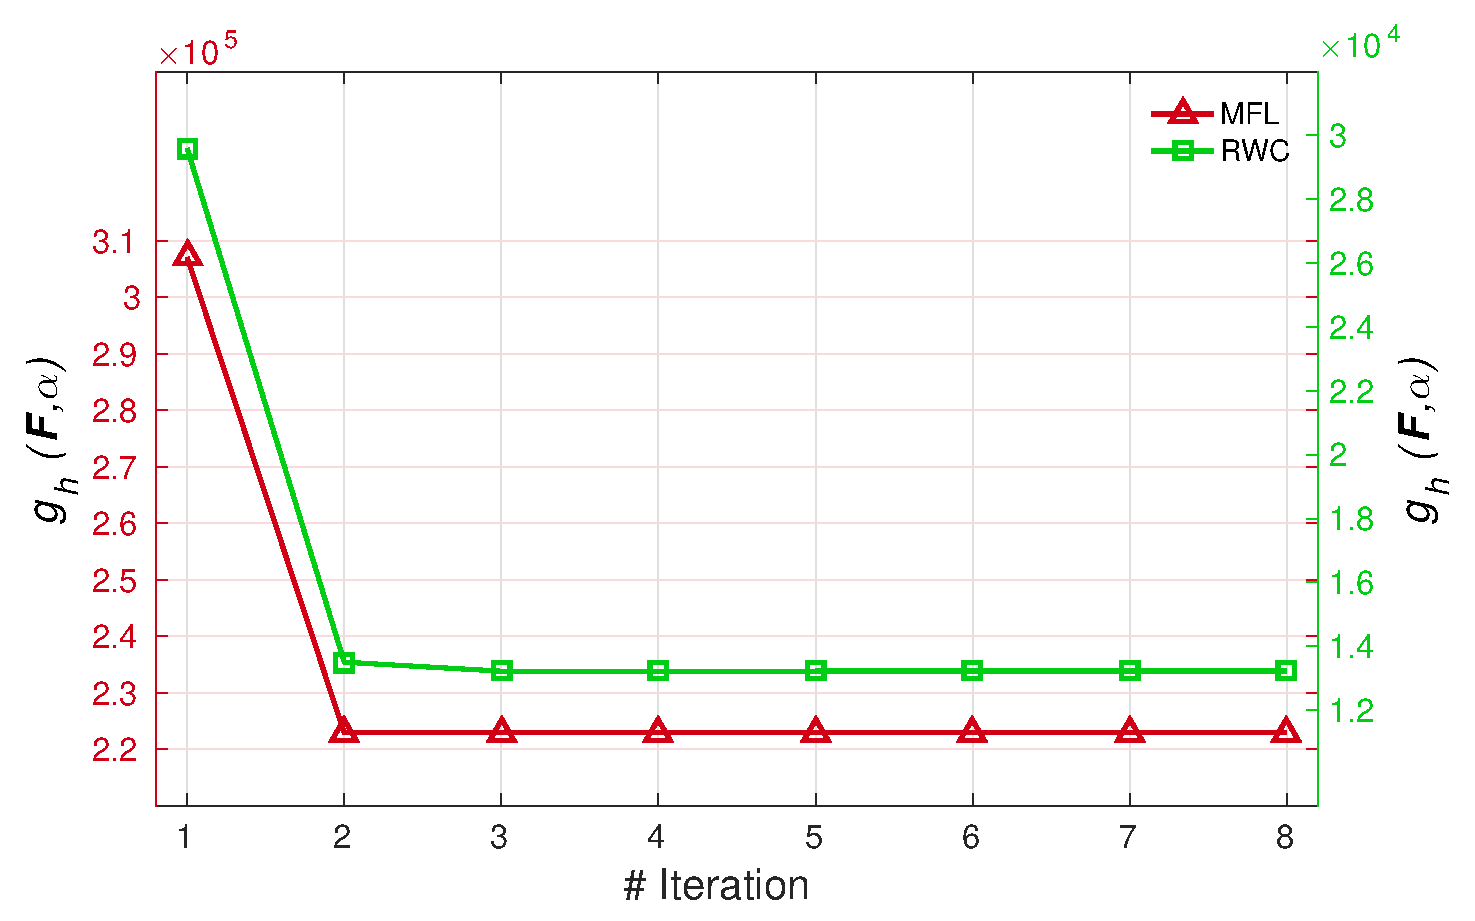
\includegraphics[width = 0.9\columnwidth]{chap3/cvg.eps}
	\bicaption{所提出的RWC方法和MFL方法在Corel 5k数据集上的收敛曲线}{The convergence curve of the proposed RWC and MFL on Corel 5k dataset}
	\label{fig3:cvg}
\end{figure}

\subsection{多模态融合学习的公式化}
本章所提出的多模态融合学习(Multi-modal Fusion Learning,MFL)方法基于以下假设:在使用完美的权重系数的情况下,可以从每种模态的相似性矩阵中以最小的损失重建出观察到的约束。 换句话说,我们可以将数据中的成对约束视为每个模态的相似性的凸组合。而在观察到一部分成对约束的情况下,即已知约束矩阵$Y$,可以通过回归的方式来重构其他未观察到的约束。

基于这样的假设,我们将重构误差引入多模态约束传播的框架中。
假设在矩阵$Y$中有$l$个观测到的成对约束,即$Y$中有$l$个非零元素。然后可以对这$l$个不同的约束进行编号。定义两个函数$ r(i) $ 和 $ c(i) $,其中$ r(i) $ 的函数值为编号为$i$的约束在矩阵$Y$中的行号,函数$ c(i) $的值为相应的列号($i \in \{1,\dots,l\}$)。
则可以通过元素$ y_{r(i),c(i)} $对$Y$中的第$i$个约束进行定位和检索。基于这两个函数,可以构建约束向量$ {z} \in \mathbb{R}^n$:
\begin{equation}
z_i = \begin{cases}1,\quad\quad &\text{if}\;\; y_{r(i),c(i)} =1; \\
0, \quad\quad &\text{otherwise}.
\end{cases}
\end{equation} 
此处可理解为,must-link在向量$z$中对应$1$,cannot-link对应$0$,未观测到的约束不出现在约束向量$z$中。

同时可以根据所有模态的相似性矩阵$ \{{W}_s|s\in\{1,\dots,m\}\} $构建相应的基矩阵$ {S} \in \mathbb{R}^{l\times m}$($l$为约束的数量,$m$为模态数量),
\begin{equation}
 {S}_{i,s} = w_{r(i), c(i), s}.
\end{equation}
则重构误差可以定义为
\begin{equation}
error = \|{S}{\alpha}-{z}\|_2^2,
\end{equation}
这里 $ {\alpha} $ 为权重系数。
由于${W}_s$为稀疏的相似性矩阵,所以该重构误差可以理解为,对于相似性为$0$的成对关系应对应于向量$z$中的cannot-link值即$0$,而相似性大于$0$的成对关系对应于向量$z$中的must-link值即$1$。

需要引起注意的是,$z$中的must-link和cannot-link的比例大约为$1:c-1 $,其中$c$为类别数。如果从高度稀疏的相似性矩阵中生成矩阵 $S$,则在矩阵 $S$中会存在极大量的零元素,这将使得样本分布不均衡,重构变得很困难。所以与用于构造拉普拉斯矩阵$ \bar{{L}}_s $的高度稀疏的相似性矩阵不同,基矩阵$S$ 由近邻数为$ k=\frac{\#sample}{\#cluster} = \frac{n}{c}$ 的相对密集的相似性矩阵生成。在这种情况下 矩阵$S$中零元素与非零元素的比例 和 向量$z$中两者比例大致相似。

将重构误差纳入考虑范围后,可以设计出一个优化问题以同时最小化传播误差和重构误差。与RWC方法中的近似方式相似,我们仅从水平方向的约束传播学习权重系数,从而可以得出以下优化问题:

\begin{equation}
\mathop{\mathrm{min}}_{{F}}\;g_v({F})=\frac{1}{2}\eta \;\mathrm{tr}(({F}-{Y})^T\bar{{D}}({F}-{Y}))+\frac{1}{2}\mathrm{tr}({F}^T \sum_s\alpha_s^{old}\bar{{L}}_s{F}),
\label{eq3:MFL_v}
\end{equation}
及
\begin{equation}
\begin{split}
\mathop{\mathrm{min}}_{{F},{\alpha}}\;g_h({F}, {\alpha})=&\frac{1}{2}\eta\;\mathrm{tr}(({F}-{Y})\bar{{D}}({F}-{Y})^T)+\frac{1}{2}\mathrm{tr}({F} \sum_s\alpha_s\bar{{L}}_s{F}^T) \\ &+\frac{1}{2}\zeta\|{S}{\alpha} - {z}\|_2^2,\\
s.t. \quad\;& \sum_s \alpha_s = 1;\\ &\; \alpha_s \ge 0.
\end{split}
\label{eq3:MFL}
\end{equation}

在公式(\ref{eq3:MFL})中,我们采用了与E$^2$CP\cite{lu2010constrained} 和MMCP\cite{fu2011multi}方法中相同的$ \eta $取值,即$ \eta = 0.25 $,并且将竖直方向的传播问题(\ref{eq3:MFL_v})的最优解作为水平方向传播约束矩阵 $ {Y} $。至于参数 $ \zeta $,我们认为在重构误差中的元素应该与$ \mathrm{tr}({F} \sum_s\alpha_s\bar{{L}}_s{F}^T) $中的元素具有相似的重要性。 如果将$ \sum_s\alpha_s\bar{{L}}_s $ 看作一个距离度量矩阵,则$ \mathrm{tr}({F} \sum_s\alpha_s\bar{{L}}_s{F}^T) $ 可以认为时投影后的$ {F}^T $的Frobenius 范数的平方,即是$\#sample^2=n^2$个元素的平方和。同时,重构误差也可以被看作是一个Frobenius范数平方的特例,其中包含了$ \#constraint = l $ 个元素。所以选择 $ \zeta = \frac{\#sample^2}{\#constraint}=\frac{n^2}{l} $使这两项处于同一重要性级别。

公式(\ref{eq3:MFL})可以利用观察到的成对约束来学习权重系数,而不是仅仅从与约束传播相同的优化目标函数中学习一个比率。使用更多的观察到的信息将能够提高所提出的方法的鲁棒性。通过组合重构误差和约束传播误差,多模态约束传播的目标函数不再是单模态约束传播目标函数的简单组合,并且不会出现第\ref{sec3:rwc}节中提到的平凡解,因此也不需要采用指数形式对权重系数进行松弛。

\subsection{多模态融合学习的优化}
\label{sec3:opt}

\begin{algorithm}[t]
	\SetKwInput{KwData}{输入}
    \SetKwInput{KwResult}{输出}
	\caption{多模态融合学习}
	\label{alg3:MFL}
	\KwData{相似性矩阵 $W_s$;约束矩阵$Y$;基矩阵 $S$;聚类数量$c$。}
    \KwResult{统一的相似性矩阵 $W^*$。}
    选择初始化的可行权重参数向量$ {\alpha}^0_0 $,$ i = 0 $;\\
    \Repeat{收敛}{
        根据公式(\ref{eq3:MFL_F})计算$ {F}_{i+1} $。\\
        选择初始化的乘子$ \lambda_0 $ 和惩罚参数$ \mu_0 $; 初始化$ \varepsilon_0 > 0 $; $ j = 0 $;\\
        \Repeat{收敛}{
            通过投影梯度法近似求解公式(\ref{eq3:MFL_L})${\alpha}^i_j =  \mathrm{arg}\mathop{\mathrm{min}}\limits_{{\alpha}}\;\mathcal{L}({\alpha},\lambda_j;\mu_j)$;\\                        
            \uIf{$ \|\mathbf{1}^T{\alpha}_j^i- 1\| \le \varepsilon_j $}{
                $ \lambda_{j+1} \leftarrow \lambda_j - \mu_j(\mathbf{1}^T{\alpha}_j^i- 1) $;\\
                $ \mu_{j+1} \leftarrow \mu_j $;\\
                $ \varepsilon_{j+1} \leftarrow \varepsilon_j \mu^{-0.9 }$;\\
            }
            \Else{
                $ \lambda_{j+1} \leftarrow \lambda_j$;\\
                $ \mu_{j+1} \leftarrow 100\mu_j $;\\
                $ \varepsilon_{j+1} \leftarrow \mu^{-0.1 }$;\\
            }

            $ j\leftarrow j+1 $;\\
        }
        $ i\leftarrow i+1 $;\\
    }
    根据公式(\ref{eq3:rSa}),通过整流Sigmoid激活函数,由$F_i$生成$W^*$。
\end{algorithm}

MFL方法的求解可以分解为两个子问题,并能够通过交替迭代法求解。在本节中,我们将描述优化求解过程的一些细节。

    \textbf{固定$\alpha$求解$F$}:

当权重系数$\alpha$固定时,公式(\ref{eq3:MFL})可以被化简为公式(\ref{eq3:MMCP-h})。因此,我们可以发现$F$的解与公式(\ref{eq3:bl_F})非常相似:
\begin{equation}
{F} = \eta^2(\eta\bar{{D}}+\bar{{L}})^{-1}\bar{{D}} {Y}\bar{{D}}(\eta\bar{{D}}+\bar{{L}})^{-1},
\label{eq3:MFL_F}
\end{equation}
在其中$  \bar{{D}} = \sum_s \alpha_s  \bar{{D}}_s $ and $  \bar{{L}} = \sum_s \alpha_s \bar{{L}}_s $。

    \textbf{固定$F$求解$\alpha$}:

当$F$固定时,公式(\ref{eq3:MFL})可以被变形为有界约束的二次优化问题(bound-constrained quadratic optimization problem):
\begin{equation}
\begin{split}
\mathop{\mathrm{min}}_{{\alpha}}\;&\frac{1}{2}\mathrm{tr}({F} \sum_s\alpha_s\bar{{L}}_s{F}^T)+\frac{1}{2}\zeta\|{S}{\alpha} - {z}  \|_2^2,\\
s.t.\quad& \sum_s \alpha_s = 1;\\ &\; \alpha_s \ge 0.
\end{split}
\label{eq3:MFL_ALM}
\end{equation}    
考虑到公式(\ref{eq3:MFL_ALM})的计算复杂度与$\alpha$的维度相关,即与模态数量相关,并且$\alpha$为低维向量,我们采用了增广拉格朗日方法\cite{bertsekas1982constrained}优化所提出的目标函数。
我们沿用了文献\parencite{nocedal2006numerical} 和文献\parencite{bertsekas1982constrained}中所介绍的有界约束拉格朗日优化方法(bound-constrained Lagrangian,BCL)的详细策略。通过将公式(\ref{eq3:MFL_ALM})中的等式约束纳入增广拉格朗日方法可以生成子问题
\begin{equation}
\begin{split}
\mathop{\mathrm{min}}_{{\alpha}}\;\mathcal{L}({\alpha},\lambda;\mu) =&\frac{1}{2}\zeta\|{S}{\alpha} - {z}\|_2^2+\frac{1}{2}\sum_s\alpha_s\mathrm{tr}({F} \bar{{L}}_s{F}^T) \\
&- \lambda(\mathbf{1}^T{\alpha}-1)+\frac{\mu}{2}(\mathbf{1}^T{\alpha}-1)^2\\
s.t.\quad &\alpha_s \ge 0.
\end{split}
\label{eq3:MFL_L}
\end{equation}
我们采用了投影梯度法(gradient projection method)对公式(\ref{eq3:MFL_L})中的子问题进行近似求解,然后更新乘子$ \lambda $ 和惩罚系数 $ \mu $,并重复迭代该过程\cite{nocedal2006numerical,conn1992lancelot}。算法\ref{alg3:MFL}对所提出的方法、其中的增广拉格朗日方法迭代求解步骤以及后处理进行了总结。

图\ref{fig3:cvg}展示了MFL方法的收敛曲线。可以发现,一旦在RWC方法和MFL方法中将权重系数分解为$ {\alpha}^{old} $ 和 $ {\alpha} $两部分,$ {\alpha}^{old} $可以被看作为常数向量。然后,我们学习MMCP算法的做法,将水平方向约束传播目标函数(公式(\ref{eq3:baselineh})和公式(\ref{eq3:MFL}))中的约束矩阵$Y$代换为竖直方向约束传播所求得的最优解。通过代换,仅需要考虑更新传播结果$F$和系数$\alpha$。下文将简要论述该迭代算法的收敛性。

由于对角权重矩阵$ \bar{{D}}_s $和拉普拉斯矩阵$\bar{L}_s$都为半正定矩阵,其凸组合$ \sum_s\alpha_s\bar{{L}}_s $也为半正定矩阵。因此,公式(\ref{eq3:MFL})的目标函数中三项皆为非负值,且有$ g_h({F}, {\alpha}) \ge 0 $。我们可以通过任意可行解$F_0$对$F$的解集进行定界,以得到一个$(F, \alpha)$的紧致解集。例如,在原优化问题基础上增加一个辅助约束:
\begin{equation}
        \frac{1}{2}\eta\;\mathrm{tr}(({F}-{Y})\bar{{D}}({F}-{Y})^T)  \le g_h({F}_0, {\alpha}),
\end{equation}
并且优化问题(\ref{eq3:MFL})的最优解恒满足此辅助约束条件。极值定理(extreme value theorem)保证了从非空紧空间到一个实数子集的连续映射函数$ g_h({F}, {\alpha})$必然存在最优解$({F}^*, {\alpha}^*) $使得函数取得最小值。

更进一步地,原目标函数为分别关于$F$和$\alpha$的凸函数。对于一个迭代序列集合$ \{({F}^{(t)}, {\alpha}^{(t)})\} $,有
\begin{equation}
    g_h({F}^{(t)}, {\alpha}^{(t)}) \ge \mathop{\mathrm{min}}_{{F}} g_h({F}, {\alpha}^{(t)}) = g_h({F}^{(t+1)}, {\alpha}^{(t)}) \ge \mathop{\mathrm{min}}_ {{\alpha}} g_h({F}^{(t+1)}, {\alpha}) =g_h({F}^{(t+1)}, {\alpha}^{(t+1)}).
\end{equation}
所以,针对$F$和针对$\alpha$的迭代步骤都可以最小化目标函数(\ref{eq3:MFL}),这显示了所提出的RWC和MFL算法都可以有效收敛。如图\ref{fig3:cvg}所示,MFL算法可以在大约两轮迭代中近似收敛。

\subsection{后处理流程}
在先前关于约束传播的大多数工作中,传播结果$F$被用于完善原始$k$-NN相似性矩阵$W$:
\begin{equation}
w^*_{ij} = 
\begin{cases}
1-(1-f_{ij})(1-w_{ij}), \qquad &f_{ij}\ge 0;\\
(1+f_{ij})w_{ij}, &f_{ij}< 0,
\end{cases}
\label{eq3:refine}
\end{equation}
其中,$ w_{ij} $ 为数据实例 $ x_i $ 和$ x_j $之间的$k$-NN相似性。

上述通过调整获得最终解的方法有两个不足之处。一方面,传播结果$ {F} $的信息未被充分利用。另一方面,求得的最终结果高度取决于原始相似性矩阵的质量。在我们的RWC和MFL方法中,我们放弃了原始的相似性矩阵,而采用整流Sigmoid激活函数从$F$中直接生成统一的相似性矩阵:
\begin{equation}
w^*_{ij} = 
\begin{cases}
\frac{1}{1+\text{exp}(-f_{ij}/\sigma)}, \qquad &\text{if }f_{ij}>0;\\
0, &\text{otherwise, }
\end{cases}
\label{eq3:rSa}
\end{equation}
在这里,$ \sigma  $为矩阵$F$中所有元素的强度的均值。整流Sigmoid函数使得统一的相似性矩阵完全依赖于传播的结果。此外,使用整流Sigmoid函数比完善方法更具有可解释性。对于传播结果$F$中的正元素,Sigmoid函数部分将传播结果的数值投影到$0.5$到$1$之间,这可以被解释为一个联合概率。对于负元素,负值表示两个数据样本被预测为不属于同一个类别。因此,我们根据$k$-NN热力核的定义,在统一相似性矩阵中将这些约束设置为$0$,而不是通过Sigmoid函数得到一个正值的相似性。

随后,我们对$ W^* $应用谱聚类方法\cite{von2007tutorial}进行特征投影,并通过$ k$-means聚类对结果进行评估。

\subsection{权重系数的稀疏性}
\label{sec3:dis}
如果基矩阵$S$的列向量线性无关,我们可以将矩阵$S$的左逆矩阵表示为$ {S} ^+ = ({S}^T{S})^{-1}{S}^T$。定义向量 $ {h} \in  \mathbb{R}^{m} $为
\begin{equation}
h_s = \text{tr}({F} \bar{{L}}_s{F}^T).
\end{equation}
我们可以将优化问题(\ref{eq3:MFL_ALM})变形为
\begin{equation}
\begin{split}
\mathop{\mathrm{min}}_{{\alpha}}\;&\|{S}{\alpha} - ( {z} - \frac{1}{2\zeta}{S}^+ {h}) \|_2^2,\\
s.t.\quad& \sum_s \alpha_s = 1;\\ &\; \alpha_s \ge 0.
\label{eq3:nnls}
\end{split}
\end{equation}

公式(\ref{eq3:nnls})是一个在凸约束$ \sum_s \alpha_s = 1 $下的非负最小二乘法(non-negative least square,NNLS)问题的特例。在我们所提出的MFL中可以观察到一些NNLS问题的特性。
在回归系数上的非负约束具有与显式的稀疏正则化项相似的效果,并且NNLS有与LASSO \cite{tibshirani1996regression}相当的稀疏性能,这一点在文献\parencite{slawski2011sparse}和文献\parencite{slawski2013non}中都有进一步的论证,并且在我们的实验中也能够观察到这种性质。随着我们为所提出的算法提供更多的模态信息,权重系数的稀疏性变得更加明显。当我们在8种不同模态上应用所提出的方法时,我们注意到大约有2或3个模态的权重为零。当我们使用的模态数达到16个时,将有大约一半的零权重。因此,MFL可以用作模态选择器,并且仅在候选列表中保留有帮助的模态。这也是当存在极多不同模态时我们的方法具有鲁棒表现的主要原因。

\begin{table}[tb]
	\bicaption{在Corel 5k和PASCAL VOC'07数据集上采用2种模态情况下的聚类性能}{Clustering performance of 2 modalities on Corel 5k and PASCAL VOC'07}
	\label{tab3:2modal}
	\centering
	\setlength{\tabcolsep}{15pt}
	\begin{tabular}{lcccc}
		\toprule
		&\multicolumn{2}{c}{Corel 5k} & \multicolumn{2}{c}{PASCAL VOC'07} \\
		\cmidrule(lr){2-3}
		\cmidrule(lr){4-5}
		& ACC\% & NMI\% & ACC\% & NMI\% \\
		\midrule
		NCuts\cite{shi2000normalized} & 40.23 & 50.68 & 34.11 & 36.06 \\ 
		E$^2$CP\cite{lu2010constrained} & 49.76 & 59.05 & 46.84 & 45.26 \\
		MCMCP\cite{fu2012modalities} & 50.20 & 60.42 & 46.00 & 44.13 \\  
		MMCP\cite{fu2011multi} & 43.22 & 53.10 & 51.42 & 46.99 \\ 
		UCP\cite{lu2013unified} & 48.98 & 59.39 & 36.43 & 24.31 \\ 
		MSCP\cite{lu2013exhaustive} & 50.18 & 60.74 & 37.33 & 32.82 \\ 
		\midrule
		SW & 48.44 & 56.33 & \textbf{57.44} & \textbf{50.28} \\ 
		RWC & \textbf{54.97} & 62.11 & 56.80 & 50.24 \\ 
		MFL & 54.87 & \textbf{62.32} & 55.07 & 48.55 \\ 
		\bottomrule
	\end{tabular}
\end{table}


\section{实验结果}
\label{sec3:exp}
在本节中,我们报告一些实验结果以证明所提出的MFL方法和基线方法RWC的有效性。我们在两个公开可用的数据集上进行了大量的约束聚类实验,展示了所提出的方法在不同的模态数量下的聚类性能及其模态选择能力。
\subsection{数据集描述}
在我们的实验中,我们采用了INRIA\footnote{\url{http://lear.inrialpes.fr/people/guillaumin/data.php}}发布的两个被广泛使用的多模态特征数据集\cite{guillaumin2009tagprop}:
\begin{itemize}
    \item {\textbf{Corel 5k}}。Corel 5k自然图像数据集是一个重要的基准数据集,在许多不同任务上被广泛采用。Corel 5k具有50个类别和4,999张自然图像。数据集中的每张图像都有一组关键字描述,这些关键词选取自一个包含260个单词的关键词词典。
    \item {\textbf{PASCAL VOC'07}}。PASCAL VOC'07数据集\cite{pascal-voc-2007}包含20个图像类别和9,963张图像。据集中的所有图像均带有一个或多个类别标注。文字描述基于一个包含804个关键词的词典。
\end{itemize}

INRIA特征数据集\cite{guillaumin2009tagprop}对Corel 5k和PASCAL VOC'07数据集中的图像进行了相同标准的特征抽取,分别生成了一个多模态特征数据集。对于每一个数据集,INRIA特征中包含了16种不同的特征,其中包含了15种视觉特征(1种Gist特征,6种颜色直方图特征和8种词袋特征):\textit{DenseSift,DenseSiftV3H1,HarrisSift,HarrisSiftV3H1,DenseHue,DenseHueV3H1,HarrisHue,HarrisHueV3H1,Rgb,RgbV3H1,Lab,LabV3H1,Hsv,HsvV3H1,Gist}。以及1种关键词表述特征:\textit{tag}。
此外,为多模态半监督学习任务而创建的这些特征数据集也可以被视为多模态多视图数据集,在我们的实验中,我们将每种特征视为一个独立的模态。

\subsection{对照算法介绍}

\begin{table}[t]
	\bicaption{在Corel 5k数据集上采用3个、8个和16个模态的聚类性能}{Clustering performance of 3, 8 and 16 modalities on Corel 5k}
	\label{tab3:modal_corel}
	\centering
	\setlength{\tabcolsep}{8pt}
	\begin{tabular}{l*{6}{c}}
		\toprule
		&\multicolumn{2}{c}{3 modalities} & \multicolumn{2}{c}{8 modalities} & \multicolumn{2}{c}{16 modalities} \\
		\cmidrule(lr){2-3}
		\cmidrule(lr){4-5}
		\cmidrule(lr){6-7}
		& ACC\% & NMI\% & ACC\% & NMI\% & ACC\% & NMI\% \\
		\midrule
		NCuts\cite{shi2000normalized} & 44.98 & 54.33 & 38.61 & 49.27 & 32.07 & 42.11 \\ 
		E$^2$CP\cite{lu2010constrained} & 52.64 & 61.14 & 40.19 & 50.17 & 28.80 & 39.17 \\ 
		MCMCP\cite{fu2012modalities} & 49.15 & 59.90 & 36.72 & 51.56 & 36.24 & 51.12 \\ 
		MMCP\cite{fu2011multi} & 48.50 & 56.58 & 37.82 & 48.33 & 32.98 & 43.63 \\ 
		\midrule
		SW & 51.83 & 60.40 & 42.61 & 50.53 & 33.74 & 42.81 \\
		RWC & 55.51 & 63.44 & 43.60 & 51.60 & 36.56 & 45.43 \\
		MFL & \textbf{56.36} & \textbf{63.99} & \textbf{57.04} & \textbf{64.11} & \textbf{56.67} &\textbf{ 64.09} \\
		\bottomrule
	\end{tabular}
\end{table}

我们将所提出的MFL和RWC算法和一些在第\ref{sec3:intro}节中提及的目前先进的方法以及部分基线方法进行了比较。
以下是我们在实验中所用于对比的算法:
\begin{itemize}
    \item {\textbf{MMCP}}。正如在第\ref{sec3:intro}节中所提到的那样,由于在半监督聚类问题的设置中,很难手动确定每个模态的重要性。在我们的实验中,我们为MMCP\cite{fu2011multi}中的每个模态设置了同等的重要性。
    \item {\textbf{SW}}。SW(same weight)是本文提出的另一个基线方法,表示所有模态具有的权重相同。在SW中,我们删除了MFL中的权重学习步骤,并强制每个模态具有相同的权重。在我们的实验中,SW方法与MMCP算法相似。它们之间的唯一区别在于,SW采用了整流Sigmoid激活函数来生成最终的相似性矩阵,而MMCP采用了公式(\ref{eq3:refine})中调整完善的方法。
    \item {\textbf{MSCP}}。Multi-Source Constraint Propagation(MSCP)\cite{lu2013exhaustive}方法专注于两种模态上的约束传播。在本节中,我们将在两种模态的情况下将我们的方法与MSCP进行比较。
    \item {\textbf{UCP}}。Unified Constraint Propagation(UCP)\cite{lu2013unified}方法同时进行了视图内和视图间的约束传播,这种方法同样是针对两种模态的情况所设计的。
    \item {\textbf{MCMCP}}。Modalities Consensus for Multi-modal Constraint Propagation(MCMCP)\cite{fu2012modalities}方法通过迭代法求解约束传播问题。在每一行迭代中,MCMCP方法会在每一个模态上分别进行一次传播,这使得整个算法非常耗时。
    \item {\textbf{E$^2$CP}}。E$^2$CP\cite{lu2010constrained}方法是一个单模态约束传播方法,但我们依然将该方法引入我们的实验中作为一个基线方法。在我们的实验中,我们在每个模态上单独使用E$^2$CP,然后将算法在每个模态上生成的经传播调整完善后的相似性矩阵求平均,以此作为多模态的E$^2$CP方法结果。
    \item {\textbf{NCuts}}。在实验中,我们报告了没有传播过程而仅采用Normalized Cuts(NCuts)\cite{shi2000normalized}的聚类结果作为参考。在对NCuts算法进行实验时,我们用相同的权重对各模态的相似性矩阵取平均值。
\end{itemize}

\subsection{实验设置}

\begin{table}[t]
	\bicaption{在PASCAL VOC'07数据集上采用3个、8个和16个模态的聚类性能}{Clustering performance of 3, 8 and 16 modalities on PASCAL VOC'07}
	\label{tab3:modal_voc}
	\centering
	\setlength{\tabcolsep}{8pt}
	\begin{tabular}{lcccccc}
		\toprule
		&\multicolumn{2}{c}{3 modalities} & \multicolumn{2}{c}{8 modalities} & \multicolumn{2}{c}{16 modalities} \\
		\cmidrule(lr){2-3}
		\cmidrule(lr){4-5}
		\cmidrule(lr){6-7}
		& ACC \% & NMI \% & ACC \% & NMI \% & ACC\% & NMI\%		\\
		\midrule 
		NCuts\cite{shi2000normalized} & 26.76 & 25.04 & 23.07 & 21.26 & 22.31 & 18.40 \\
		E$^2$CP\cite{lu2010constrained} & 40.46 & 39.50 & 29.39 & 26.40 & 25.66 & 21.29 \\ 
		MCMCP\cite{fu2012modalities} & 34.85 & 27.34 & 29.36 & 24.79 & 29.80 & 24.98 \\  
		MMCP\cite{fu2011multi} & 38.29 & 36.14 & 29.04 & 26.40 & 27.85 & 24.90 \\
		SW & 49.96 & 45.77 & 31.67 & 24.25 & 29.98 & 20.15 \\ 
		RWC & 53.27 & 47.55 & 42.07 & 34.33 & 29.08 & 24.97 \\ 
		MFL & \textbf{56.66} & \textbf{49.98} & \textbf{54.95} & \textbf{49.06} & \textbf{56.35} & \textbf{49.86} \\ 
		\bottomrule
	\end{tabular}
\end{table}
为了评估这些方法的聚类性能,我们在实验中采用准确率(accuracy,ACC)和归一化互信息(normalized mutual information,NMI)作为聚类结果的性能测度。
由于约束传播方法的性能在某种程度上取决于约束矩阵${Y}$的选择。我们在每个实验中生成多个约束矩阵,并在本节中报告算法在不同约束矩阵上的平均性能。
我们在$k$-means阶段部署30次聚类,并选择类内和最小的聚类结果作为$k$-means阶段的结果。

实验中,除RWC中的$\gamma $之外,所有参数都有相同的参数选择标准。在RWC和MFL方法中传播参数$ \eta $如同MMCP和E$^2$CP一样都为$ 0.25 $。我们将$k$-NN近邻数量设置为$ k = \mathrm{Round}(\mathrm{log}_2(\frac{n}{c}))$,其中$ n $是数据实例的数量,$ c $是类别数。谱聚类中的特征嵌入维数为$ c + 1 $。


\begin{figure}[t]
	\centering
	\bisubcaptionbox{Corel 5k数据集上的ACC结果}%
					{ACC on  Corel 5k}
					[0.495\textwidth]{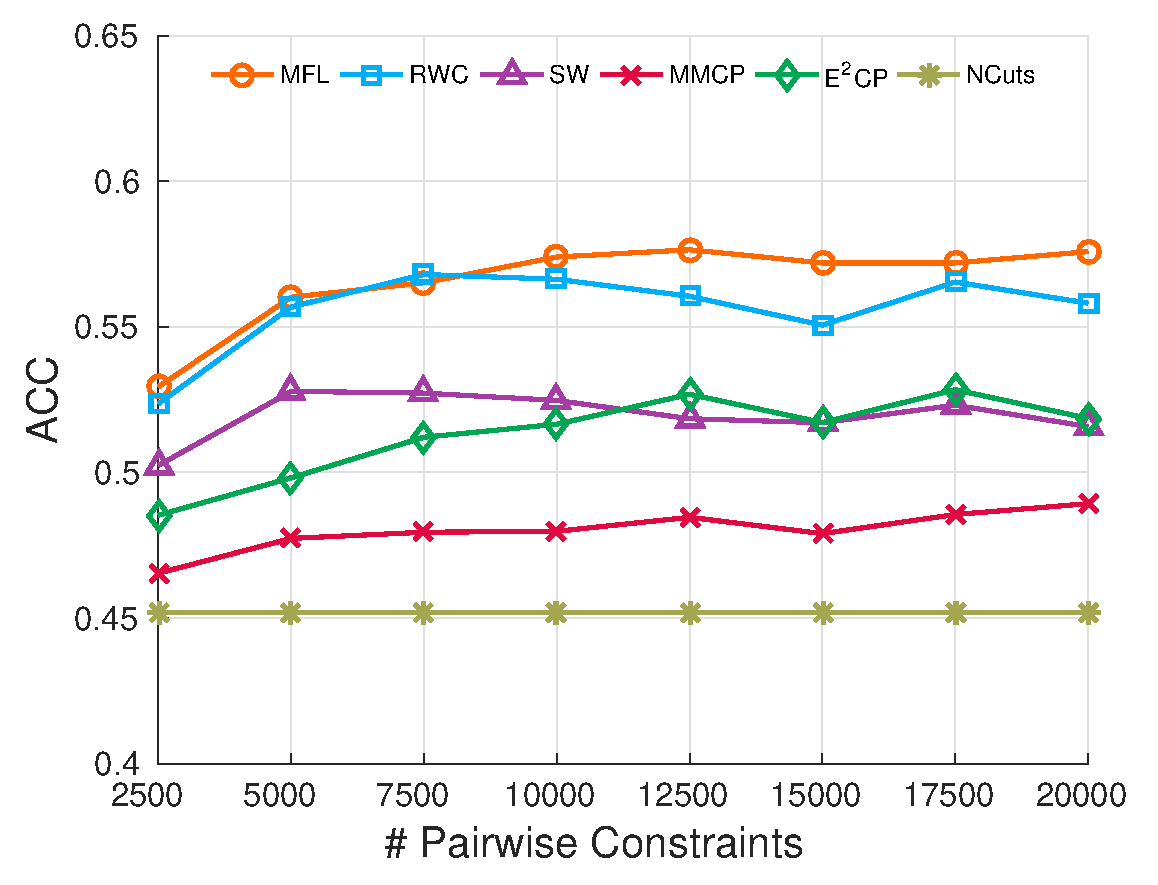
\includegraphics[width=0.495\textwidth]{chap3/corel5k_cn_acc.eps}}
                    \label{fig3:corel5k_cn_acc}
	\bisubcaptionbox{Corel 5k数据集上的NMI结果}%
					{NMI on  Corel 5k}
                    [0.495\textwidth]{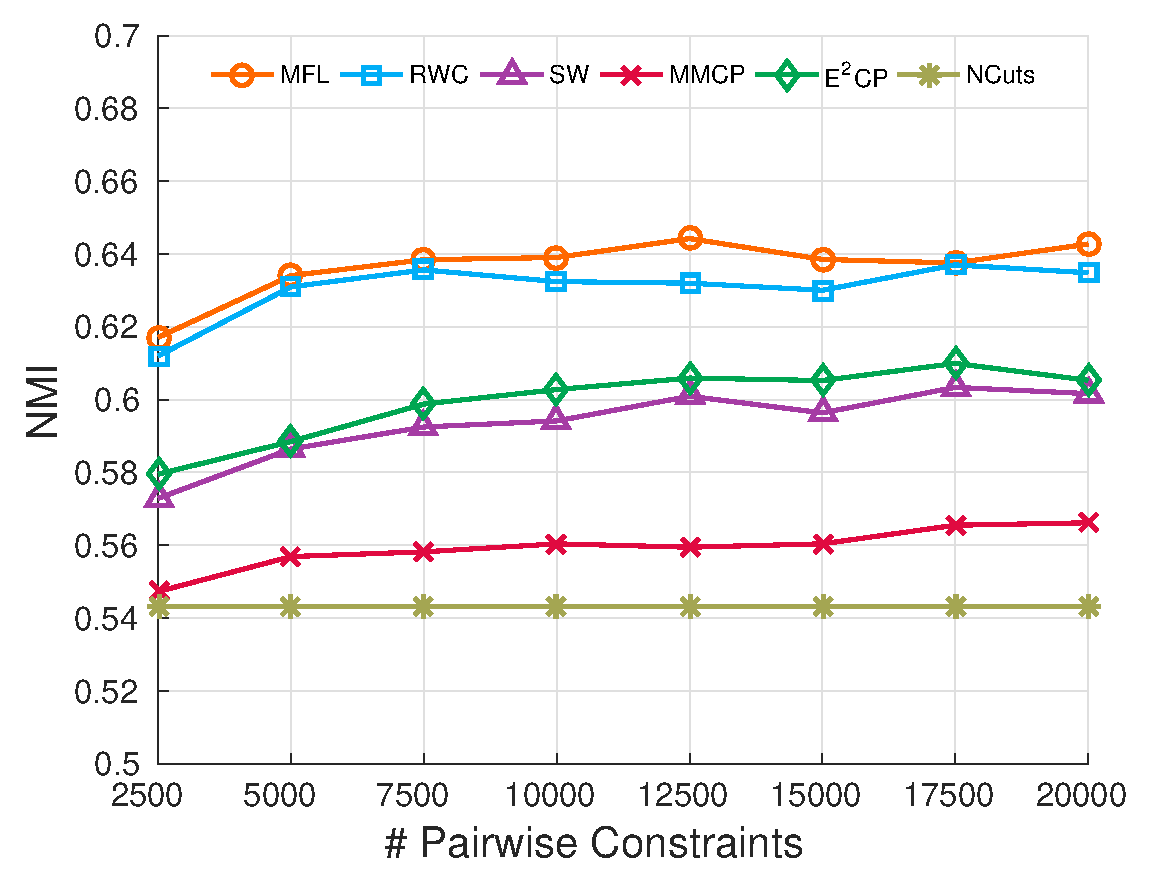
\includegraphics[width=0.495\textwidth]{chap3/corel5k_cn_nmi.eps}}
                    \label{fig3:corel5k_cn_nmi}
                    
	\centering
	\bisubcaptionbox{PASCAL VOC'07数据集上的ACC结果}%
					{ACC on  PASCAL VOC'07}
					[0.495\textwidth]{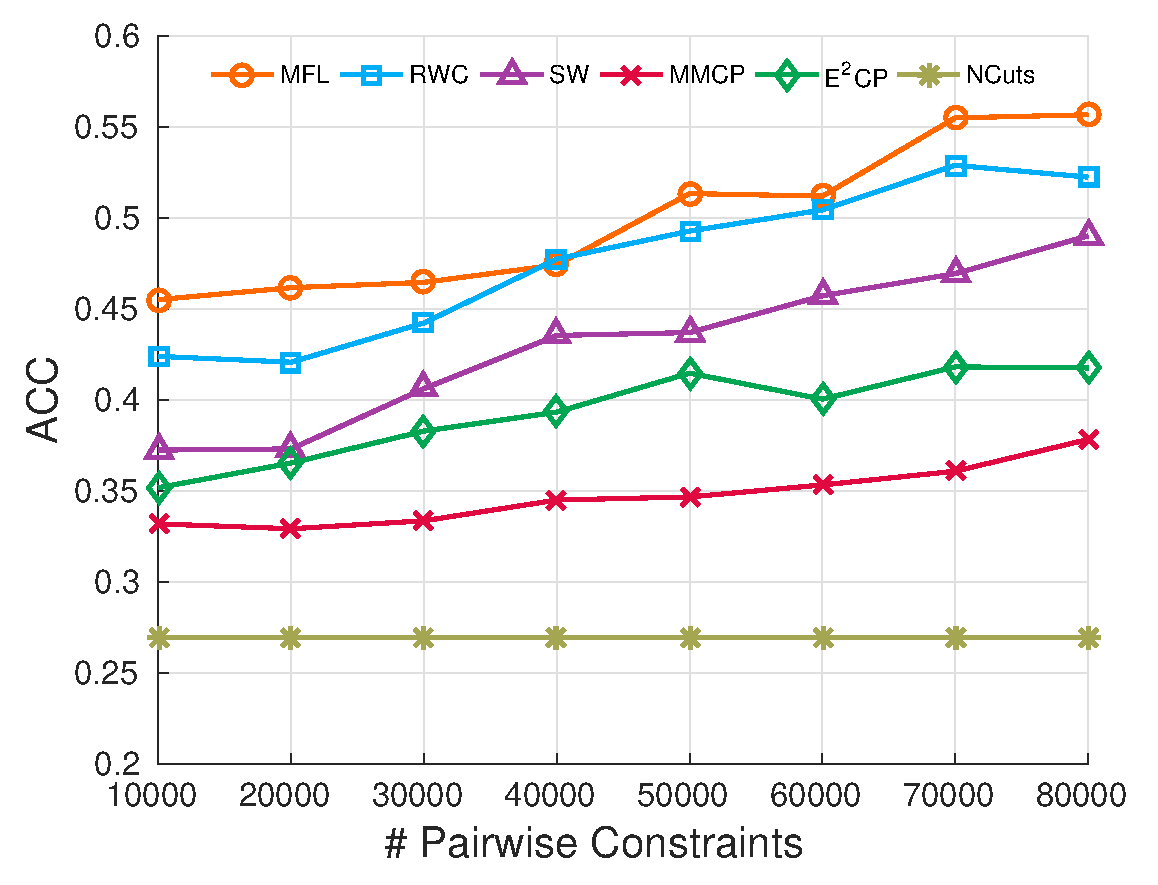
\includegraphics[width=0.495\textwidth]{chap3/voc_cn_acc.eps}}
                    \label{fig3:voc_cn_acc}
	\bisubcaptionbox{PASCAL VOC'07数据集上的NMI结果}%
					{NMI on  PASCAL VOC'07}
					[0.495\textwidth]{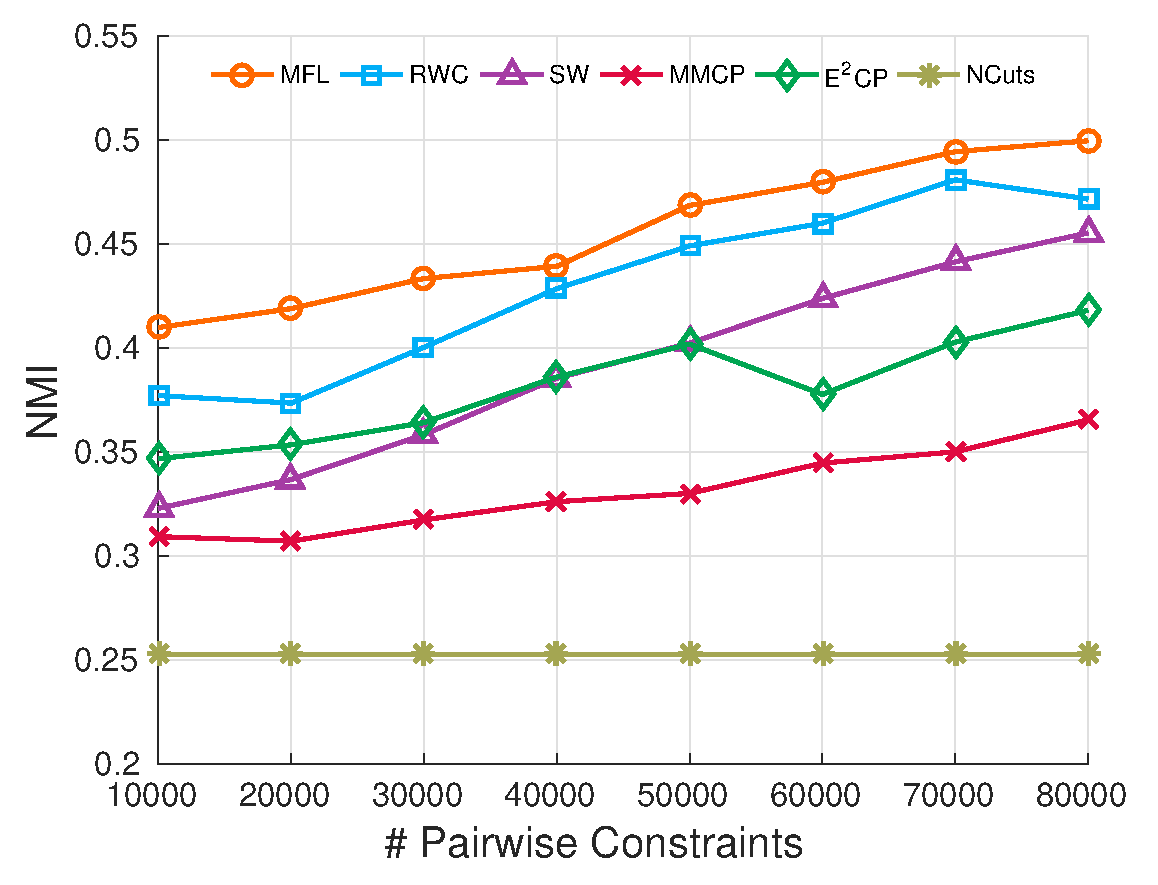
\includegraphics[width=0.495\textwidth]{chap3/voc_cn_nmi.eps}}
                    \label{fig3:voc_cn_nmi}
	\bicaption{在Corel 5k和PASCAL VOC'07数据集上,不同约束数量下采用3个模态的聚类效果}{Clustering performance of 3 modalities on Corel 5k and PASCAL VOC'07 with different numbers of  constraints}
	\label{fig3:cn}
\end{figure} 


\begin{figure}[t]
	\centering
	\bisubcaptionbox{Corel 5k数据集上的ACC结果}%
					{ACC on  Corel 5k}
					[0.495\textwidth]{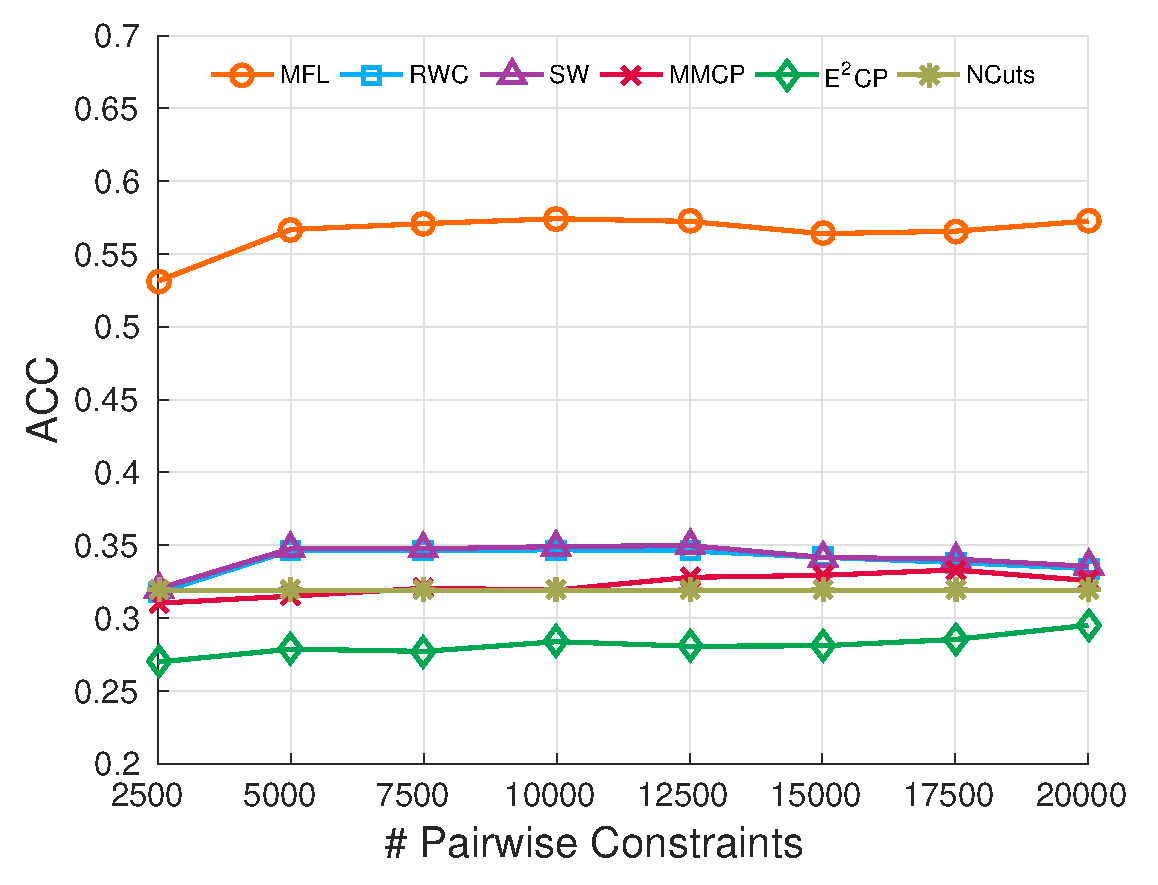
\includegraphics[width=0.495\textwidth]{chap3/corel5k_cn_16_acc.eps}}
                    \label{fig3:corel5k_cn_16_acc}
	\bisubcaptionbox{Corel 5k数据集上的NMI结果}%
					{NMI on  Corel 5k}
                    [0.495\textwidth]{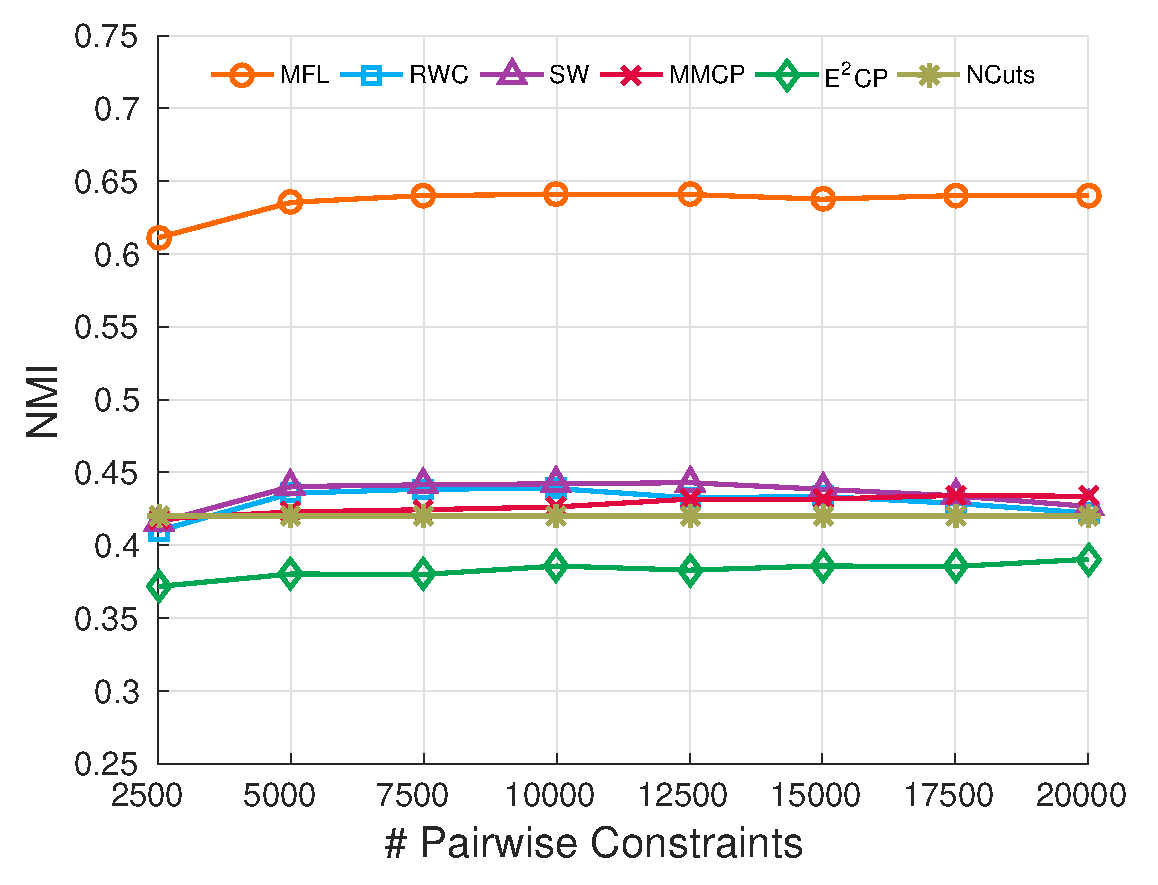
\includegraphics[width=0.495\textwidth]{chap3/corel5k_cn_16_nmi.eps}}
                    \label{fig3:corel5k_cn_16_nmi}
                    
	\centering
	\bisubcaptionbox{PASCAL VOC'07数据集上的ACC结果}%
					{ACC on  PASCAL VOC'07}
					[0.495\textwidth]{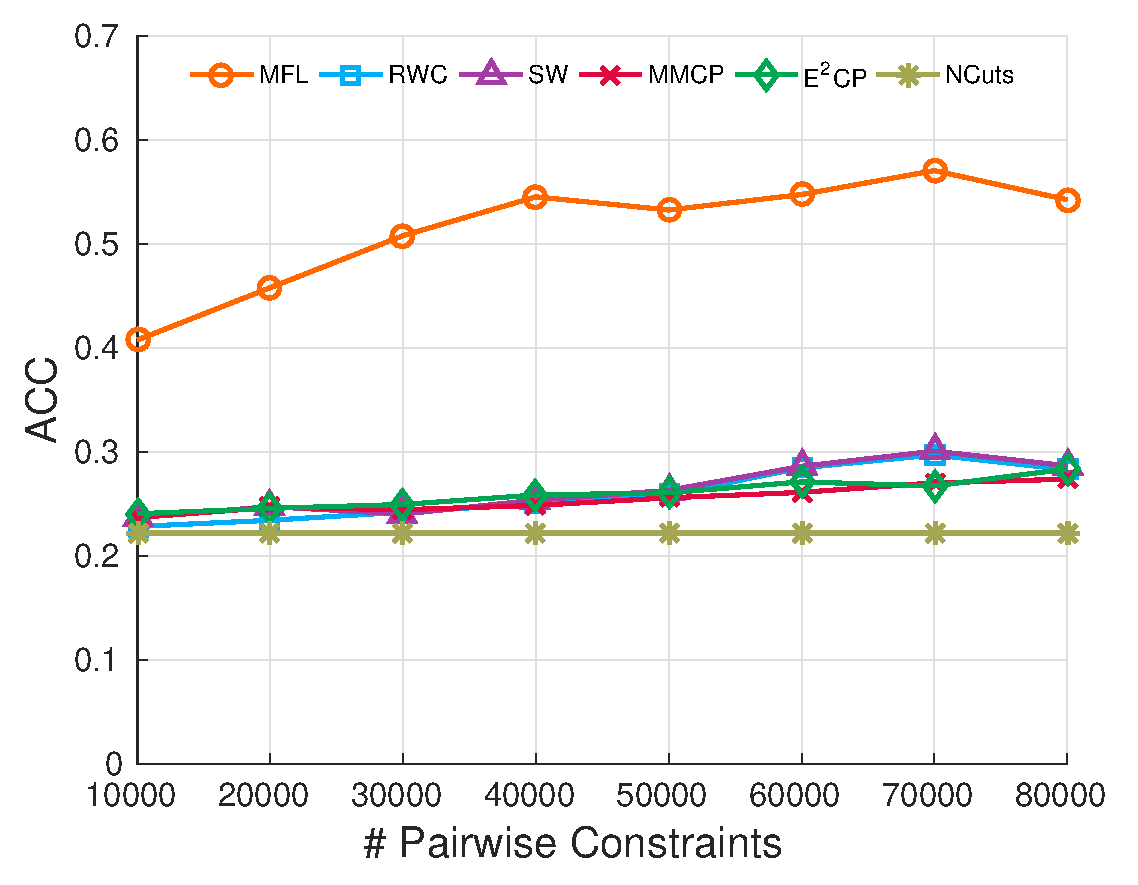
\includegraphics[width=0.495\textwidth]{chap3/voc_cn_16_acc.eps}}
                    \label{fig3:voc_cn_16_acc}
	\bisubcaptionbox{PASCAL VOC'07数据集上的NMI结果}%
					{NMI on  PASCAL VOC'07}
					[0.495\textwidth]{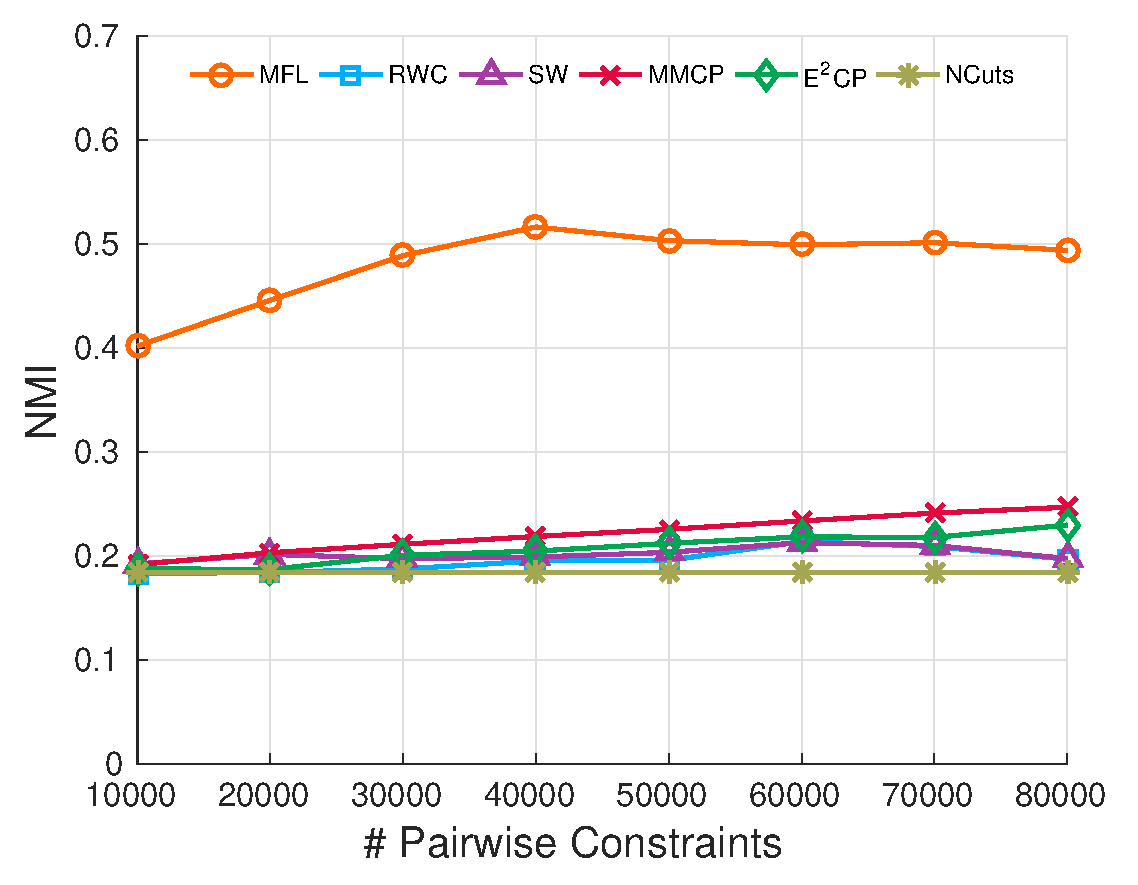
\includegraphics[width=0.495\textwidth]{chap3/voc_cn_16_nmi.eps}}
                    \label{fig3:voc_cn_16_nmi}
	\bicaption{在Corel 5k和PASCAL VOC'07数据集上,不同约束数量下采用16个模态的聚类效果}{Clustering performance of 16 modalities on Corel 5k and PASCAL VOC'07 with different numbers of  constraints}
	\label{fig3:cn_16}
\end{figure} 

与Corel 5k数据集不同,PASCAL VOC'07数据集是为目标检测而提出的多标签数据集。该数据集中的许多数据样本都在真实标签中被标注了多个类别。我们在PASCAL VOC'07数据集上采用了一个标注技巧,而不是多标签聚类方法,以使其评测指标与在Corel 5k上的聚类结果保持一致可比较。
我们将每个多标签数据样本复制多次以生成与其标签数量一样多的相同样本。然后,为每个副本分配一个标签。因此,带有$ t $个标签的数据样本将变成$ t $个分别仅带有一个标签的不同样本,尽管这些样本都有相同的特征。使用这种多标签增强技巧后,性能测度ACC和NMI将始终小于1。因此,我们将评估结果除以理想化最优结果,以对评估分数进行归一化。

\subsection{性能评估与比较}
在本节中,我们报告并讨论了所提出的MFL和RWC方法以及对照算法的聚类性能。为了将我们的方法与专门针对两种模态所设计的方法进行比较,我们设计了两种模态下的聚类实验。我们选择\textit{DenseSift}和\textit{tags}两种模态,并在表\ref{tab3:2modal}中展示了不同算法的聚类性能。我们选取成对约束总数的$0.08\%$作为观测到的成对约束信息,即在Corel 5k数据集上观察到的成对约束的数量为20,000对,在PASCAL VOC'07上观察到的约束的数量是80,000对。在以下实验中,我们采用相同数量的成对约束。从表\ref{tab3:2modal}中我们可以观察到,在Corel 5k数据集上,MFL和RWC表现出了相似的性能,并且胜过其他方法,而在PASCAL VOC'07上,SW方法的结果取得了最佳性能。这是由于\textit{DenseSift}和\textit{tags}两中特征的理想权重可能近似相等。但是,MFL和RWC方法的评估指标仍可与SW相媲美。此外,我们所提出的MFL并非专门针对两种模态情况设计,它旨在解决具有任何数量模态的权重学习问题。MFL仅为每个模态提供一个粗略的先验权重估计,权重估计的质量在很大程度上取决于观察到的约束矩阵$ {Y} $的质量。由于MFL是从约束矩阵$ {Y} $和稀疏相似性矩阵${W}_s $中学习权重,因此较少的模态将导致基矩阵$ {S} $存在大量的全零行,观察到的约束信息无法得到充分利用。如果我们有更多的模态或更多观察到的约束,则权重系数的预测将更加准确。这里需要注意的是,MSCP方法与UCP方法在约束传播后无法生成统一的相似性矩阵,即分别保留了经过约束传播的两个模态的相似性矩阵。因此在实验中我们对这两个相似性矩阵分别聚类,并在表\ref{tab3:2modal}种报告了聚类结果的平均值。

此外,我们在更多的模态上进行了实验,并选择了三种不同的情况:3、8和16种模态。 在3种模态的情况下,我们将\textit{Lab}特征添加到前文所述的2种模态情况下。在8种模态的实验中,我们采用的特征为:\textit{DenseSift,Lab,tags,Hsv,Gist,RgbV3H1,HsvV3H1,HarrisSiftV3H1}。在16种模态的情况下,我们使用了INRIA特征数据集中的所有描述子。在表\ref{tab3:modal_corel}中我们展示了在Corel 5k数据集上的聚类结果,表\ref{tab3:modal_voc}显示了PASCAL VOC'07数据集上相应的聚类结果。从表\ref{tab3:modal_corel}和表\ref{tab3:modal_voc}中可以看出,随着模态数量的增加,提出的MFL算法的优越性变得愈加明显。当考虑到8或16种模态时,绝大多数对照方法都无法处理如此数量众多的模态。因此,我们能看出它们的性能出现明显的下降。

\begin{figure}[t]
    \centering
    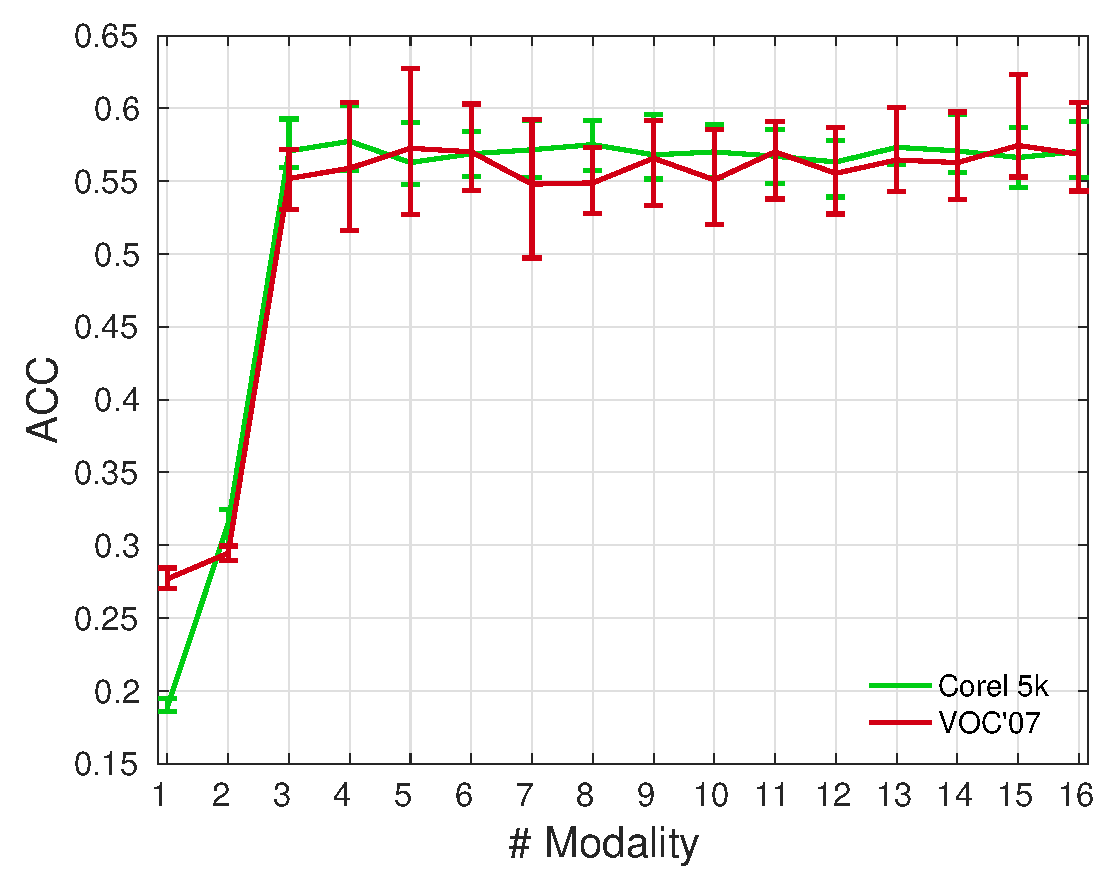
\includegraphics[width=0.495\textwidth]{chap3/corel5k_voc_1_16_acc.eps}
    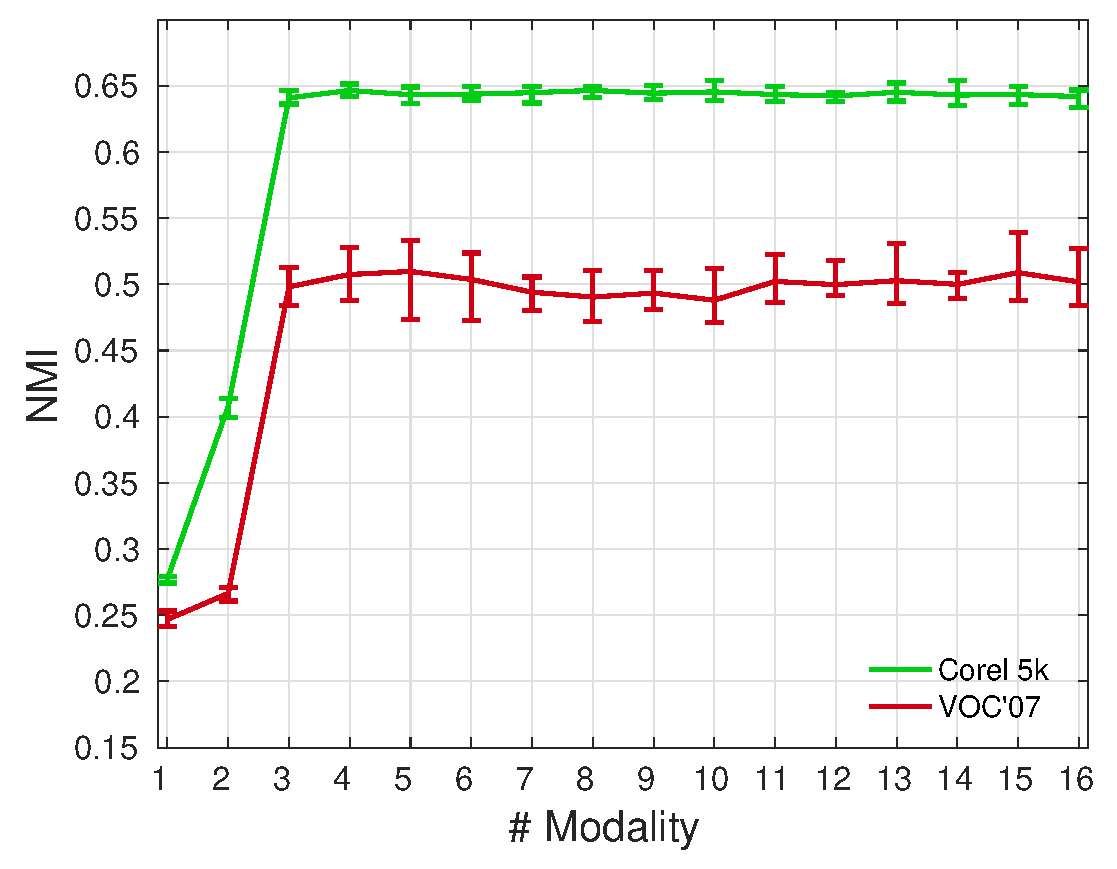
\includegraphics[width=0.495\textwidth]{chap3/corel5k_voc_1_16_nmi.eps}
	\bicaption{在不同数量模态上的聚类结果}{Clutering results with different number of modalities}
	\label{fig3:1_16}
\end{figure} 

在图\ref{fig3:cn}和图\ref{fig3:cn_16}中,我们展示了在3种和16种模态下,使用不同数量的成对约束的聚类效果。如前所述,由于MCMCP所需时间代价极大,本实验不涉及MCMCP方法,通过表\ref{tab3:2modal},表\ref{tab3:modal_corel}和表\ref{tab3:modal_voc}足以显示MCMCP的聚类性能。根据图\ref{fig3:cn}所显示的聚类结果,对于3种模态的情况,MFL方法在不同数量成对约束的设置下的聚类效果均优于其他方法,这种优势在图\ref{fig3:cn_16}所展示的实验结果中变得更加明显。


正如在第\ref{sec3:dis}节中所论述的,我们在图\ref{fig3:1_16}中研究了所提出的MFL算法的模态选择能力。在本实验中,通过将每种模态依次增添到MFL方法,以测试在不同数量模态的情况下MFL的聚类性能。选择的顺序为\textit{DenseSift,Lab,tags,Hsv,Gist,RgbV3H1,HsvV3H1,HarrisSiftV3H1,HarrisSift,HarrisSiftV3H1,DenseSiftV3H1,DenseHue,HarrisSift,HarrisHue,HarrisHueV3H1,Rgb}。可以注意到,当\textit{tags}特征被添加到MFL方法中时,聚类性能会显著地提高,然后效果近似达到饱和状态。这是因为文本描述特征本身包含了更多的具有判别性能力的信息,并且在\textit{tags}之后添加的特征只能提供一些冗余的信息。值得注意的是,每个模态都包含一些判别性信息以及噪声信息。如果新的模态无法提供非冗余信息,则额外引入的噪声将导致聚类性能下降。这也可以解释为什么大多数对照算法无法处理极其多种模态。与之相反的是,在MFL中,当不断增加模态数量时,权重的稀疏性将消除冗余的和不具有判别力的模态,从而保持鲁棒性。

为了进一步证明MFL算法可以帮助进行模态选择,仿照图\ref{fig3:1_16}的实验设置,以图\ref{fig3:1_16_more}来展示所提出的MFL在Corel 5k数据集上对于四种不同添加顺序的模态序列的聚类结果。图\ref{fig3:1_16_acc_nmi_4}所展示的模态添加顺序为\textit{tags,HarrisHueV3H1,Gist,DenseSiftV3H1,RgbV3H1,HsvV3H1,LabV3H1,DenseHueV3H1,HarrisSiftH3V1,Hsv,HarrisHue,DenseSift,HarrisSift,Lab,DenseHue,Rgb}。图\ref{fig3:1_16_acc_nmi_5}显示了图\ref{fig3:1_16_acc_nmi_4}中添加顺序的逆序的聚类结果,该序列以\textit{HarrisHueV3H1}和\textit{tags}作为结尾。图\ref{fig3:1_16_acc_nmi_6}的模态顺序为\textit{tags,DenseSift,Gist,LabV3H1,RgbV3H1,HsvV3H1,DenseSiftV3H1,DenseHueV3H1,HarrisSiftV3H1,Hsv,HarrisHue,HarrisHueV3H1,DenseHue,Rgb,HarrisSift,Lab}。图\ref{fig3:1_16_acc_nmi_7}显示了图\ref{fig3:1_16_acc_nmi_6}中添加顺序的逆序的聚类结果,该序列以\textit{DenseSift}和\textit{tags}结尾。可以注意到,在以\textit{tags}起始的图\ref{fig3:1_16_acc_nmi_4}和图\ref{fig3:1_16_acc_nmi_6}中,仅使用一种或两种模态信息,所取得的聚类性能已经非常出色。这是因为\textit{tags}是文本描述信息,比视觉描述更具有判别性。在向序列中添加更多的模态后,由于来自视觉描述特征的附加信息,实验结果得到了$2\%$的性能改进。而在多数实际应用中,文本描述是一种从用户处收集代价较高的特征。我们更进一步地在图\ref{fig3:1_16_acc_nmi_5}和图\ref{fig3:1_16_acc_nmi_7}中展示以\textit{tags}作为结束的模态序列的聚类效果。尽管\textit{tags}能够产生可观的性能改进,但是聚类性能依然受益于持续增加的视觉特征数量。如果没有文本描述,在仅使用15种模态的情况下,所提出的MFL算法在仅用一种或两种模态的基础上,大约可提高$10\%$的聚类性能。

\begin{figure}[t]
	\centering
	\begin{subfigure}{0.495\textwidth}
		\centering
		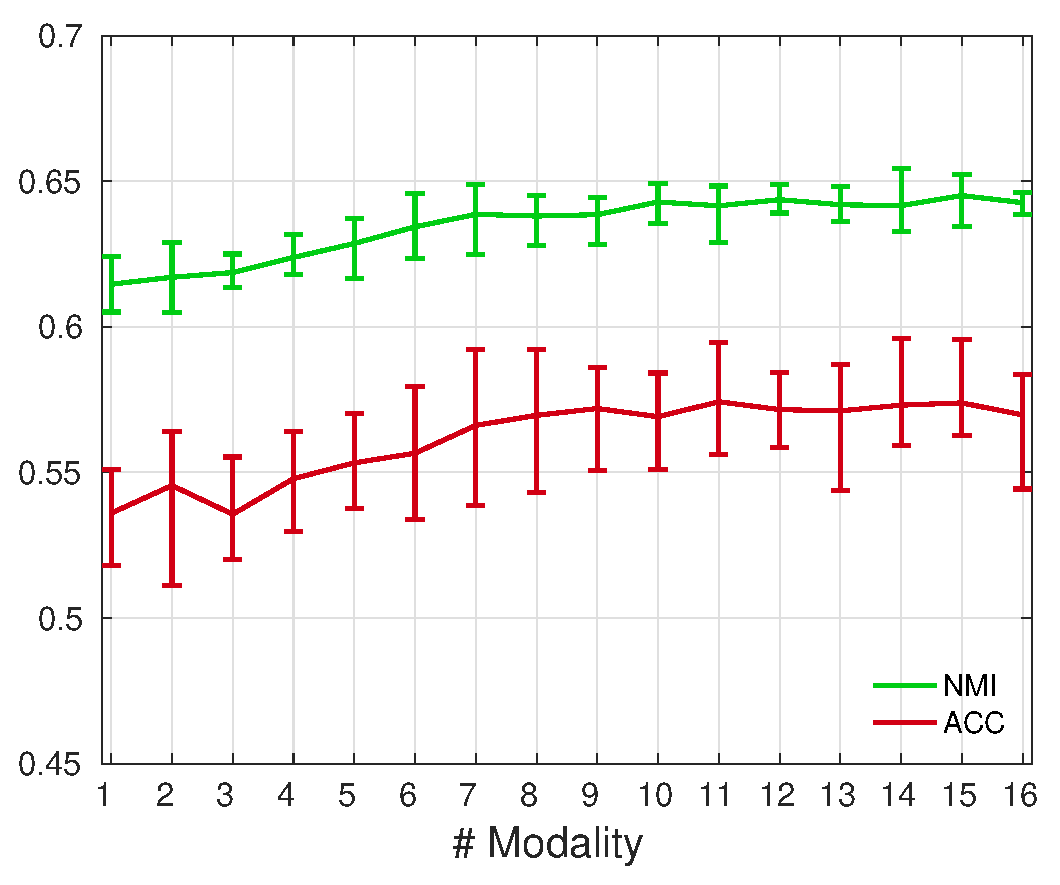
\includegraphics[width=\textwidth]{chap3/corel5k_1_16_acc_nmi_4.eps}
		\caption{}
		\label{fig3:1_16_acc_nmi_4}
	\end{subfigure}
	\begin{subfigure}{0.495\textwidth}
		\centering
		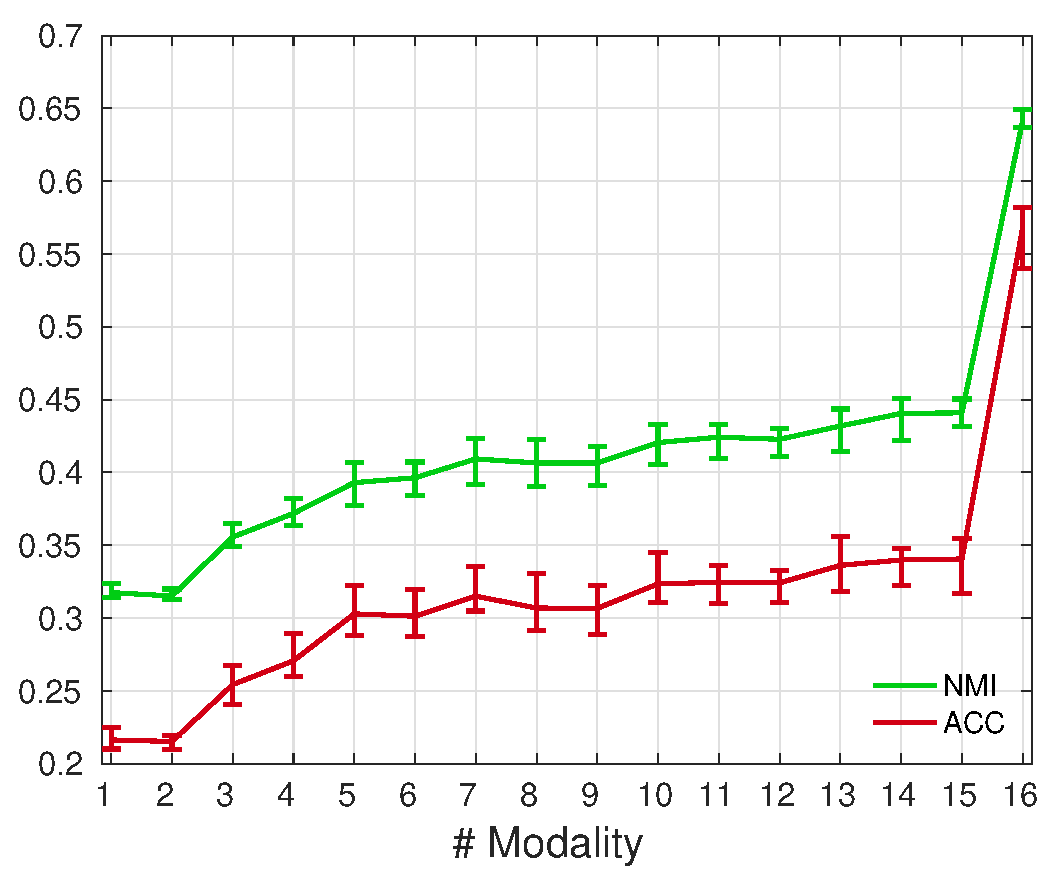
\includegraphics[width=\textwidth]{chap3/corel5k_1_16_acc_nmi_5.eps}
		\caption{}
		\label{fig3:1_16_acc_nmi_5}
    \end{subfigure}
    
	\centering
	\begin{subfigure}{0.495\textwidth}
		\centering
		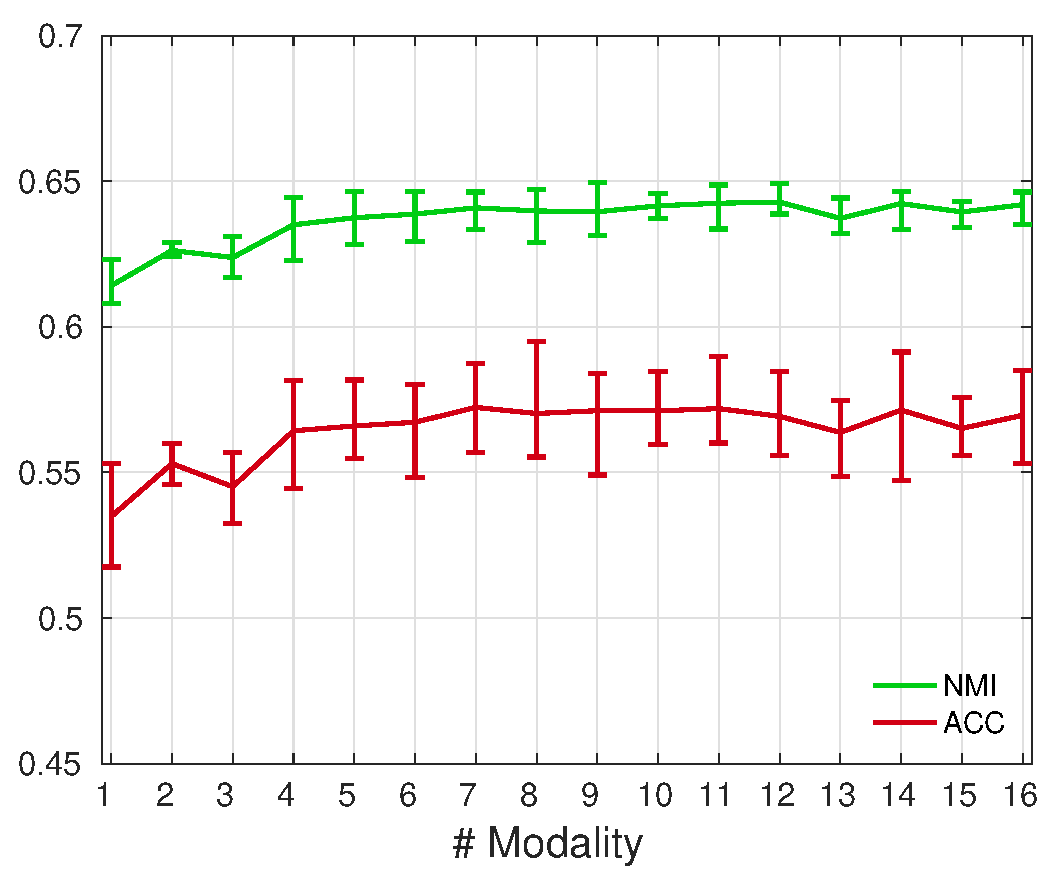
\includegraphics[width=\textwidth]{chap3/corel5k_1_16_acc_nmi_6.eps}
		\caption{}
		\label{fig3:1_16_acc_nmi_6}
	\end{subfigure}
	\begin{subfigure}{0.495\textwidth}
		\centering
		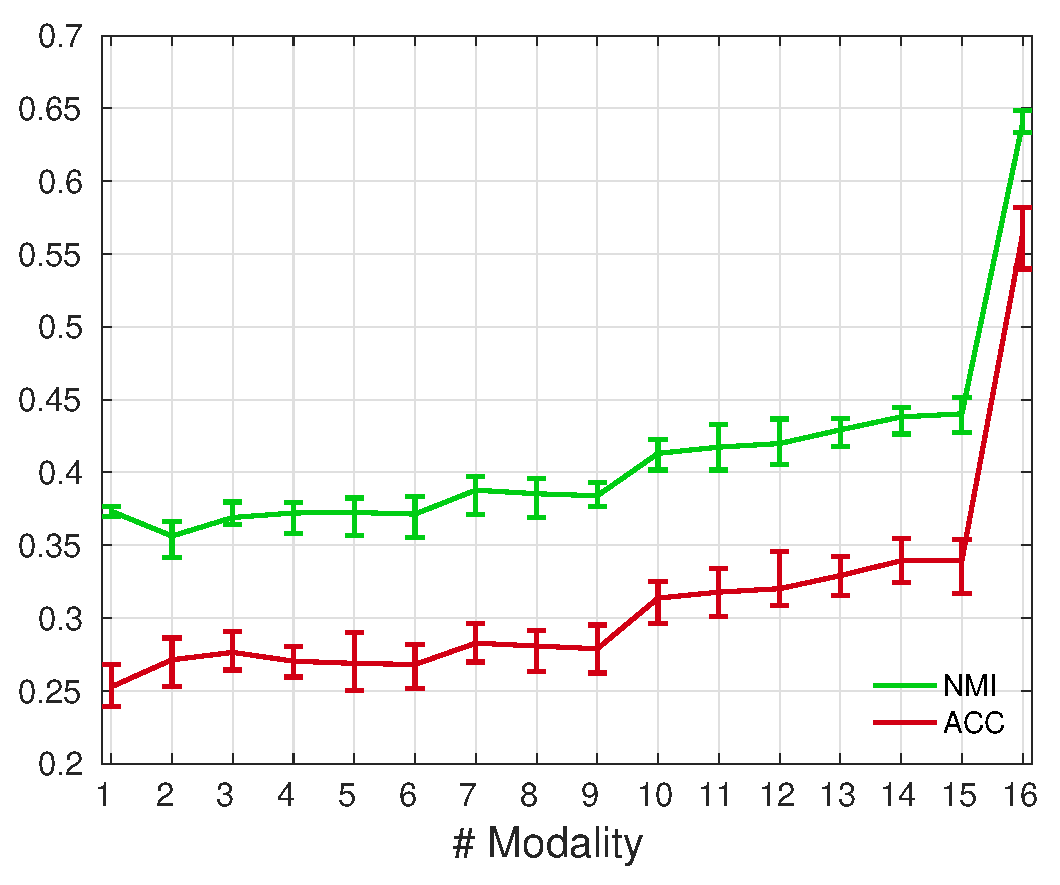
\includegraphics[width=\textwidth]{chap3/corel5k_1_16_acc_nmi_7.eps}
		\caption{}
		\label{fig3:1_16_acc_nmi_7}
	\end{subfigure}
	\bicaption{在Corel 5k数据集上不同模态顺序的聚类效果。a)以特征 \textit{tags} and \textit{HarrisHueV3H1}作为起始的模态序列;b)序列a)的逆序列;c)以特征 \textit{tags} and \textit{DenseSift}作为起始的模态序列;d)序列c)的逆序列}{Clutering results with different orders of modalities on Corel 5k. a) Modality sequence starts with \textit{tags} and \textit{HarrisHueV3H1}; b) Inverse order of a); c) Modality sequence starts with \textit{tags} and \textit{DenseSift}; d) Inverse order of c)}
    \label{fig3:1_16_more}
\end{figure}

\section{本章小结}
在本章中,我们将多标签传播中广泛使用的RWC方法通过近似的方式引入了多模态约束传播问题。更进一步地,本章提出了一种在多模态约束传播中的新颖的融合学习方法,称为多模态融合学习(Multi-modal Fusion Learning,MFL)。MFL方法从所观察到的成对约束的重建损失以及传播过程中学习模态的相似性融合。此外,本章还讨论了不同的算法在极多数量的模态下的承压能力,并通过大量实验结果证明了所提出方法的优越性。
% !TEX root = ../thesis.tex
\chapter{基于相容条件概率分布重构的相似性学习}
\section{引言}
如前文所述,约束传播方法多数为针对单模态情况而设计的。近年来,有大量的工作对多模态融合进行了深入的研究\cite{lahat2015multimodal,poria2017ensemble,yu2017deep,poria2017review,liu2018weakly,kiela2018efficient}。在无监督或半监督的多模态任务中,学习的核心阻碍是训练数据不足而难以学习不同模态的权重。
模态权重表示了每种模态的重要性,因此,一些工作主张如果我们可以获得关于模态的先验知识,则可以为噪声较大的模态分配较小的权重\cite{kumar2011co,liu2013multi}。

在前文中我们所提出的MFL算法将模态级的融合学习推广到了多模态约束传播问题中。但是,通常情况下从模态的鲁棒性推导得出模态权重是更加合理。Sohn等人提出了一种深度学习方法以最小化两种模态之间的信息差异\cite{sohn2014improved},这可以视为通过鲁棒性学习模态融合的特殊情况。同时在鲁棒相似性矩阵学习方面也取得了一些进展\cite{pavan2007dominant,premachandran2013consensus,zhu2014constructing}。这些方法
提供了不同的标准来衡量每个模态信息是否有噪声,而我们可以利用这些方法来生成模态的一些先验知识。

在本文中,我们首先提出并解决了相容条件概率分布重构(Compatible Conditional Distributions Reconstruction,CCDR)这个基础问题。基于CCDR,我们设计了一种新的多模态约束传播相似性学习方法,被命名为实例级多模态约束传播(Instance Level Multi-Modal Constraint Propagation,ILMCP)。
ILMCP会根据从每个模态上学习到的实例级的鲁棒性,为约束传播生成出统一的相似性图。所提出的方法将关注点集中在多模态约束传播中的转移概率推理上。
此外,区别于先前的工作,我们在本章所提出的方法建立在数据实例的邻域鲁棒性上,而不是每个模态整体的稳健性。为此,我们在算法中对一对相容条件概率分布进行了重构,即给定特定数据实例条件下的模态概率以及给定某个模态条件下的特定数据实例的概率。随后,我们从上述分布中得出统一的转移概率,以生成一个相似性矩阵。除此之外,我们引入了一种代价敏感(cost-sensitive)的方法来平衡传播过程中的正约束和负约束数量问题。在数学符号表示上我们将延续上一章中的设定。

\section{相容条件概率分布重构}
在本节中,我们提出在特定假设下条件概率相容的必要和充分条件,并提出用于相容条件概率分布重构(Compatible Conditional Distributions Reconstruction,CCDR)的方法。

在许多实际情况下,条件分布比联合分布更加易于直观理解。研究人员更倾向于在提出的方法中采用一组假定存在的条件分布族,例如$P(X|Y)$和$P(Y|X)$\cite{arnold1989compatible}。但是,可能并不存在能够生成特定条件分布族的相关联的边缘概率分布和联合概率分布,这种情况被称为条件概率分布不相容。为了更准确的描述这种情况,我们在下文中给出了相容条件概率分布的定义。

\begin{definition}
    对于两个候选的条件概率分布族$ P(X|Y) $ 和 $ P(Y|X) $,如果存在一个与两者相关联的 $ (X,Y) $的联合概率分布,则称两个候选条件概率分布族为相容,否则称两个候选条件概率分布族不相容。
\end{definition}

条件概率分布相容性的充分必要条件由Arnold等人在文献\parencite{arnold1989compatible}中首次提出。由于文献\parencite{arnold1989compatible}中提出的条件针对于概率分布的一般情况,该条件对两个条件概率分布中随机变量可能取值的任意组合进行了性质讨论。同时上述文献中并未对如何从两个不相容的条件概率分布中重建出相容条件概率分布进行研究。

在假设这些双变量有限离散的条件概率分布中不存在\textbf{零值概率}的情况下,我们给出了更加简洁的相容条件概率分布的充要条件,并给出了一个线性代数角度的证明。

\begin{theorem}
    \label{thm4}
    对于条件概率分布 $P(Y|X)$ 和 $P(X|Y)$,定义商矩阵$Q$,其中${q}_{i,j} = \frac{P(x_i|y_j)}{P(y_j|x_i)}$。$P(Y|X)$ 和 $P(X|Y)$为相容条件概率分布当且仅当商矩阵$Q$为秩$1$矩阵且$\sum_j\frac{1}{\sum_i {q}_{i,j}} = 1$。
\end{theorem}
\begin{proof}
    假设$P(Y|X)$ 和 $P(X|Y)$为相容条件概率分布。则必然能找到相关联的边缘概率分布$P(X), P(Y)$,以及联合概率分布$P(X, Y)$。因此可以得到:
    \begin{equation}
    {q}_{i,j} = \frac{P(x_i|y_j)}{P(y_j|x_i)} = \frac{P(x_i)}{P(y_j)}.
    \label{eq4:q}
    \end{equation}
    给定商矩阵$Q$的第$s$行,则能够通过求$s$行与$\frac{P(x_t)}{P(x_s)}$的乘积确定商矩阵$Q$的第$t$行元素。这导致了$Q$为一个秩$1$矩阵。且通过公式(\ref{eq4:q})可以得到
    \begin{equation}
    \sum_j\frac{1}{\sum_i {q}_{i,j}} = \sum_j\frac{1}{\sum_i \frac{P(x_i)}{P(y_j)}} = \sum_j P(y_j) = 1  
    \end{equation}

    相反地,假设$Q$为一个秩$1$矩阵成立且。则商矩阵$Q$可以被写为两个正向量$m$和$n$的乘积,即$Q = mn^T$。如果假设有$\sum_i  {m}_i = 1$,则能够通过上述分解得到唯一的向量组合$m$和$n$。将${q}_{i,j} ={ m}_i{n}_j$ 带入 $\sum_j\frac{1}{\sum_i {q}_{i,j}} = 1$中,可以得到$\sum_j\frac{1}{{n}_j} = 1$。
    从而可以通过两个正向量$m$和$n$构建两个离散边缘概率分布:
    \begin{equation}
    P(x_i) = {m}_i, \quad P(y_j) = \frac{1}{{n}_j}.
    \end{equation}

    接下来,我们将证明存在能够满足 $P(X, Y) = P(Y|X)P(X) = P(X|Y)P(Y)$的联合概率分布$P(X, Y)$。
    由于$P(Y|X)$ 和 $P(X)$ 分别唯一个条件概率分布和一个边缘概率分布,因此,也可以将两者的乘积视为一个概率分布。相似地,乘积 $P(X|Y)P(Y)$ 也可以构造为一个概率分布。故,存在性证明的核心在于证明 $P(y_j|x_i)P(x_i) = P(x_i|y_j)P(y_j)$ 对于所有的 $i$ 和$j$恒成立。
    基于 ${q}_{i,j} = {m}_i{n}_j$可知
    \begin{equation}
    \begin{split}
    &\frac{P(x_i|y_j)}{P(y_j|x_i)} = {q}_{i,j} = {m}_i{n}_j\\
    \Rightarrow &\frac{P(x_i|y_j)}{{n}_j} = P(y_j|x_i) {m}_i\\
    \Rightarrow &P(x_i|y_j)P(y_j) = P(y_j|x_i)P(x_i), 
    \end{split}
    \end{equation}
    即表明$P(Y|X)$ 和 $P(X|Y)$为两个相容的条件概率分布族。
\end{proof}

基于定理\ref{thm4}我们可以设计出通过两个不相容条件概率分布重建出近似的相容条件概率分布的方法。这里需要注意的是,我们将通过概率$P^\dagger (x_i|y_j)$ 和 $P^\dagger (y_j|x_i)$中的上标$\dagger$ 来表示相应的条件概率分布$P^\dagger (X|Y)$ 和  $P^\dagger (Y|X)$是不相容的。

从定理\ref{thm4}中可以注意到如果希望概率分布$P^\dagger (X|Y)$ 和  $P^\dagger (Y|X)$是相容的,并能够从中推导出概率$P(x_i), P(y_j)$,则需要商矩阵$Q$为秩$1$矩阵。这里我们将暂时忽略条件$\sum_j\frac{1}{\sum_i {q}_{i,j}} = 1$,该条件可以在求解后通过缩放重新满足。一般情况下,矩阵$Q$不会为秩$1$矩阵。一个可能的解决方案为假设不相容分布$P^\dagger (X|Y)$ 和  $P^\dagger (Y|X)$在观测中受噪声干扰,其真实分布为相容条件概率分布,并且含有噪声的商矩阵$Q$接近秩$1$矩阵。

在下文中,我们假设$P^\dagger(X|Y)$ 和 $P^\dagger(Y|X)$ 分别受到高斯噪声$ \mathcal{N}(0, \alpha^2) $ 和  $ \mathcal{N}(0, \beta^2) $的干扰。因此,我们通过对矩阵$Q$进行奇异值分解得到其秩为$1$的近似矩阵$\hat{{Q}}$。目标相容概率分布 $P(X|Y)$ 和  $P(Y|X)$可以通过求解在近似商矩阵$\hat{{Q}}$约束下的极大似然估计求得。最大化对数似然的优化问题可写为:
\begin{equation}
\begin{split}
\mathop{\mathrm{min}}_{P(x_i|y_j), P(y_j|x_i)} & \quad \frac{1}{2 \alpha^2} \sum_{i,j}(P(x_i|y_j)-P^\dagger(x_i|y_j))^2 \\
&+ \frac{1}{2 \beta^2} \sum_{i,j}(P(y_j|x_i)-P^\dagger(y_j|x_i))^2\\
\mathrm{s.t.}\quad \quad \quad&\quad \frac{P(x_i|y_j)}{P(y_j|x_i)} = \hat{{q}}_{i,j}\\
%             &\quad \;\sum_{s}P(u_i|\mathcal{G}_s) = 1\\
%             &\quad \;\sum_{s}P(G_s|u_i) = 1
\end{split}
\label{eq4:Opt}
\end{equation}

在公式(\ref{eq4:Opt})中我们移除了归一化约束$\sum_{i}P(x_i|y_s) = 1$ 和  $\sum_{j}P(y_j|x_i) = 1$。在这个松弛条件下,该优化问题可以通过逐元素独立计算高效地求解,且归一化流程可以在优化求解后进行。在我们的实现中,高斯噪声的方差选择基于受噪声干扰的条件分布确定。更具体地,令$\alpha^2 = \sum_{i,j}P^\dagger(x_i|y_j)^2$ 且 $\beta^2 = \sum_{i,j}P^\dagger(y_j|x_i)^2$。

\section{实例级多模态约束传播}
在本节中我们将对所提出的基于相容条件概率分布重构的实例级多模态约束传播(ILMCP)方法进行介绍,并对部分实现细节进行描述。
\subsection{模态信息鲁棒性}
在ILMCP中,我们通过近似Consensus $k$-NNs\cite{premachandran2013consensus}的方法对每个模态的鲁棒性进行近似估计。Consensus $k$-NNs方法通过收集多轮$k$-NN近邻的公式信息提供一个可供进行近邻选择的判别标准,该方法可以被看作是二阶相似性(Second-order Proximity)\cite{tang2015line,wang2016structural}的一种近似。如果数据点对$u_i$ 和 $u_j$同时出现在许多其他数据点的$k$-NN近邻中,则该点对相似的可能性更高。反之,如果两个数据点$u_i$和$u_j$从未同时出现在其他数据实例的近邻中,则即使在该点对上观测到高相似性也有比较大的概率为观测噪声。
在算法\ref{alg4:consknn}中我们给出了根据Consensus $k$-NNs构建共识矩阵$C$的算法细节。$C$中的元素可以被用于估计任意两个数据点间的相似性的鲁棒程度。此外,通过在Consensus $k$-NNs中设置阈值$\tau$,可以${c}_{i,j}\le\tau$的任意点对$u_i$和$u_j$互相从对方的近邻集合中移除。
\begin{algorithm}[tb]
    %		\small
            %	\renewcommand{\algorithmicrequire}{\mathbf{Input:}}
            %	\renewcommand{\algorithmicensure}{\mathbf{Output:}}
            \caption{构造共识矩阵}
            \label{alg4:consknn}
            ${C} = \mathbf{0}$;
            \For {$i = 1:N$}{
                \ForAll {$u_j, u_k$满足$u_j, u_k \in \mathcal{N}_k(u_i)$}{
                    % 					 \text{ \AND } j\neq k$}
                    ${c}_{j,k} = {c}_{j,k}+1$\;
                    ${c}_{k,j} = {c}_{k,j}+1$\;
                }
            }
\end{algorithm}

在我们的方法中,共识矩阵的构造与文献\parencite{premachandran2013consensus}中提出的原始算法不同。我们利用共识矩阵从现有的相似性矩阵中对噪声进行剪枝,而不是重建新的近邻集合:
\begin{equation}
{w}^{cons}_{i,j} = 
\begin{cases}
0,\quad\qquad\qquad&\text{if }{c}_{i,j}<\tau;\\ {w}^{dense}_{i,j},&\text{otherwise,}
\end{cases},
\label{eq4:cons}
\end{equation}
这其中,${W}^{dense}$为稠密的$k$NN热力核相似性矩阵,即近邻数量$k$取值较大,我们在实现中令$k = \mathrm{Round}( \frac{\#sample}{\#cluster})$。 ${W}^{cons}$为经过共识矩阵剪枝后的相似性矩阵。由于公式(\ref{eq4:cons})为针对相似性矩阵的一般性公式,不表示某个特定模态,所以我们忽略了矩阵的第三个下标以保持公式的简洁。由于通过$k$-NN近邻构建的矩阵${W}^{dense}$仅是相对稠密的,所以我们的算法实现比原始的Consensus $k$-NNs方法更加高效,在下文中我们将对这一点进行进一步说明。

对于每个模态图$\mathcal{G}_s$,根据公式(\ref{eq4:cons})计算共识相似性矩阵${W}^{cons}_s$。我们对矩阵${W}_s^{dense}$ 和 ${W}_s^{cons}$分别进行行归一化,使得矩阵中的每行可以作为一个概率分布。然后,通过KL散度(Kullback-Leibler divergence)对数据实例在每个模态中的相似性的不一致性(incoherence)进行定义:
\begin{equation}
inc_s(i) = \sum_j {w}^{dense}_{i,j,s}\;\text{ln}\frac{{w}^{dense}_{i,j,s}}{{w}^{cons}_{i,j,s}}, 
\label{eq4:incohere}
\end{equation}
式中${W}^{dense}_{i,j,s}$为数据点对 $u_i$ 和 $u_j$在图$\mathcal{G}_s$上的$k$-NN相似性,${w}^{cons}_{i,j,s}$为相对应的共识相似性取值。

实例级不一致性函数$inc_s(i)$是用于估计图$\mathcal{G}_s$上数据点$u_i$和其近邻间相似性值的鲁棒程度的一个测度。不一致性越小,则说明在数据实例上所观测到的近邻关系越稳定。此外,有两个实现中的细节需要关注。一方面相似性矩阵${W}^{dense}_s$为相对稠密的矩阵。另一方面,我们通过在矩阵 ${W}_s^{dense}$ 和 ${W}_s^{cons}$上叠加一个极小值(例如$10^{-8}$)以解决在离散概率中存在的零值问题。

更进一步地,根据上一章所提出的MFL方法,我们同时定义模态级一致性$ {c}_{mod} = [c_{mod}(\mathcal{G}_1), c_{mod}(\mathcal{G}_2),...] $来描述全局信息:
\begin{equation}
\begin{split}
{c}_{mod} = \;&\mathop{\mathrm{argmin}}_{{c}_{mod}}\; \frac{1}{2}\|{S}{c}_{mod} - {z}  \|_2^2, \\
s.t.\quad&\sum_{s} c_{mod}(\mathcal{G}_s) = 1;\\ &\; c_{mod}(\mathcal{G}_s) \ge 0,
\end{split}
\label{eq4:modalcohere}
\end{equation}
其中$z$为约束向量,$S$为相应的基矩阵, 
\begin{equation}
{S}_{k,s} =  {w}^{dense}_{r(k), c(k), s}, \quad  {z}_k = \begin{cases}1,\quad &\text{if }  {Y}_{r(k),c(k)} =1; \\
0, \quad &\text{otherwise}.
\end{cases}
\end{equation}
函数$ r(i) $返回$Y$中第$i$个约束的行数,$ c(i) $返回相应的列数。

\subsection{统一的多模态相似性学习}
一旦能够求得条件概率$P(\mathcal{G}_s|u_i)$,则可以计算出统一的转移概率$ P(u_i\rightarrow u_j) $。在通过公式(\ref{eq4:modalcohere})和(\ref{eq4:incohere})获取到模态级和实例级的鲁棒性信息后,我们首先根据实例级的不一致性对实例级一致性测度 $ c_s(i) $进行定义,然后给定数据实例$u_i$条件下的图$\mathcal{G}_s$的条件概率则可以通过计算模态级一致性和实例级一致性的归一化乘积得到:
\begin{equation}
c_s(i) = \frac{1}{inc_s(i)+1}
\label{eq4:cohere},
\end{equation}
\begin{equation}
P^\dagger (\mathcal{G}_s|u_i) = \frac{c_s(i) c_{mod}(\mathcal{G}_s)}{\sum_i c_s(i) c_{mod}(\mathcal{G}_s)}
\label{eq4:Pglu}.
\end{equation}

公式(\ref{eq4:cohere})中的定义可以令人联想到t-SNE\cite{maaten2008visualizing}方法中对联合概率的定义形式。而公式(\ref{eq4:Pglu})则基于假设:实例$u_i$在不同模态信息下的不一致性能够反映出不同模态的可信度。具有高可信度的模态可能具有更鲁棒的信息,以及更少的噪声。这里需要注意的是,所计算出的可信度只对应于特定的数据实例$u_i$,因此这属于实例级的可信度。基于该假设,我们需要对概率测度$ P(\mathcal{G}_s|u_i) $进行设计。该概率测度应与不一致性成反比,而相应的最简的构造形式为$ 1/inc_s(i) $。从公式(\ref{eq4:Pglu})中可以发现,在给定模态$s$的情况下,较小的不一致性即隐含了图$\mathcal{G}_s$具有较大的条件概率。在特定情况下,可能出现$ inc_s(i) =0 $的情况,所以我们采用$ inc_s(i) +1 $替代$ inc_s(i)$。因此 $ P(\mathcal{G}_s|u_i) $ 应当正比于 $ (inc_i+1)^{-1} $,而概率公式中的分母项则用于归一化。公式(\ref{eq4:Pglu})为满足该条件的概率测度的最简形式。相应的条件概率$P^\dagger(u_i|\mathcal{G}_s)$可以采用与公式(\ref{eq3:Pulg})相同的方式进行计算。

此处令上文所述的商矩阵中$q_{i,s} = \frac{P^\dagger(u_i|\mathcal{G}_s)}{P^\dagger(\mathcal{G}_s|u_i)}$,通过对矩阵$Q$进行秩$1$近似得到近似矩阵$\hat{Q}$并求解优化问题(\ref{eq4:Opt}),能够得到两个相容条件概率分布的闭式解:
\begin{equation}
\begin{split}
&P(u_i|\mathcal{G}_s) = \frac{\alpha P^\dagger(u_i|\mathcal{G}_s)\hat{{q}}_{i,s}^2+\beta P^\dagger(\mathcal{G}_s|u_i)\hat{{q}}_{i,s}}{\alpha \hat{{q}}_{i,s}^2 + \beta},\\
%             &\quad(\alpha = \frac{1}{\sum_{i,j}P(u_i|\mathcal{G}_j)^2}, \beta = \frac{1}{\sum_{i,j}P(G_j|u_i)^2})\\
&P(\mathcal{G}_s|u_i) = \frac{P(u_i|\mathcal{G}_s)}{\hat{{q}}_{i,s}}\;. 
\end{split}
\label{eq4:OptSlv}
\end{equation}

而由于$\hat{Q}$为近似后的秩$1$商矩阵,边缘概率$P(u_i)$和$P(\mathcal{G}_s)$可以通过分别归一化$\hat{Q}$中的任意一行和任意一列获得,例如:
\begin{equation}
    P(u_i) = \frac{\hat{q}_{i,1}}{\sum_i\hat{q}_{i,1}}, \quad\quad P(\mathcal{G}_s) = \frac{\hat{q}_{1,s}}{\sum_i\hat{q}_{1,s}}.
\end{equation}
相应的根据$\bar{d}_ii=P(u_i)$可以计算出对角权重矩阵$\bar{D}$。

我们可以进一步根据公式(\ref{eq3:mmcp_trans})获得统一的归一化相似性矩阵$\bar{W}$,
\begin{equation}
\begin{split}
\bar{w}_{i,j} &= P(u_i,u_j) \\ &= P(u_i)P(u_i\rightarrow u_j)\\
&=P(u_i)\sum_s P(u_j|u_i, \mathcal{G}_s)P(\mathcal{G}_s|u_i), 
\end{split}
\label{eq4:uni_aff}
\end{equation}
并对该矩阵进行稀疏化。


\subsection{约束传播中的样本不均衡}
需要注意到的是,从数据相似性中采样到的成对约束可能会存在严重的数据分布不均衡问题。 正负约束之间的数量不均衡会在传播后被严重加剧。在本节中我们将从不均衡的二分类角度考虑约束传播问题。更具体地说,我们要将传播的相似性分为两类(即must-link和cannot-link),并控制它们之间的比率。

在不均衡学习上问题有大量的方法先后被提出,两种经典策略:重采样和代价敏感学习仍然在当前的研究工作中占据主导地位\cite{he2009learning,huang2016learning}。考虑到约束信息的稀缺性,我们仅将代价敏感策略引入我们的方法中以解决数据不均衡问题。最近的一些工作显示了在不均衡数据中采用代价敏感学习的优势\cite{shi2000normalized,DBLP:journals/corr/KhanBST15}。

ILMCP方法将约束矩阵$Y$分解成两个矩阵的和的形式${Y} = {Y}_++{Y}_-$,其中${Y}_+$由$Y$中的所有正元素构成:
\begin{equation}
{y}_{+i,j} = 
\begin{cases}
y_{i,j},\quad\qquad\qquad&\text{if }y_{i,j}>0;\\ 0,&\text{otherwise,}
\end{cases},
\end{equation}
相应的${Y}_-$由$Y$中所有的负元素构成。
可以证明,有${Y}_+^T{\bar{{D}} Y}_- = \mathbf{0}$。然后,通过展开 $ \mathrm{tr}(({F}_v - {Y} )^T{\bar{D}}({F}_v - {Y})) $可以得到
\begin{equation}
\begin{split}
\mathrm{tr}((F_v - Y )^T\bar{D}(F_v - Y))=\;&\mathrm{tr}(({F}_v-{Y}_+)^T{\bar{D}}({F}_v-{Y}_+))+\mathrm{tr}(({F}_v-{Y}_-)^T{\bar{D}}({F}_v-{Y}_-))\\
&-\mathrm{tr}({F}_v^T{\bar{D} F}_v). 
\end{split}
\label{eq4:fpif2}
\end{equation}

通过对公式(\ref{eq4:fpif2})的正元素部分增加权重参数$\alpha$,可以将该公式近似看作是一个代价敏感问题。基于文献\parencite{elkan2001foundations}中所提出的定理,如果参数$\alpha$被设置为must-link和cannot-link数量的比值,则可以近似解决样本不均衡的问题。事实上,最理想情况是这两种约束在采样得到的约束矩阵$Y$和转移概率矩阵$F$中有相同的数量比例,而不是令生成的转移概率矩阵$F$中两类约束数量近似相同以完全解决不均衡情况。因此,本方法对不均衡情况的加剧($\alpha=1$)和缓解($\alpha= \frac{\#\text{cannot-link}}{\#\text{must-link}}$)进行了折衷,最终选取权重参数为
\begin{equation}
    \alpha = \sqrt{\frac{\#\text{cannot-link}}{\#\text{must-link}}}.
\end{equation}

将加权后的约束、求解出的相似性矩阵$\bar{W}$,代入回公式(\ref{eq3:MMCP-v})可以得到优化目标函数:
\begin{equation}
\begin{split}
\mathop{\mathrm{min}}_{{F}_v}\;&\frac{1}{2}\alpha\eta \mathrm{tr}(({F}_v-{Y}_+)^T{\bar{D}}({F}_v-{Y}_+))+\frac{1}{2}\eta \mathrm{tr}(({F}_v-{Y}_-)^T{\bar{D}}({F}_v-{Y}_-))\\
&+\frac{1}{2}\mathrm{tr}({F}_v^T(\bar{L}-\eta {\bar{D}}){F}_v), 
\end{split}
\label{eq4:obj2}
\end{equation}
其中$\bar{L} = \bar{D} - \bar{W}$。通过令目标函数关于$F_v$的导数等于零求解该优化问题,能够获得公式(\ref{eq3:sol-v})形式相似的竖直方向传播结果矩阵$F_v$:
\begin{equation}
\begin{split}
        & \alpha\eta \bar{D} (F_v - Y_+) + \eta\bar{D} (F_v - Y_-)+(\bar{L}-\eta\bar{D})F_v = 0\\
% \Rightarrow  \;           & (\alpha+1)\eta \bar{D} F_v - \eta\bar{D}(\alpha Y_+ + Y_-) + (\bar{L}-\eta\bar{D})F_v = 0\\
\Rightarrow   \;          & (\bar{L}+\alpha\eta\bar{D})F_v = \eta\bar{D}(\alpha Y_++Y_-)\\
\Rightarrow   \;          & {F}_v = \eta(\bar{L}+\alpha\eta{\bar{D}})^{-1}{\bar{D}}(\alpha {Y}_++{Y}_-),
\end{split}
\end{equation}
同样的方法也能够求得水平方向传播结果$F_h$。此后,通过合并竖直和水平方向的传播结果可以得到最终的传播结果矩阵$F$:
\begin{equation}
{ F} = \eta^2(\bar{L}+\alpha\eta{\bar{D}})^{-1}{\bar{D}}(\alpha {Y}_++{Y}_-){\bar{D}}(\bar{L}+\alpha\eta{\bar{D}})^{-1}.
\end{equation}


\begin{algorithm}[tb]
	\SetKwInput{KwIn}{输入}
    \SetKwInput{KwOut}{输出}
    \caption{ILMCP算法流程}
    %	\caption{Instance Level Multi-Modal Constraint Propagation}
    \label{alg4:ilmcp}
    \KwIn{稠密 $ k $-NN 相似性矩阵 ${W}_s^{dense}$;约束矩阵 $ {Y} $;聚类数量 $c$;共识矩阵阈值$ \tau $.}
    \KwOut{Sigmoid 相似性矩阵 $ {W^*}$.}
    根据公式(\ref{eq4:cons}}为每个模态构建共识相似性矩阵$ {W} ^{cons}_s$;\\
    根据公式(\ref{eq4:modalcohere})、(\ref{eq4:cohere})和(\ref{eq4:Pglu}),分别针对每个模态和每个数据实例计算一致性$ c_{mod}(\mathcal{G}_s)$、$c_s(i) $ 和概率 $ P^\dagger (\mathcal{G}_s|u_i) $;\\
    通过公式(\ref{eq4:OptSlv})重构相容条件概率分布;\\
    Generate unified multi-modal affinity $ \mathbf{W} $ according to Eq. \eqref{eq_uni_aff} and sparsify  $ \mathbf{W} $\;
    Solve optimization problem Eq. \eqref{obj2} to obtain the balanced propagation result $ \mathbf{F} $\;
    Normalize $ \mathbf{F} $ to get Sigmoid affinity matrix $ \mathbf{W^*}$  by Eq. \eqref{eq_sig}.
\end{algorithm}

% !TEX root = ../thesis.tex
\chapter{基于相似性学习的深度图像抠图方法}
\section{引言}
在前几章中,我们分别研究了数据驱动的相似性学习在无监督的度量学习和半监督的约束聚类中的应用情况,本章将着重研究相似性学习在具有监督信息的自然图像抠图问题中的算法应用。与前几章中不同的是,在本章中我们将着重关注如何通过数据驱动的网络模型学习相似性的生成方式,而不是直接学习相似性的数值。

自然图像抠图(natural image matting)是计算机视觉中的重要任务之一。它在图像或视频编辑、合成和电影后期制作方面具有大量应用\cite{wang2008image,aksoy2017designing,lutz2018alphagan,xu2017deep,samplenet}。抠图问题已引起学术界的极大兴趣,并且在过去十年中被广泛地研究。
自然图像抠图是将前景对象与背景图相分离的问题并估计它们之间的过渡取值的问题。数字图像抠图将输入的自然图像视为前景图和背景图的合成图像,旨在估计前景图像的不透明度。其预测结果是alpha半透明遮罩(alpha matte),表示每个像素在前景和背景之间的过渡取值\cite{wang2008image}。

在数学形式上,观察到的RGB图像$ I $被建模为前景图像$ F $和背景图像$ B $的凸组合的形式\cite{chuang2001bayesian,wang2008image}:
\begin{equation}
I_p = \alpha_pF_p + (1-\alpha_p)B_p, \quad \alpha_p \in [0,1],
\label{eq5:matting}
\end{equation}
其中$ \alpha_p $表示要在像素位置$ p $所估计的alpha遮罩值。如果$ \alpha_p $的取值不是$0$或者$1$,则在像素位置$p$的图像像素值即是由前景和背景混合而成。由于前景颜色$ F_p $、背景颜色$ B_p $和alpha取值$ \alpha_p $都是未知的,所以图像抠图的原始数学定义是一个欠定问题。因此,大多数先前的传统抠图算法都会在抠图问题中引入一个比较强的归纳偏置(inductive bias)。同时,在大多数抠图任务中,都将trimap图像作为粗略标注提供给算法,trimap图像上标注有已知的前景和背景区域以及需要预测的未知区域。

在基于相似性和基于采样的算法中广泛采用的基本思想之一是从具有相似外观的图像区域中借用信息。通常,传统的基于相似性的方法\cite{levin2008closed,he2010fast,chen2013knn,aksoy2017designing}通过参考输入图像中不同区块间的外观相似性,将不透明度或透明度在像素之间进行传播,以生成alpha遮罩值。基于采样的算法\cite{wang2007optimized,gastal2010shared,he2011global,feng2016cluster}一般从前景和背景中借用一对采样区块,以基于某些特定假设来估计未知区域中每个像素的alpha值。
先前基于相似性和基于采样的方法的一个不足点是,它们无法处理trimap中仅存在背景区域和未知区域标注的情况。这是因为这些方法必须同时利用前景和背景信息来估计alpha取值,在没有前景标注的情况下,这些算法无法正常计算。

受益于Adobe Image Matting数据集\cite{xu2017deep},近年来出现了更多基于学习的图像抠图方法 \cite{xu2017deep,lutz2018alphagan,lu2019indices,samplenet,cai2019disentangled,hou2019context}。大多数基于学习的方法都使用神经网络先验作为归纳偏置并直接预测Alpha遮罩值。

部分基于深度学习的抠图方法\cite{samplenet,cai2019disentangled}更是潜在地利用了相似外观的图像区域具有相似alpha遮罩值这一假设作为归纳偏置,从而改进了其抠图效果。
SampleNet\cite{samplenet}通过其方法中采用的图像补全(image inpainting)网络\cite{yu2018generative}实现传播,以进行前景和背景估计,再通过采样方法预测alpha值,而不是通过传播不透明度直接进行预测。此外,图像补全网络中的传播行为仅作用在具有强语义的少部分特征上,而不是在高分辨率特征上进行。在AdaMatting\cite{cai2019disentangled}中,作者将卷积长短时记忆(Convolutional LSTM,ConvLSTM)网络\cite{xingjian2015convolutional}引入了它们的网络中,作为网络最后的传播阶段。其中,信息传播是基于ConvLSTM中的卷积和记忆存储部分实现的。
ConvLSTM和直接传播之间并不能看作是等价的计算模块,两者的区别可以类比于LSTM\cite{hochreiter1997long}和Transformer\cite{vaswani2017attention}之间的区别。

本章将先后提出两种基于相似性的深度抠图方法,所提出方法通过数据驱动的监督训练学习基于图像外观信息的像素相似性生成方式,以实现不透明度的信息传播。近几年信息传播在神经网络框架中被广泛地采纳,从自然语言处理\cite{vaswani2017attention,yang2019xlnet}、数据挖掘\cite{kipf2016semi,velivckovic2017graph}到计算机视觉\cite{yu2018generative,wang2018non}都有大量工作通过信息传播的方式改进算法性能。在本章中,我们首先将提出基本的引导上下文注意力抠图(Guided Contextual Attention Matting,GCA Matting)模型,以在深度神经网络中实现基本的信息传播功能。然后在此基础上提出了一种新颖的层次化不透明度传播抠图(Hierarchical Opacity Propagation Matting,HOP Matting)方法,其中,不透明度信息可以在不同语义级别的特征间进行传播。HOP Matting模型中所提出的结构主要由全局HOP模块和局部HOP模块两种传播模块构成。HOP模块基于所提出的引导上下文注意力(Guided Contextual Attention,GCA)机制实现,该机制可以在全卷积神经网络中模拟基于相似性的传统抠图算法的传播过程。在GCA机制中,低级语义特征被用来作为传播过程的引导信息,根据引导信息,该机制对alpha特征进行传播。已知区块和未知区块中的信息被传播到未知区域中具有相似外观的特征区块中。

本章中所提出的图像抠图方法可以从两个不同的角度进行解释。 一方面,可以将引导上下文注意力机制解释为一种具有神经网络先验的基于相似性进行alpha值传播的抠图方法。在低级图像特征间相似度的引导下,未知区域中的区块相互之间对具有高级语义的alpha特征进行共享。
另一方面,所提出的方法也可以看作是引导性的图像补全任务。在这个角度下,根据输入图像的引导,图像抠图任务可以被视为是在alpha遮罩图像上的补全任务。未知区域类比于要在图像补全中待填充的孔洞部分。与通常情况下,从同一图像的背景借用像素的补全方法不同的是,图像抠图在原始RGB图像的引导下在alpha遮罩图像中的已知区域借像素值$ 0 $或$ 1 $来填充未知区域。

\section{相关工作}
大多数自然图像抠图方法可以粗略分为基于相似性的方法\cite{levin2008closed,he2010fast,lee2011nonlocal,chen2013knn,aksoy2017designing},基于采样的方法\cite{wang2007optimized,gastal2010shared,he2011global,feng2016cluster}和基于学习的方法\cite{xu2017deep,lutz2018alphagan,lu2019indices,samplenet,hou2019context,cai2019disentangled}三类。在本节中,我们将回顾一些与该章节相关度较高的基于深度学习的抠图算法。

一般基于深度学习的方法利用深度神经网络通过给定图像和trimap图直接预测alpha遮罩值。
Cho等人\cite{cho2019deep}最先在抠图任务中使用了端到端卷积神经网络(Convolutional Neural Network,CNN),该网络从Closed-form Matting\cite{levin2008closed}和KNN Matting\cite{chen2013knn}中获取alpha值以及归一化的RGB图像作为输入,以更好地利用局部和非局部(nonlocal)结构信息对不同算法生成的alpha值进行融合。
文献\parencite{xu2017deep}中提出了Deep Matting方法作为一个两阶段网络来预测alpha遮罩。在第一阶段中,算法向深层卷积编码器-解码器网络输入图像和相应的trimap,得到粗略预测结果。在第二阶段,通过浅层网络对粗略预测的alpha值进行细化。
Lutz等人\cite{lutz2018alphagan}将生成对抗网络(Generative Adversarial Networks,GAN)引入了图像抠图问题,并使用膨胀卷积来捕获全局上下文信息。
Tang等人\cite{tang2019very}提出了一个名为VDRN的神经网络,该网络包含一个深度残差(residual)编码器和一个复杂的解码器。
AdaMatting\cite{cai2019disentangled}方法将抠图问题分为两个任务,trimap自适应和alpha估计,并使用具有两个不同解码器分支的CNN模型以多任务学习方式处理。
IndexNet Matting\cite{lu2019indices}方法将池化(pooling)操作中的索引作为特征图的函数,并提出了一种通过索引引导的编码器-解码器网络,该网络通过由学习得到的索引信息进行的索引池化和上采样。
Hou和Liu\cite{hou2019context}提出了一个上下文感知(context-aware)网络来预测前景和alpha遮罩值。Context-aware Matting使用两种编码器,一种用于局部特征,另一种用于上下文信息。 

一些方法表明,不对alpha进行直接预测,而更改问题的自由度可以改善网络的性能。
Tang等人\cite{samplenet}提出了SampleNet来逐步地估计前景、背景和alpha遮罩,而不是同时对其进行预测。
Zhang等人\cite{Zhang2019ALF}使用两个解码器分支分别估计前景和背景,然后使用融合分支获得最终预测结果。



\section{深度图像抠图基线网络}
我们所提出的模型使用带有GCA机制的HOP模块以及一个自定义的U-Net\cite{ronneberger2015u}架构实现深度自然图像抠图。在本节中,我们将首先对自定义的U-Net基线网络进行介绍。

\begin{figure}[t]
	\centering
	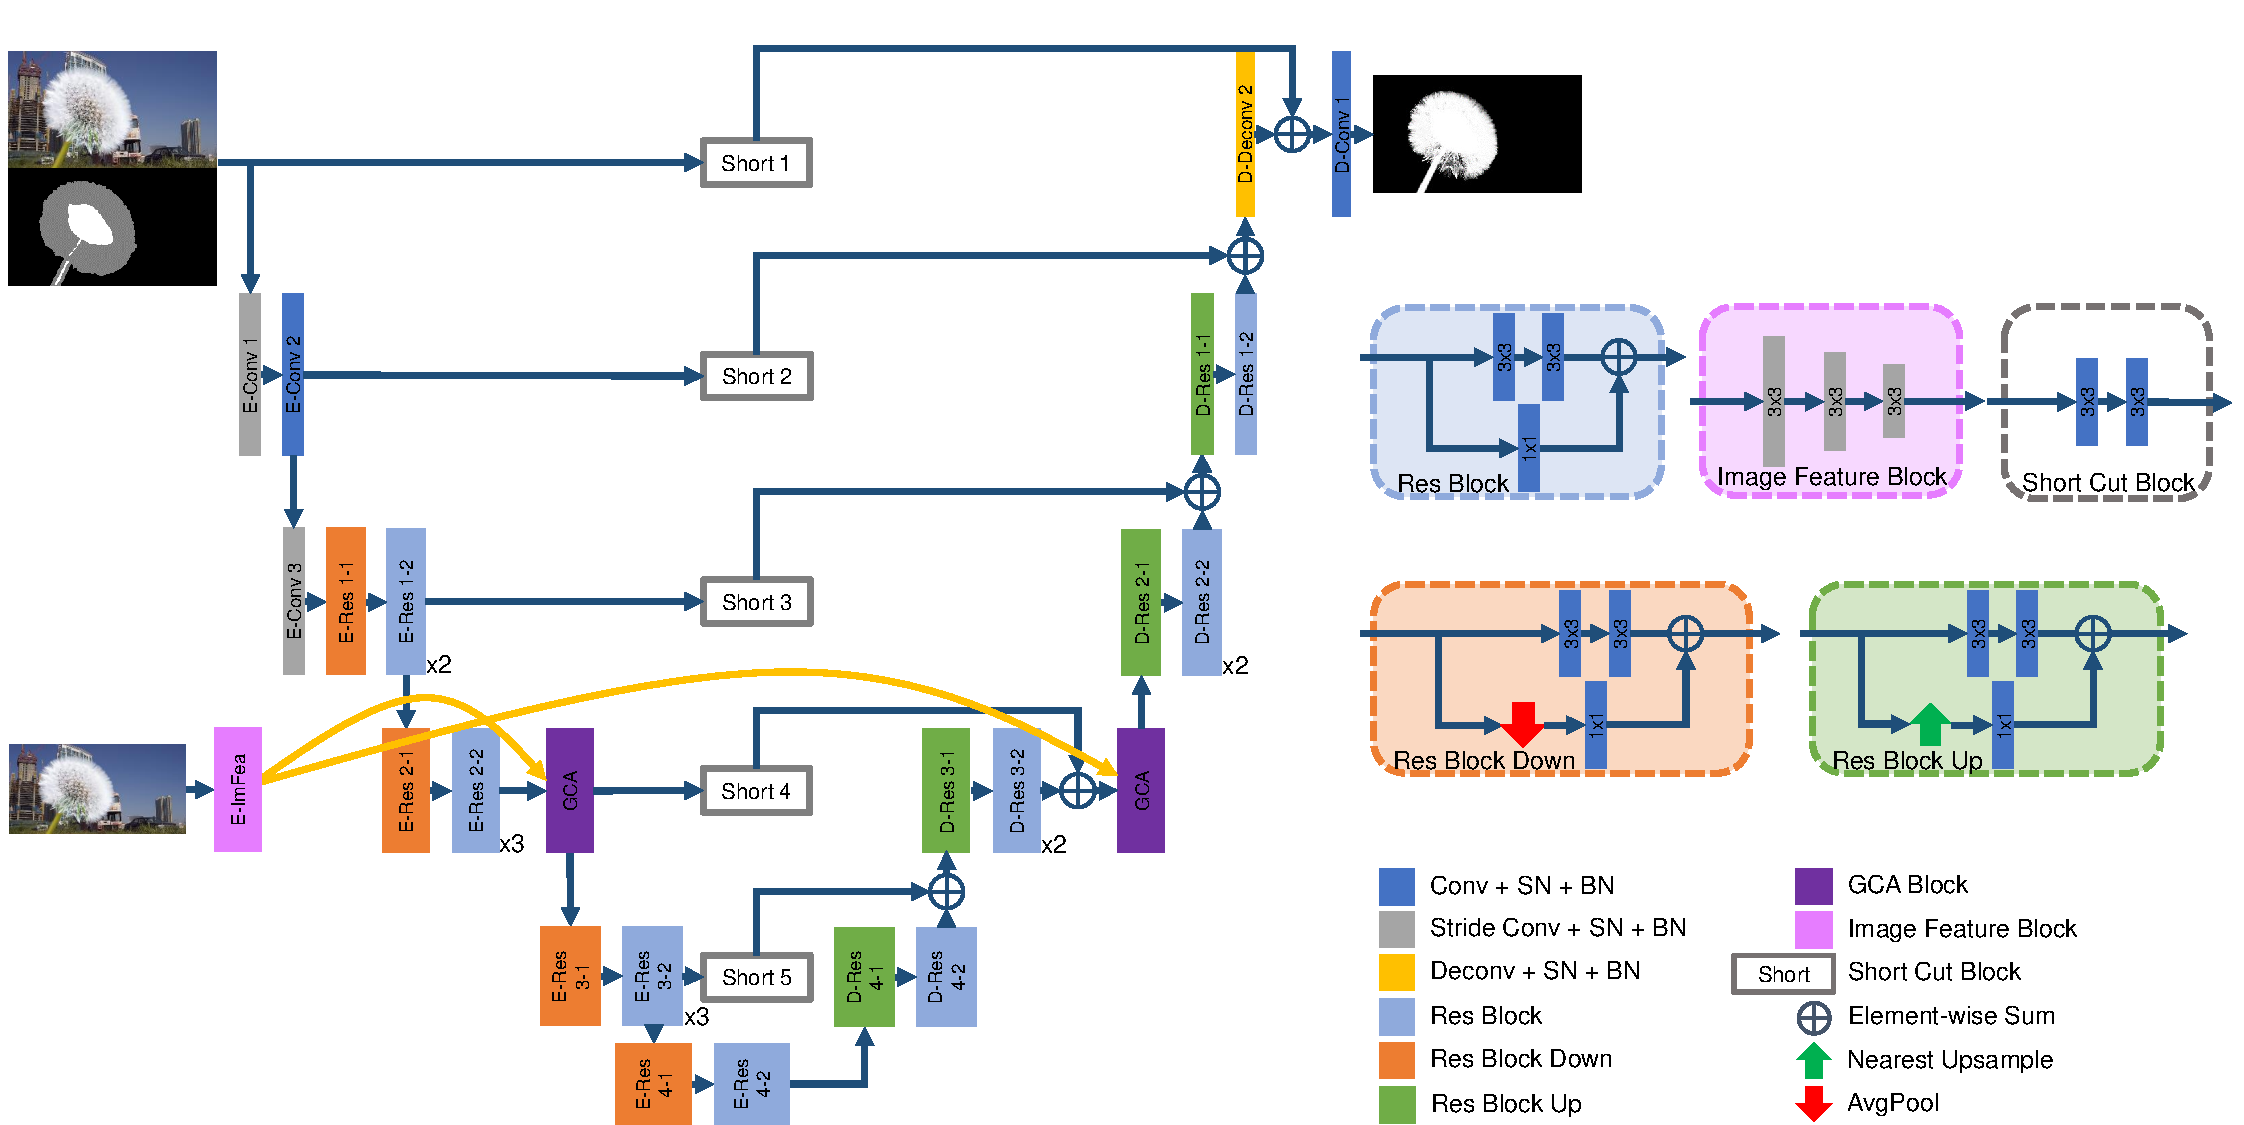
\includegraphics[width = 1\textwidth]{chap5/10261arch1.pdf}
	\bicaption{所提出的GCA Matting的网络结构细节图。基线网络模型具有相同的网络结构,但不具备图中的GCA机制部分以及图像特征模块。原始图像和trimap图像为alpha特征的输入数据,而图像特征模块仅将原始的合成图像作为输入数据。蓝色箭头表示alpha特征流,黄色箭头表示低级语义的图像特征流。GCA:引导上下文注意力;SN:谱归一化;BN:批归一化; $ \times N $:重复$ N $次}{Overview of our proposed guided contextual attention matting framework. The baseline model shares the same architecture without GCA mechanism and image feature block. Original image and trimap are the inputs of alpha feature. Image feature block only takes the original merged image as input. The blue arrows denote alpha feature flow and yellow arrows denote low-level image feature flow. GCA: guided contextual attention; SN: spectral normalization; BN: batch normalization; $ \times N $: replicate $ N $ times}
	\label{fig5:arch}
\end{figure}

\subsection{基线网络结构}
在近几年的图像抠图\cite{lutz2018alphagan,samplenet,lu2019indices}、图像分割\cite{long2015fully}、图像转换\cite{isola2017image}和图像补全\cite{liu2018image}任务中,类U-Net网络结构非常流行。在图\ref{fig5:arch}中给出了具有附带的GCA机制的基线网络结构。图中的网络结构与我们所设计的基线网络模型的唯一区别在于基线网络中没有GCA机制,因此也就没有其上游的图像特征模块(Image Feature Block)。

该基线网络的输入为裁剪后的图像块和3通道独热编码(one-hot encoding)的trimap图,它们被拼接为一个6通道输入。输出是相应的预测alpha遮罩值。
基线网络结构被设计为具有堆叠残差模块(stacked residual blocks)\cite{he2016deep}的编码器-解码器网络。

由于低级图像特征能对在alpha遮罩中保留纹理信息起到至关重要的作用,因此在我们自定义的基线模型中,解码器在上采样块之前(而不是在每个上采样块之后)对编码器输出的特征进行合并。这是因为预期中这些编码器特征具有更多的低级图像特征,而这样的设计可以避免在低级特征上进行更多的卷积计算。我们还使用了具有两层卷积层的跳层(short cut)块来对齐编码器特征的通道以进行特征融合。同时,与仅结合了不同的中级特征的典型U-Net结构不同,我们将原始输入直接通过跳层块传递到最后的卷积层。这些特征不与主干网络共享任何计算。因此,此跳层分支仅关注细节上的的纹理和梯度信息。

除了广泛使用的批归一化\cite{ioffe2015batch},我们还将谱归一化\cite{miyato2018spectral}引入每个卷积层,以对网络的Lipschitz常数添加约束达到稳定训练的效果,该设计方案普遍存在于图像生成任务中\cite{brock2018large,zhang2018self}。

\subsection{损失函数}
在所提出的神经网络的训练中,我们仅使用了一个alpha预测损失。alpha预测损失可以定义为每个像素的alpha预测值和标注的真实值之间的绝对差在整个未知区域上的平均值:
\begin{equation}
\mathcal{L} = \frac{1}{|\mathcal{U}|} \sum_{i\in \mathcal{U}}|\hat{\alpha_i}-\alpha_i|,
\label{eq5:loss}
\end{equation}
其中$ \mathcal {U} $表示在trimap中标记为未知区域的像素集合,$ \hat{\alpha_i} $和$ \alpha_i $分别表示像素位置$ i $的alpha遮罩预测值和真实值。

在先前的部分相关工作中,针对深度图像抠图任务,有一些新的损失函数被提出来,例如合成损失函数\cite{xu2017deep},梯度损失函数\cite{samplenet}和Gabor损失函数\cite{li2019inductive}。
Deep Matting\cite{xu2017deep}中使用的合成损失函数是通过计算由真实前景,背景和预测alpha遮罩所合成的预测图像与原始输入图像之间的绝对差作为损失。
梯度损失计算未知区域中alpha预测值梯度和真实值梯度之间的平均绝对差。
文献\parencite{li2019inductive}中提出的Gabor损失通过用一系列Gabor过滤器代替了梯度损失中的梯度算子,旨在能在纹理和梯度方面提供比梯度损失更全面的监督。

我们对这些损失进行了深入的研究,以揭示添加这些不同的损失是否可以使基线模型中的alpha值预测效果得到提升。我们在表\ref{tab5:ablation}中提供了在Composition-1k测试集\cite{xu2017deep}上进行的消融实验结果。如表\ref{tab5:ablation}所示,对预测结果的均方误差(Mean Square Error,MSE)和梯度误差(Gradient error,Grad)评测误差而言,引入合成损失函数不会带来任何显着差异,并且当我们将梯度损失加入到alpha预测损失时,给出的两种评测误差都会增加。尽管采用Gabor损失可以在一定程度上降低Grad梯度误差,但也会稍微提高MSE结果。因此,我们仅在模型中选择alpha预测损失作为唯一的损失函数。


\begin{table}[t]
	\bicaption{基线网络结构上的数据增广和不同损失函数的消融实验结果。定量实验结果测试于Composition-1k测试集。Aug:数据增广;Rec:alpha预测损失;Comp:合成损失;GradL:梯度损失;Gabor:Gabor损失}{Ablation study on data augmentation and different loss functions with baseline structure. The quantitative results are tested on Composition-1k testing set. Aug: data augmentation; Rec: alpha prediction loss; Comp: compositional loss; GradL: gradient loss; Gabor: Gabor loss.}
	\centering
	\setlength{\tabcolsep}{8pt}
	\begin{tabular}{ccccc|cc}  
		\toprule
		Aug&Rec&Comp&GradL&Gabor& MSE & Grad\\% & SAD &Conn
		\midrule
		\checkmark&\checkmark&&& & 0.0106 & 21.53 \\  % & {40.62}& 38.43
		\checkmark&\checkmark&\checkmark&&& 0.0107  & 21.85\\% & 40.85  & 38.73
		\checkmark&\checkmark&&\checkmark& & 0.0108 & 22.51\\ % & 43.62  & 42.19
		\checkmark&\checkmark&&&\checkmark & 0.0109 & 20.66\\ % & 42.53  & 40.84   
		&\checkmark&&& & 0.0146 & 32.01 \\%& 51.15& 51.52
		\bottomrule
	\end{tabular}
	\label{tab5:ablation}
\end{table}

\subsection{数据增广方法}
\label{sec5:aug}

由于文献\parencite{xu2017deep}中所提出的目前最主要的图像抠图数据集仅包含431个用于训练的前景对象,所以我们将数据增广视为基线模型的必须部分。
本节中我们将对一系列模型训练中使用的数据增广方案进行介绍。

首先,延续文献\parencite{samplenet}中的数据增广方案,我们以0.5的概率在前景图集合中随机选择两个前景物体图像,并将它们叠加组合以获得一个新的前景对象以及一个新的alpha图像作为采样数据。随后,以0.25的概率前景对象和alpha图像的大小将被调整为$640 \times 640 $,这样网络模型几乎可以看到整个前景图像,而不是裁剪后的局部图像块。然后,在前景图像和相应的alpha图像上进行随机的仿射变换。在此仿射变换中,我们定义了随机旋转,缩放,斜切以及垂直和水平翻转。再后,通过5到29中采样随机数作为像素数对alpha图像进行膨胀和腐蚀来生成trimap。获得trimap后,我们分别随机从每个前景图像中、alpha图和trimap图中的对应位置裁剪一个$ 512 \times 512 $的区块,所有裁剪的区块的中心像素都落在trimap图的未知区域上。然后将前景图像转换到HSV空间,并对色度,饱和度和明度分别施加不同的噪声。
最后,我们从MS COCO数据集\cite{lin2014microsoft}中为每个增广后的前景块随机选择一个背景图像,并将其合成为一张图像作为原始输入图像。

为了证明数据增广的有效性,我们进行了一个只包含最少数据增广的实验。在这种情况下,仅保留两个必要的操作,即图像裁剪和trimap图的膨胀生成。此实验中不包括更多的例如随机图像缩放和翻转这些在大多数先前的深度图像抠图方法\cite{xu2017deep,lutz2018alphagan,samplenet,lu2019indices}中被广泛使用的增广方式。我们将此实验设置视为无数据增广。实验结果被列在表\ref{tab5:ablation}中。我们可以看到,在不进行额外数据增广的情况下,我们的基线模型已经可以与Deep Matting方法的效果相媲美。

\section{引导上下文注意力抠图模型}
本节将对所提出的仅包含单层次引导上下文注意力机制的GCA Matting模型进行介绍。完整的引导上下文注意力机制包含两种组件,一个是用于低级图像特征抽取的图像特征提取器,另一个是用于信息传播的引导上下文注意力模块。

\begin{figure}[t]
	\centering
	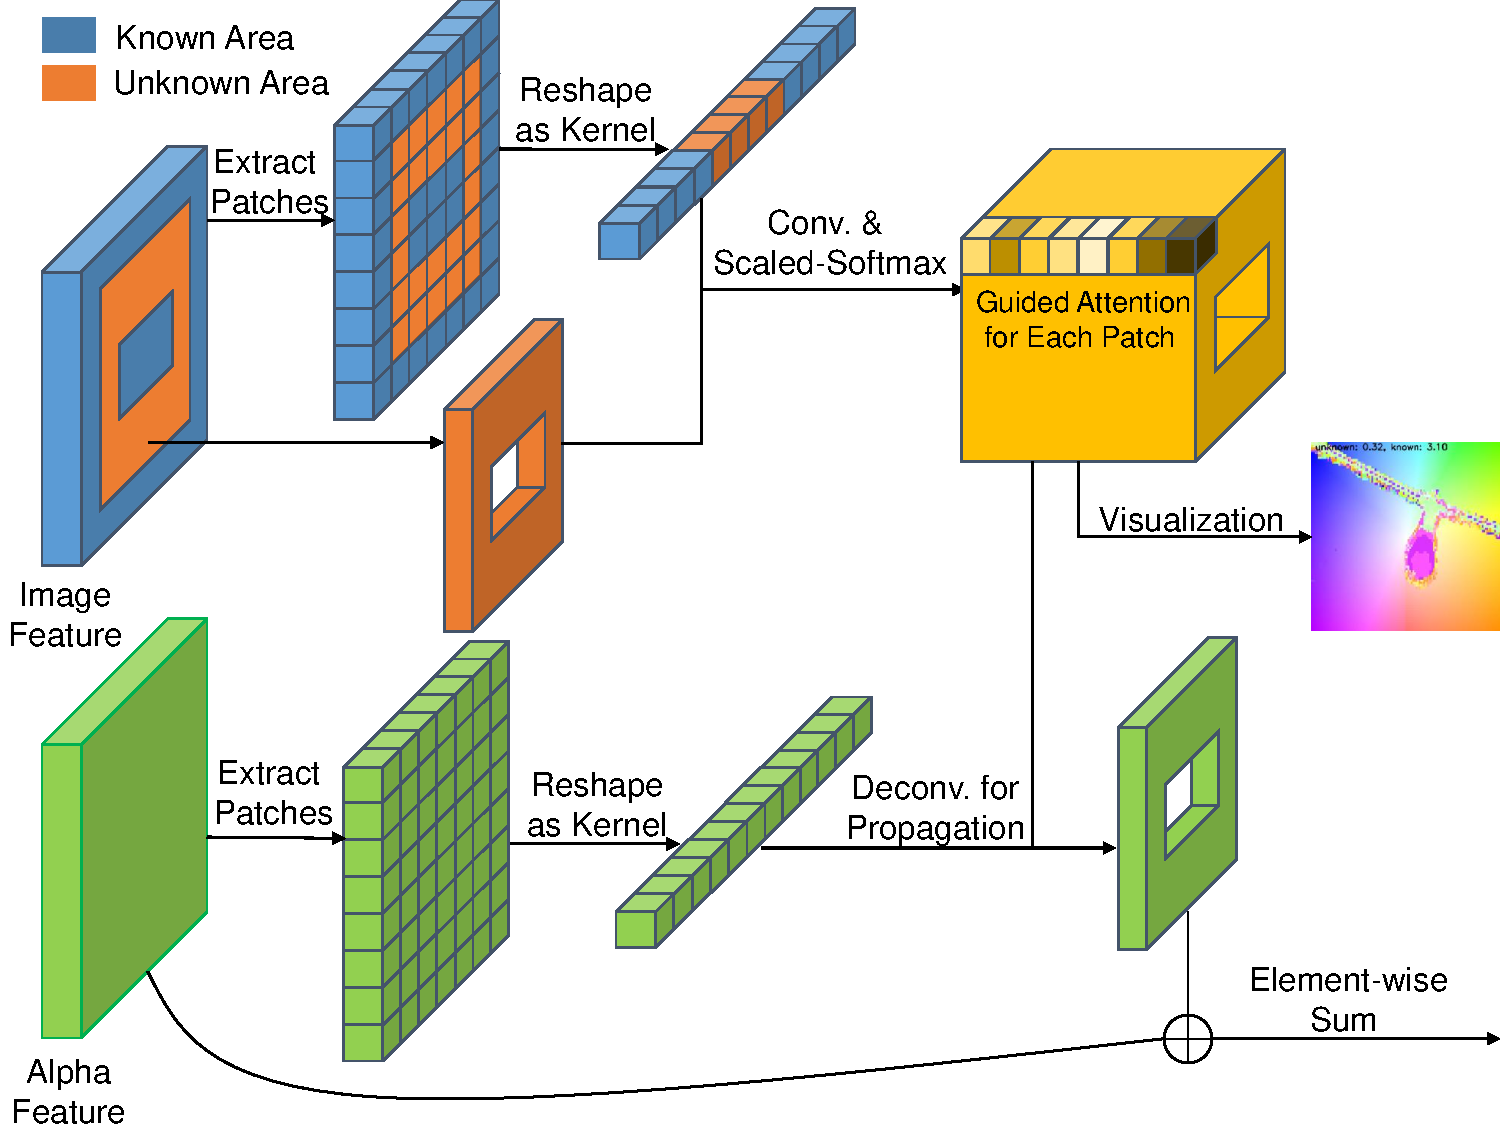
\includegraphics[width = 0.85\columnwidth]{chap5/10261block.pdf}
	\bicaption{引导上下文注意力模块图示。计算过程通过卷积或转置卷积进行实现。为了保持图示整洁,该图中未显示另外两个用于特征对齐的$1\times 1$的卷积层。一个在提取区块之前应用于输入的图像特征,另一个在逐元素求和之前应用于传播结果}{The illustration of the guided contextual attention block. Computation is implemented as a convolution or a deconvolution. Two additional $ 1\times 1 $ convolutional layers for adaptation are not shown in this figure to keep neat. One is applied to the input image feature before extracting patches, and the other one is applied to the result of propagation before the element-wise summation}
	\label{fig5:gca}
\end{figure}

\subsection{低级图像特征}

大多数基于相似性的方法都具有一个基本的归纳偏置,即外观几乎相同的局部区块应具有相似的不透明度。该归纳偏置允许基于相似性的抠图算法将alpha值从trimap图中的已知区域传播到未知区域,这通常可以产生非常出色的alpha预测效果。

因此,我们在所提出的框架中定义了两个不同的特征流(图\ref{fig5:arch}):alpha特征流(蓝色箭头)和图像特征流(黄色箭头)。其中alpha特征是从由原始图像和trimap图拼接产生的6通道输入生成的。最终的alpha遮罩值可以直接从该特征中预测,故称为alpha特征。低级图像特性与高级alpha特征形成对比,这些特征仅由具有步长(stride)为2的三个卷积层序列从输入图像生成,这类似于传统的基于相似性的方法中所用到的的局部颜色统计量。

具体来说,alpha特征包含不透明度信息,而低级图像特征包含外观信息。
在提供不透明度和外观信息的情况下,GCA机制可以学习到一个前几章中所多次用到的相似性图,并通过类似于基于相似性的抠图方法进行不透明度传播。
换句话说,我们利用低级图像特征来指导alpha特征上的信息流动。

\subsection{引导上下文注意力模块}
受文献\parencite{yu2018generative}中上下文注意力模块的启发,我们在抠图问题中引入了引导上下文注意力模块。

如图\ref{fig5:gca}所示,引导上下文注意力同时利用了图像特征和alpha特征。首先图像特征被分为已知部分和未知部分,并从全部的图像特征中抽取$3\times 3$的区块。每个特征块表示一个特定未知的外观信息。我们将特征块变形为卷积核。为了能够对一个中心$ (x,y)$在未知区域的图像特征块$ U_{x,y} $和一个中心在$ (x',y') $的图像特征块$ I_{x', y'} $之间的相关性进行度量,相似性被定义为归一化的内积形式:
\begin{equation}
	s_{(x,y), (x',y')} = 	
	\begin{cases}
	\lambda \quad &(x,y)=(x',y');\\
	\langle \frac{U_{x, y}}{\|U_{x, y}\|},\frac{I_{x', y'}}{\|I_{x', y'}\|}\rangle \quad &\mathrm{otherwise},	
	\end{cases}
\end{equation}
其中$ U_{x, y}\in\mathcal{U}$也是图像特征块集合 $ \mathcal{I} $中的一个元素,即$ \mathcal{U} \subseteq \mathcal{I} $。常数$ \lambda $ 为惩罚参数,可以避免未知区域的特征块和自身之间产生很大的相关性,在模型中我们采用$ \lambda =-10^4$。在实现中,该相关性可以通过未知区域特征块与图像特征块经由变形生成的卷积核进行卷积计算得到。给定一个相关性,则可以在$ (x',y') $维度上进行归一化指数函数(softmax)计算,得到每个特征区块上的引导注意力值:
\begin{equation}
	a_{(x,y), (x',y')} = \mathrm{softmax}(w(\mathcal{U}, \mathcal{K}, x',y')s_{(x,y), (x',y')}),
\end{equation}
\begin{equation}
w(\mathcal{U}, \mathcal{K}, x',y') = \begin{cases}
\mathrm{clamp}(\sqrt{\frac{|\mathcal{U}|}{|\mathcal{K}|}}) \quad I_{x',y'} \in \mathcal{U};\\
\mathrm{clamp}(\sqrt{\frac{|\mathcal{K}|}{|\mathcal{U}|}}) \quad I_{x',y'} \in \mathcal{K},
\end{cases}
\label{eq5:weight}
\end{equation}
\begin{equation}
\mathrm{clamp}(\phi) = \mathrm{min}(\mathrm{max}(\phi, 0.1), 10),
\end{equation}
其中$ w(\cdot)$是权重函数,$ \mathcal{K} = \mathcal{I}-\mathcal{U} $是来自已知区域的图像特征块集合。与图像补全任务不同的是,trimap图中未知区域的面积不受任何控制。在许多输入的trimap图中,存在极大的未知区域而几乎没有已知的像素。因此,仅将不透明度信息从已知区域传播到未知部分通常是不可行的。在所提出的引导上下文注意力机制中,我们让未知部分同时借用已知区域和未知区域中的特征。根据每个区域的面积,通过公式(\ref{eq5:weight})中所定义的权重函数,将不同的权重分配给已知和未知的区域。如果已知区域的面积较大,则已知区域的特征块可以传达更准确的外观信息,从而暴露出前景和背景之间的差异,因此,我们将给已知区域特征块分配较大的权重。而如果未知区域的面积很大,则已知区域的图像特征块只会提供一些局部的外观信息,这可能会损害到不透明度的传播,所以,我们将较小的权重分配给已知区域特征块。

当从图像特征得到引导注意力值后,可以根据由引导注意力值所定义的相似性矩阵,在alpha特征上进行信息传播。
与图像特征类似,从alpha特征中提取特征块并将其变形为卷积核。信息传播过程可以通过引导注意力值与变形后的alpha特征块之间的转置卷积计算完成。该转置卷积可在未知区域中重建alpha特征,并对转置卷积中相互覆盖的像素值取平均。最后,我们通过逐元素求和对输入的alpha特征和传播结果进行融合。这种逐元素求和作为一个残差连接可以对模型训练起到稳定作用。

在此方法所隐含的相似性图中,每个节点都有两种不同的特征,即不透明度alpha特征和图像外观特征。图像外观特征仅用于生成相似性图中的边缘权重,而不透明度alpha特征是实际上的待传播信息。从图\ref{fig5:gca_comp}可以从图的角度看出所提出的GCA模块与上下文注意力机制及自注意力机制之间的区别。GCA机制中每个点对应于两个不同空间的特征,一个用于引导,一个用于承载信息。可以看出在不同的特征空间上数据点之间的相似性是不相同的,这可以类比于前文多模态约束传播中不同模态上的相似性矩阵的不同。

\begin{figure}[t]
	\centering
	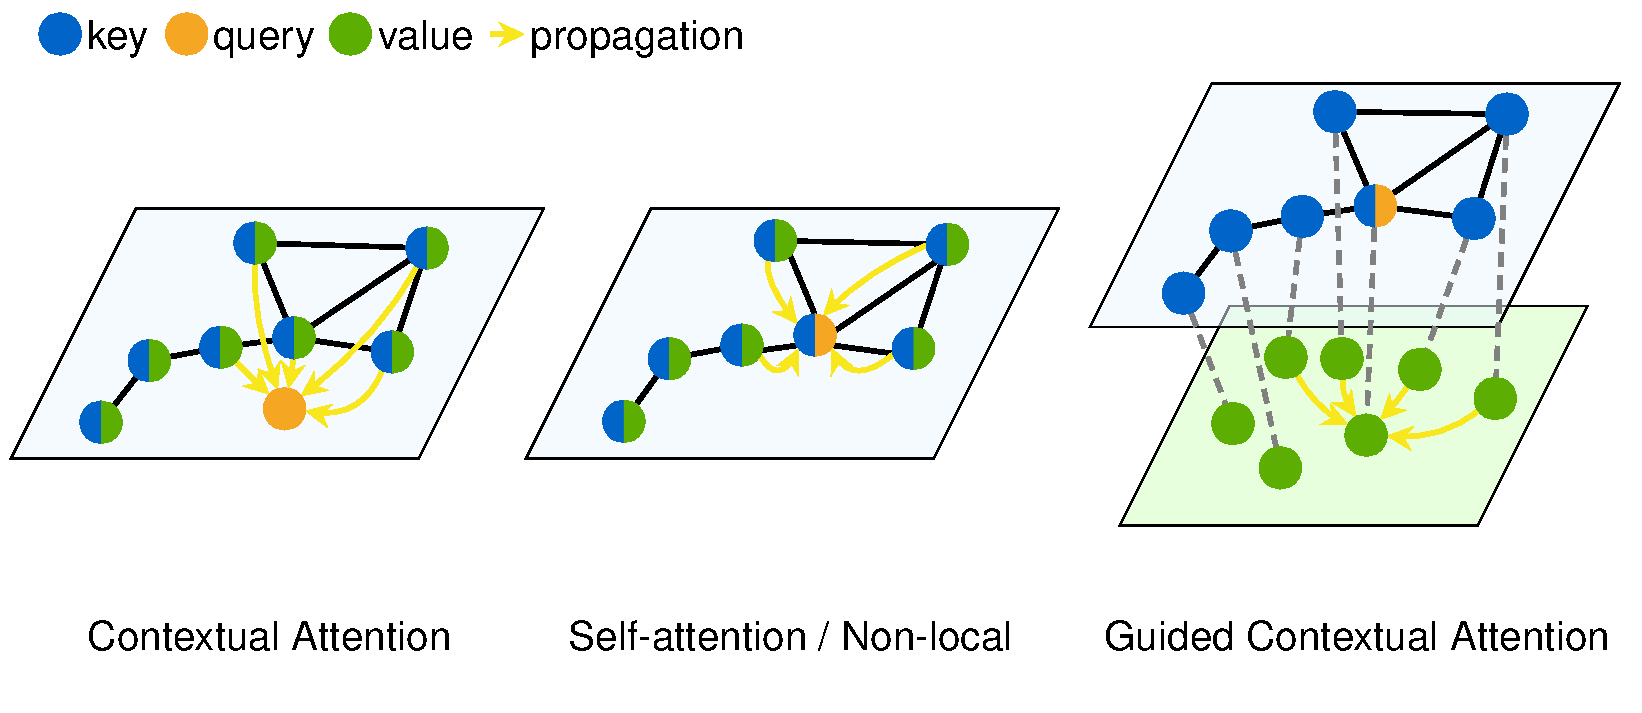
\includegraphics[width = 0.85\columnwidth]{chap5/GCA-compare.pdf}
	\bicaption{在相似性图角度下上下文注意力、自注意力/Non-local和引导上下文注意力的对比。每个平面代表一种特征空间}{Comparison between Contextual Attention, Self-Attention/Non-local and Guided Contextual Attention through the lens of affinity graph. Each plain indicate a feature space }
	\label{fig5:gca_comp}
\end{figure}

\subsection{神经网络实现细节}
多数基于相似性的经典抠图方法最终产生一个依赖于图拉普拉斯的闭式解\cite{levin2008closed,lee2011nonlocal,chen2013knn}。闭式解可以被看作是信息传播算子的不动点,或者是传播迭代趋于无穷时收敛到的极限值\cite{zhou2004learning}。
在基于相似性抠图的经典算法中,图拉普拉斯矩阵大多通过手工设计的固定计算方式生成,而不依赖于数据本身的分布特性。在本章所提出的两个抠图模型中,所使用到的相似性矩阵皆是通过神经网络特征计算得出,然而,神经网络参数本身是通过训练数据学习而来。所以,本章所提出的抠图方法本质上是通过数据驱动,在训练集上学习相似性矩阵的生成方式,以此提升纯端到端的深度抠图网络的性能。同时,不同的图像外观特征分支也会生成不同的相似性矩阵。因此,我们在主干网络中对称地将两个引导上下文注意力模块插入到同一层次的编码器和解码器上。该设计目的在于使数据在模型中进行更多次的传播,并充分利用不透明度的信息流。

当在更高分辨率特征上计算引导上下文注意力时,模型就可以关注到更细节的外观信息。但是,另一方面,注意力模块的计算复杂度为$ O(c(hw)^2)$,其中$ c、h、w $分别是特征图的通道、高度和宽度。因此,我们将两个引导注意力模块添加到尺寸层次为$ 64 \times 64 $的网络阶段中。

在Adobe Image Matting数据集\cite{xu2017deep}上,我们对GCA Matting的网络进行了$ 200,000 $次迭代训练,批大小(batch size)为40。训练中使用了$ \beta_1 = 0.5 $和$ \beta_2 = 0.999 $的Adam优化器\cite{kingma2014adam}执行优化。学习率初始化为$ 4 \times 10^{-4} $,在学习率上使用了预热(warmup)和余弦衰减(cosine decay)\cite{loshchilov2016sgdr,goyal2017accurate,he2019bag}策略。

\section{层次化不透明度传播抠图模型}
在上一节所提出的GCA Matting模型的基础上,为了在高分辨率级别的特征上对整个输入图像实现直接的不透明度信息传播,本节提出了新的层次化不透明度传播(Hierarchical Opacity Propagation,HOP)结构,其中所提出的神经网络结构可以看作是每层具有不同的图连接权重的多层图卷积网络\cite{kipf2016semi},且不透明度可以在任意两个像素之间实现传播。
在本节中,我们将首先介绍层次化不透明度传播的基本模块,即HOP模块,然后针对HOP模块提出尺度不敏感位置编码(scale-insensitive positional encoding),最后对模型实施细节进行描述。

\begin{figure}[t]
	\centering	 
	\subfloat[]{
		\centering
		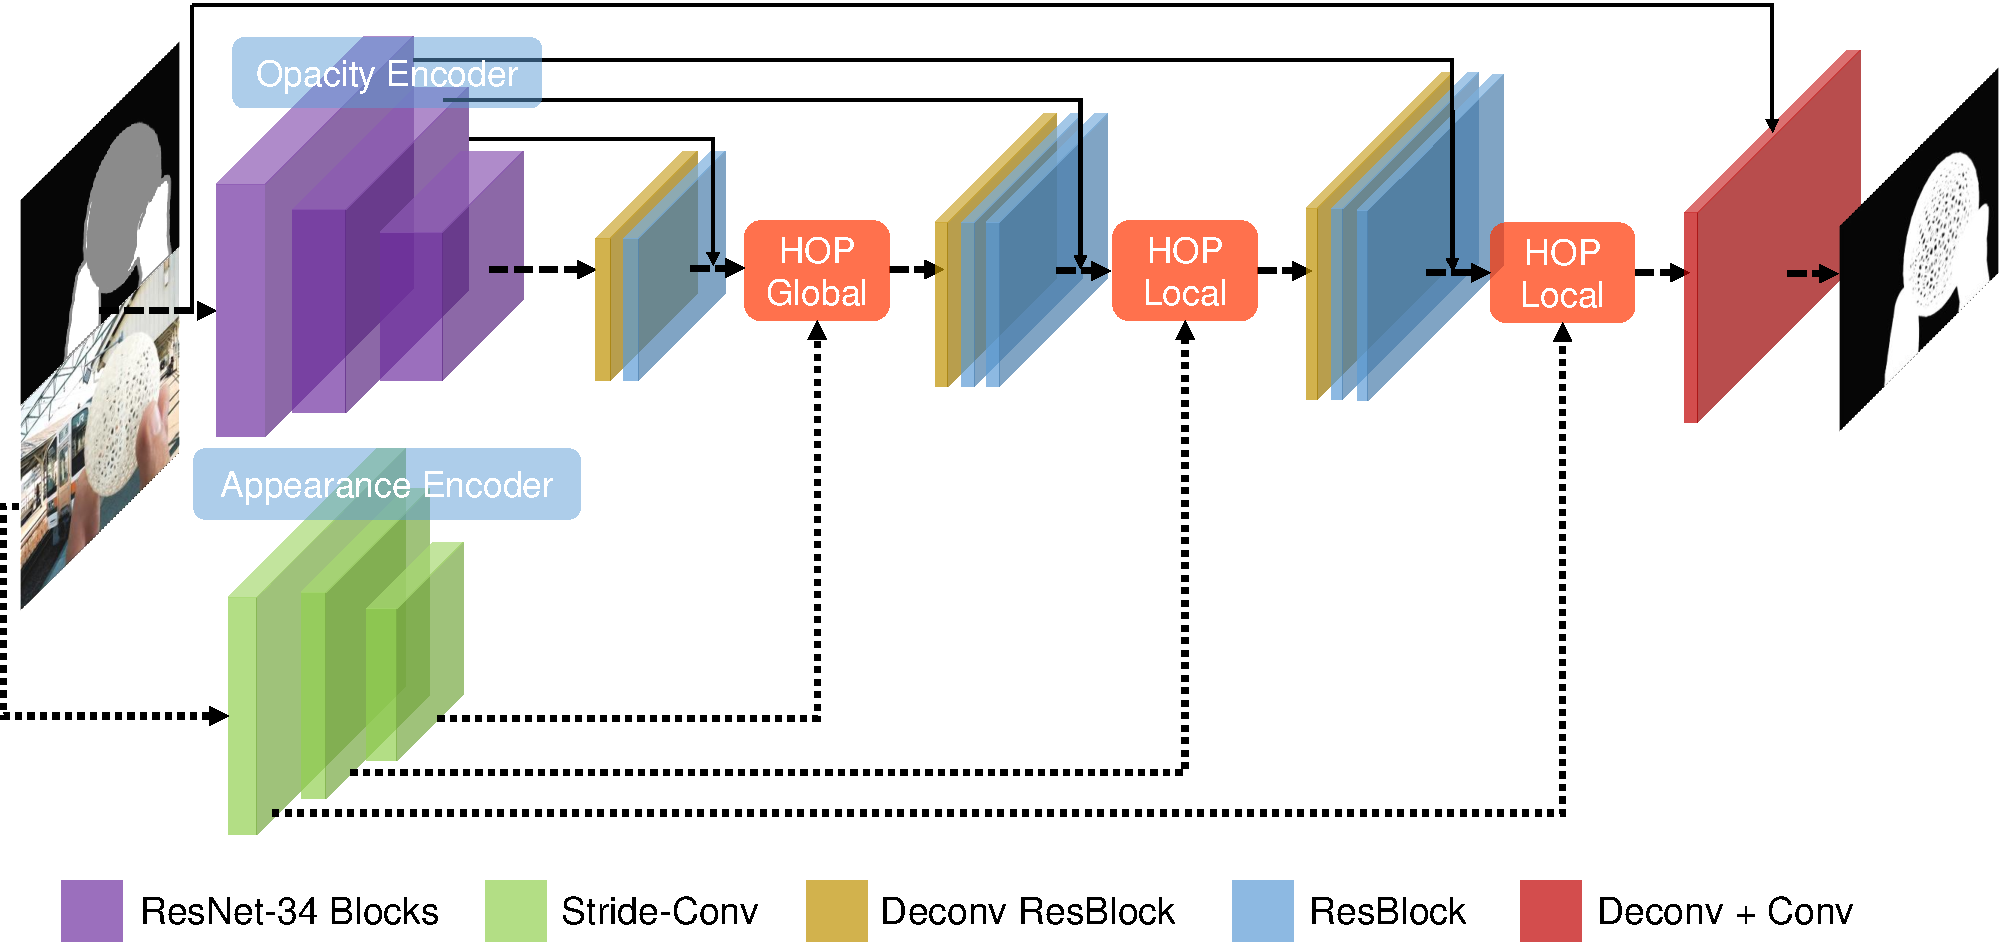
\includegraphics[width=0.66\linewidth]{chap5/arch.pdf}
		\label{fig5:diaga}
	}
	\centering	 
	\subfloat[]{
		\centering
		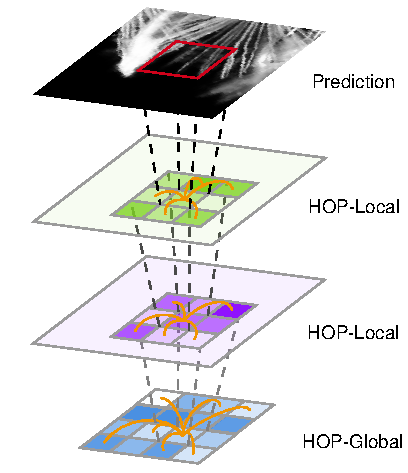
\includegraphics[width=0.33\linewidth]{chap5/diagram.pdf}
		\label{fig5:diagb}
	}
	\bicaption{所提出的HOP结构示意图。为了便于表示,图中仅示出了具有4个尺度等级的解码器和2个局部HOP模块。在具体实现中,网络模型具有包含5个尺度等级解码器和3个局部HOP块。(a)所提出的网络架构,外观编码器分支仅将RGB图像作为输入;(b)在不同语义级别的特征图上层次化不透明度传播的示意图,橙色线表示特征的传播}{Diagrams of our proposed HOP structure. For the ease of representation, only a 4-scale-level decoder and 2 local HOP blocks are shown. In our implementation, we have a 5-level decoder and 3 local HOP blocks. (a) The architecture of our network. The appearance encoder branch only takes RGB image as the input. (b) The schematic diagram of hierarchical opacity propagation on feature maps from different semantic level. Orange lines indicate the feature propagation}
	\label{fig5:diag}
\end{figure}

\subsection{层次化不透明度传播模块}
通常情况下,Non-local模块\cite{wang2018non}或Transformer\cite{vaswani2017attention}能够通过其中的自注意力机制(self-attention mechanism)\cite{lin2017structured}进行全局信息传播。但是,如果直接在自然图像抠像方法中采用原始的Non-local模块或图像Transformer,则会存在两个严重的缺陷。一方面,Non-local模块在计算代价很高,因此GCA Matting仅在特征尺寸较小的部分使用了与其相似的GCA机制。尽管为了减少计算量和内存消耗,有一些改进方法被提出\cite{zhu2019asymmetric},但对图像抠图这种需要在大尺寸特征图上进行不透明度信息传播的问题而言,依然不可行。另一方面,Non-local模块和Transformer都在唯一的输入特征图上构建一个完全图,并且完全图中边的权重是由节点的特征生成。在图像抠图任务中,每个节点的特征是不透明度信息。在某些语义任务(例如视频分类\cite{wang2018non},语义分割\cite{zhu2019asymmetric}或图像补全\cite{yu2018generative})中,基于不同特征节点之间的相似性传播语义特征相对而言非常直观且可行,而在自然图像抠图任务中传播过程需要更多的无语义的外观信息,而不是语义信息。


\begin{figure}[t]
	\centering
	\bisubcaptionbox{局部HOP模块\label{fig5:blocka}}%
					{local HOP block}
					[0.24\textwidth]{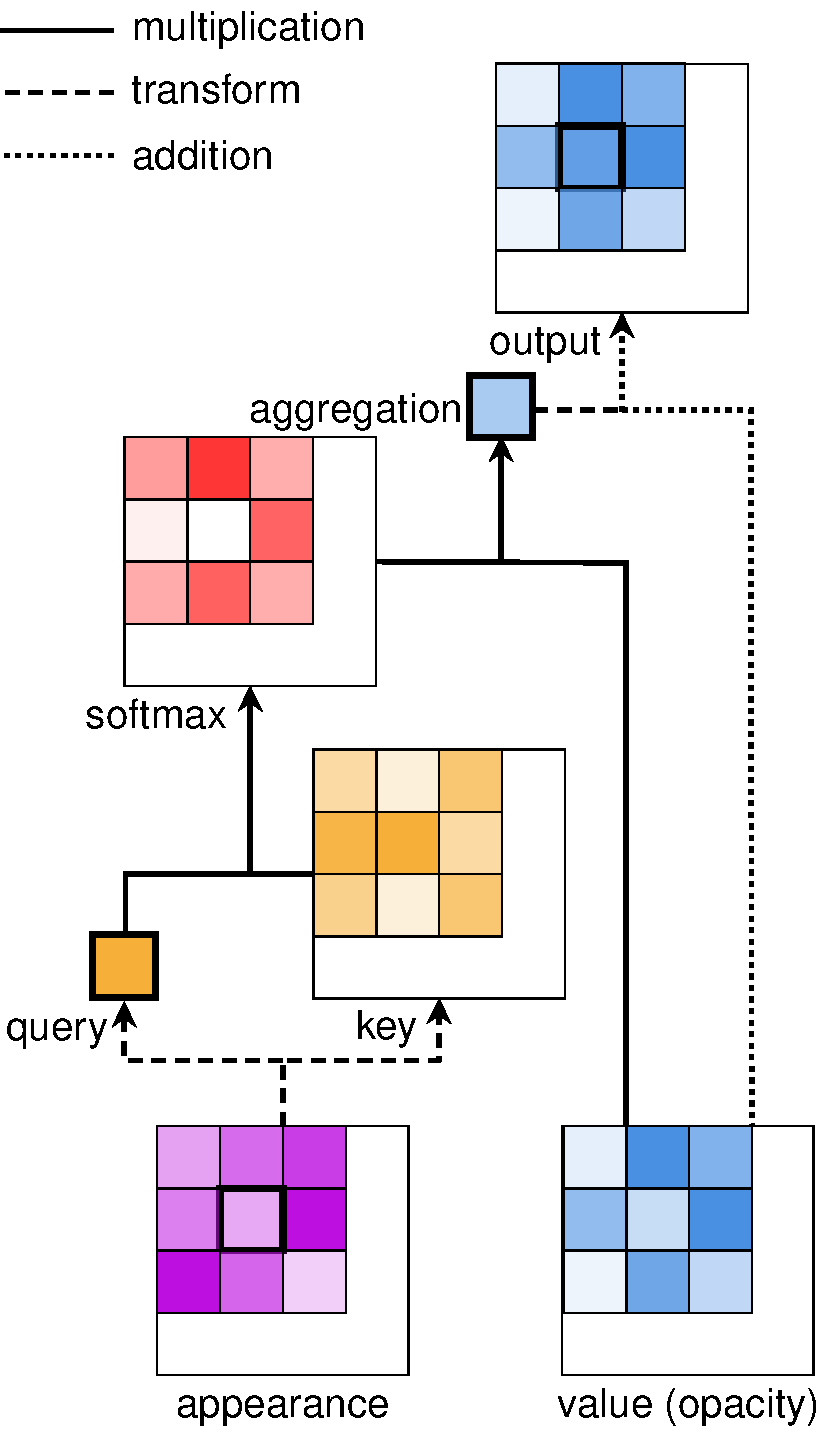
\includegraphics[height=.35\textwidth]{chap5/HOP-local.pdf}}
	\bisubcaptionbox{局部自注意力\label{fig5:blockb}}%
					{local self-attention}
                    [0.24\textwidth]{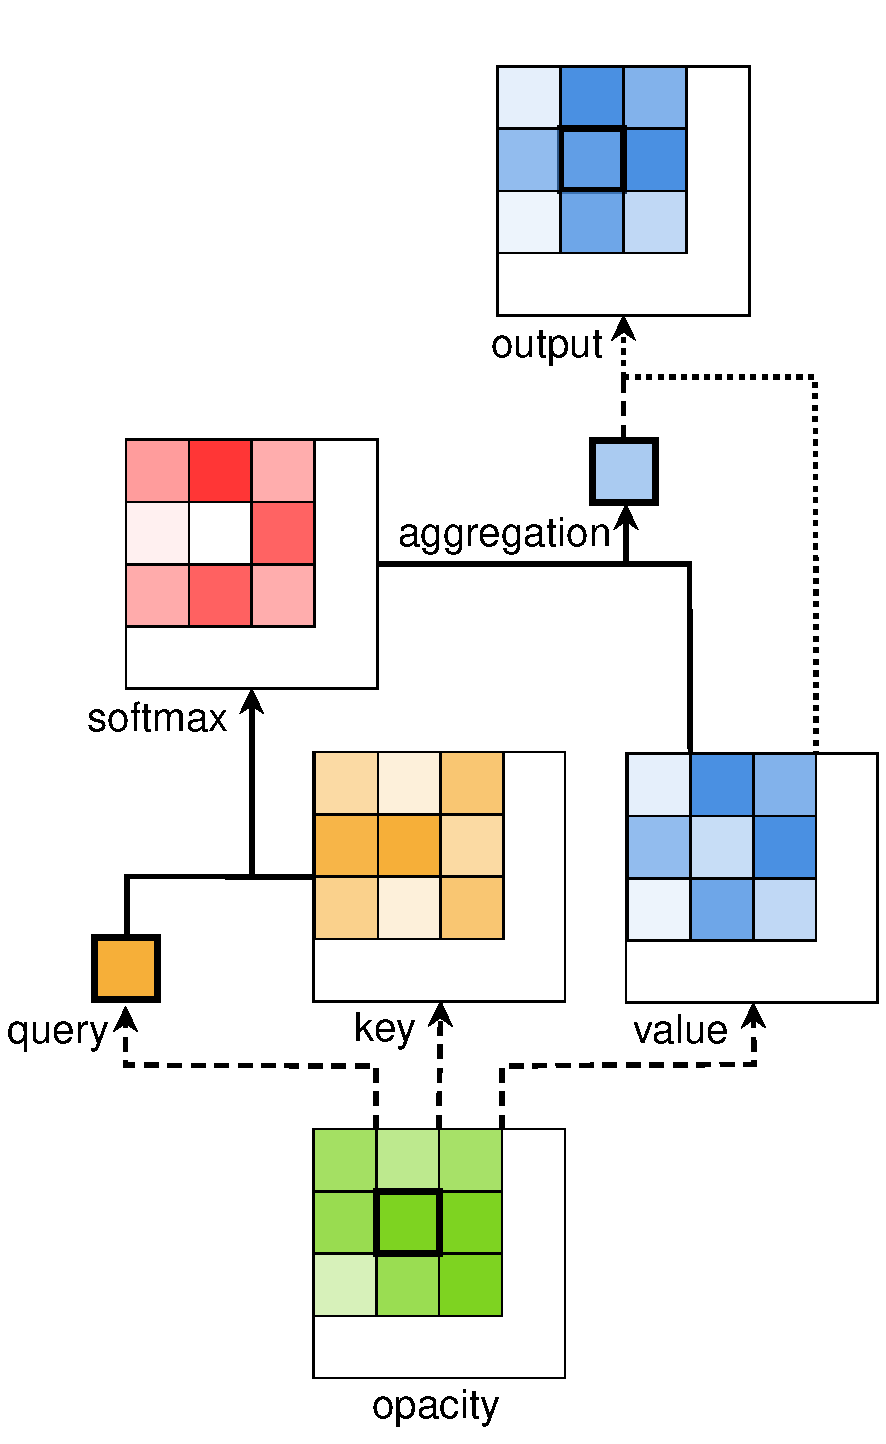
\includegraphics[height=.35\textwidth]{chap5/SA-local.pdf}}                  
	\centering
	\bisubcaptionbox{全局HOP模块\label{fig5:blockc}}%
					{global HOP block}
					[0.24\textwidth]{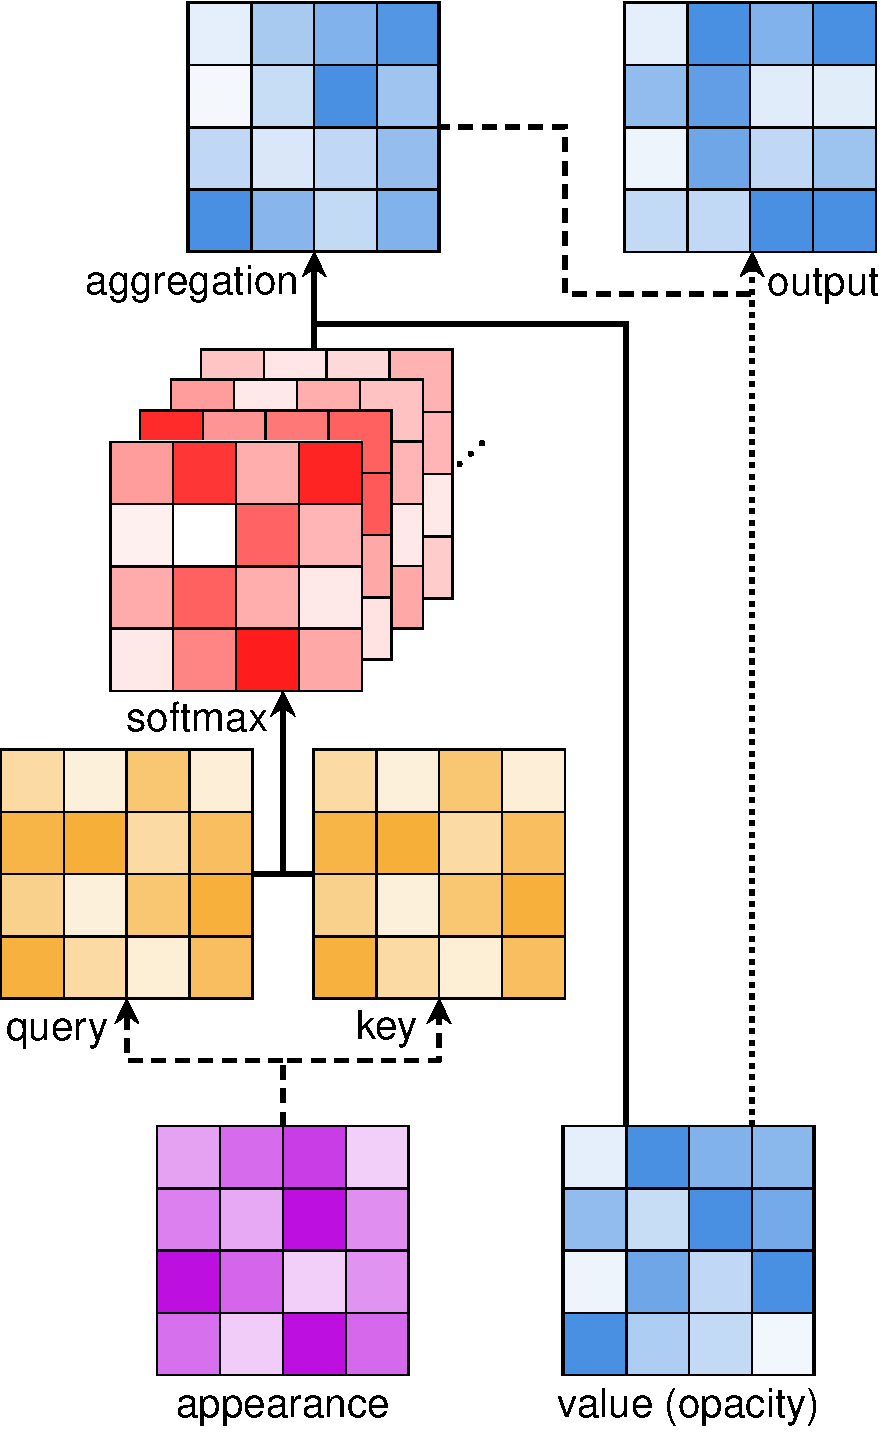
\includegraphics[height=.35\textwidth]{chap5/HOP-global.pdf}}
	\bisubcaptionbox{全局自注意力\label{fig5:blockd}}%
					{global self-attention}
					[0.24\textwidth]{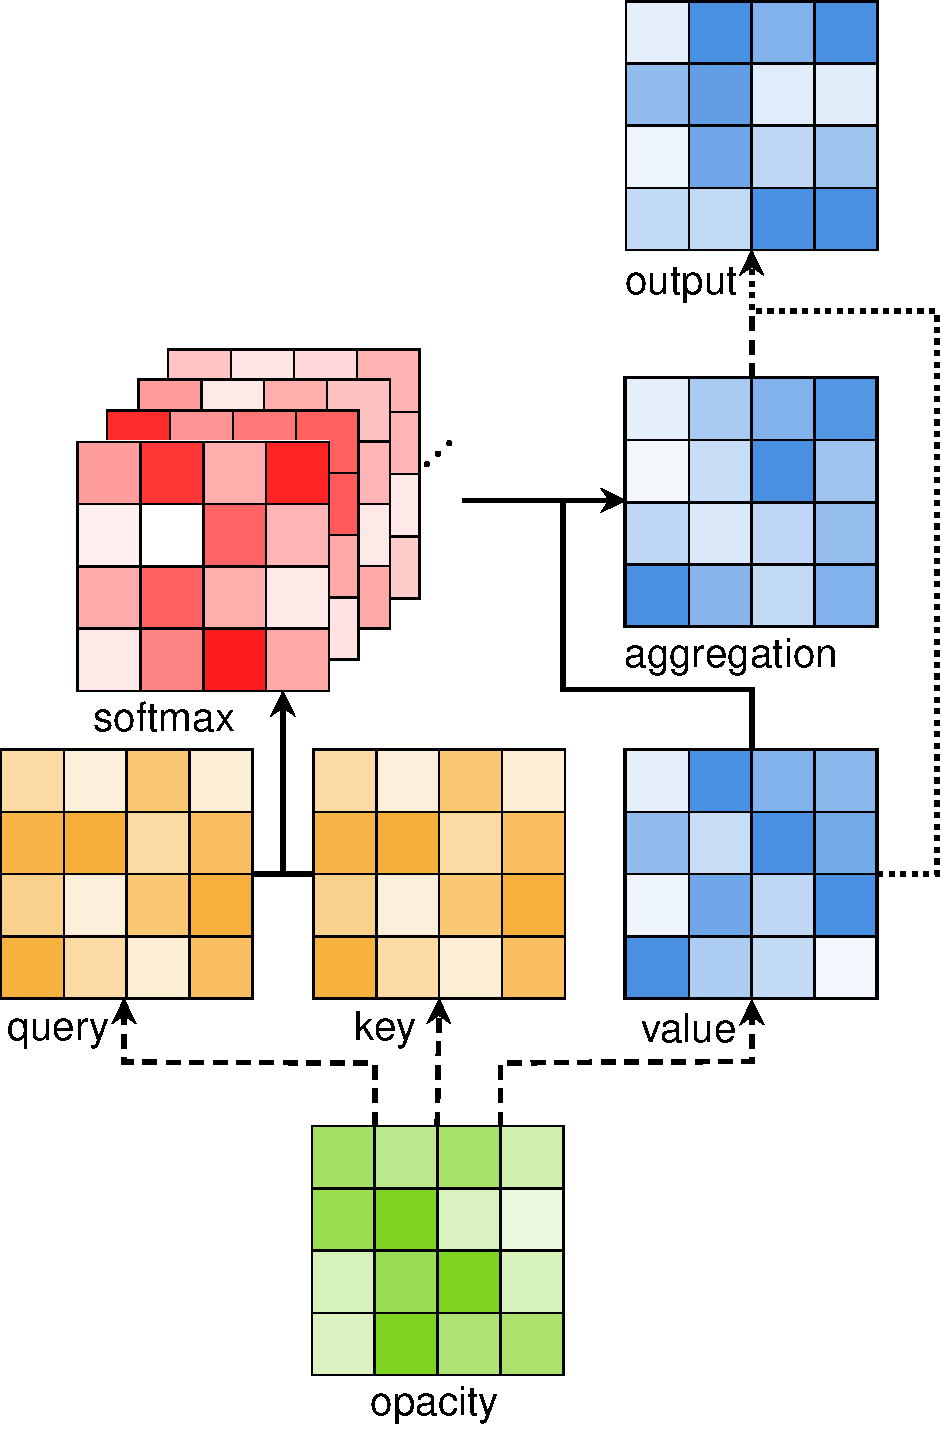
\includegraphics[height=.35\textwidth]{chap5/SA-global.pdf}}
	\bicaption{局部HOP模块、局部自注意力、全局HOP模块和全局自注意力的细节结构示意图,在两个局部模块示意图上为便于表示,仅展示了一个查询数据点}{The diagrams of detailed structure of local HOP block, local self-attention block, global HOP block and global self-attention block. For these two local blocks, we only show one query data point in the diagrams for the ease of presentation}
	\label{fig5:block}
\end{figure}

受到近期稀疏Transformer\cite{child2019generating,huang2019interlaced}和局部自注意力\cite{ramachandran2019stand}的成功的启发,在GCA Matting模型基础上,本节所提出的层次化不透明度传播结构包含了两种不同的传播模块,即全局HOP模块和局部HOP模块,两种模块在传播中同时利用了图像外观信息和不透明度预测信息。

所提出的HOP Matting的网络总体结构如图\ref{fig5:diaga}中所示。在该方法中,延续了GCA Matting模型的设计,具有两个编码器分支,一个作为不透明信息来源(即alpha遮罩信息),另一个作为图像外观信息来源。而全局HOP模块采用了GCA模块相同的构造形式,为便于下文中局部HOP模块的理解,在本节中,我们采用与注意力机制相似的数学形式重新对其进行定义。假设源自不透明度编码器和外观编码器的特征图分别被表示为$F^O\in\mathbb{R}^{HW\times C}$ 和$F^A\in\mathbb{R}^{HW\times C}$,特征图上位于 $(i,j)$的特征点为$f^O_{(i,j)}\in\mathbb{R}^{C}$和$f^A_{(i,j)}\in\mathbb{R}^{C}$,则全局HOP模块可定义为:
\begin{equation}
\begin{aligned}
q_{(i,j)} =& W_{QK}f^A_{(i,j)},\\ 
k_{(x,y)} =& W_{QK}f^A_{(x,y)}, \\
a_{(i,j),(x,y)} =& \mathop{\mathrm{softmax}}_{(x,y)}(\frac{q_{(i,j)}^Tk_{(x,y)}}{\|q_{(i,j)}\|\|k_{(x,y)}\|}),\\
g_{(i,j)} =& W_{out}(\sum_{(x,y)}a_{(i,j),(x,y)}f^O_{(x,y)}) + f^O_{(i,j)},
\end{aligned}
\end{equation}
其中$W_{QK}$为作用在键(key)与查询(query)上的线性变换,$W_{out}$ 是用于将传播后的信息与输入特征图$F^O$对齐的变换。此外,$F^O$在此处是不进行任何变换的注意力机制中的值(value)项,同时也可以将$v_{(x,y)}=W_{out}f^O_{(x,y)}$作为值项。图\ref{fig5:blockc}展示了全局HOP模块的结构细节。

不同于自注意力\cite{lin2017structured,vaswani2017attention}或者传统注意力机制\cite{bahdanau2014neural,xu2015show},在全局HOP模块中键和值是异源生成的。在自注意力机制中,查询、键和值都是从同一个特征中生成的,而在传统注意力机制中键和值也具有相同的信息来源。但是在HOP模块中,采用了GCA模块的思路,查询和键具有相同图像外观特征作为信息来源,而值项则以不透明度特征作为信息来源。

类似地,我们可以对只关注每个特征点的局部邻域的局部HOP模块进行公式化:
\begin{equation}
\begin{aligned}
a_{(i,j),(x,y)} = &\mathop{\mathrm{softmax}}_{(x,y)\in\mathcal{N}((i,j), s)}(\frac{q_{(i,j)}^Tk_{(x,y)}}{\|q_{(i,j)}\|\|k_{(x,y)}\|}),\\
g_{(i,j)} = &W_{out}(\sum_{(x,y)\in\mathcal{N}((i,j), s)}a_{(i,j),(x,y)}f^O_{(x,y)})\\& + f^O_{(i,j)},
\end{aligned}
\end{equation}
其中,$\mathcal{N}((i,j), s)$表示位于$(i,j)$特征点的窗口大小为$s$的空间近邻特征点集合。两种HOP模块与自注意力的区别可以从图\ref{fig5:gca_comp}或图\ref{fig5:block}中看出,在消融研究中,我们将所提出的两种HOP模块与全局/局部自注意力模块进行了性能对比。

利用前文所述的两种HOP模块,如图\ref{fig5:diagb}所示,我们构建了用于alpha遮罩值估计的完整的层次化不透明度传播(HOP)结构。一个HOP结构包括一个全局HOP模块和多个局部HOP模块。在示意图\ref{fig5:diagb}中,我们省略了HOP模块之间的卷积与反卷积层,以更清晰地显示如何层次化传播不透明度信息。底部的全局HOP模块将从神经网络的瓶颈处的特征图上进行全局的不透明度传播,该层次的特征图包含更多的语义信息但只有较少的纹理消息。
通过进行全局地语义特征传播以利用整个图像上全部的信息是一个非常直观的操作。随后,将局部HOP模块加入到网络中不同的反卷积阶段之间,在这些高分辨率特征图中存在更多的纹理表示信息。因此,这也促使了局部HOP模块仅需要关注每个查询点的空间局部近邻,以提取纹理信息。借助HOP结构,不透明度alpha特征可以在不同的特征级别上进行信息传播,先在语义特征上传播再到在纹理特征上传播,先在低分辨率特征图传播再到在高分辨率特征图上传播。

此外,所提出的HOP结构可以被视为一个4层的图卷积网络\cite{kipf2016semi},每层具有权重值不同的图结构,并且由于特征图的尺寸在变化,所以节点的数量在网络的不同阶段也是可变的。全局HOP模块中的图为完全图,而局部HOP模块中的相似性图是稀疏的。所有边权重均通过注意力机制进行计算,类似于图注意力网络(Graph Attention Networks,GATs)\cite{velivckovic2017graph}。

\subsection{位置编码}
在先前的一些工作中,自注意力机制中的位置编码总能带来一定的收益\cite{vaswani2017attention,dai2019transformer,ramachandran2019stand}。在本节中我们将对所提出的方法中加入的位置编码进行描述。我们采用两种不同的位置编码方式:全局HOP模块的尺度不敏感位置编码(scale-insensitive positional encoding)和局部HOP块的局部相对位置编码(local relative position encoding)。图\ref{fig5:PE}对不同的位置编码方法进行了展示。

\begin{figure}[t]
	% \subfloat{
	% 	\centering
	% 	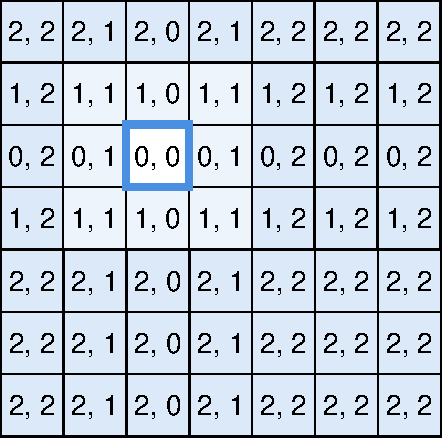
\includegraphics[width=.22\linewidth]{chap5/pos-scale.pdf}\\
	% 	\centering SI-PE
	% }	
	% \subfloat{
	% 	\centering
	% 	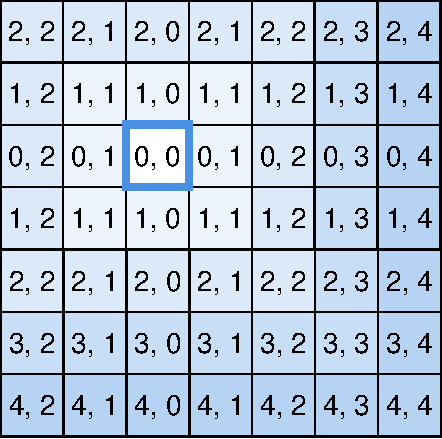
\includegraphics[width=.22\linewidth]{chap5/pos-relate.pdf}\\
	% 	\centering R-PE
	% }	
	% \subfloat{
	% 	\centering
	% 	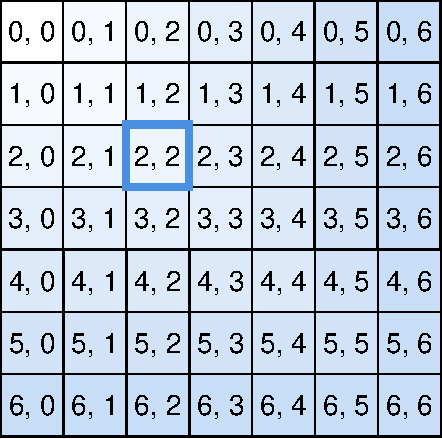
\includegraphics[width=.22\linewidth]{chap5/pos-abs.pdf}\\
	% 	\centering A-PE
	% }	
	% \subfloat{
	% 	\centering
	% 	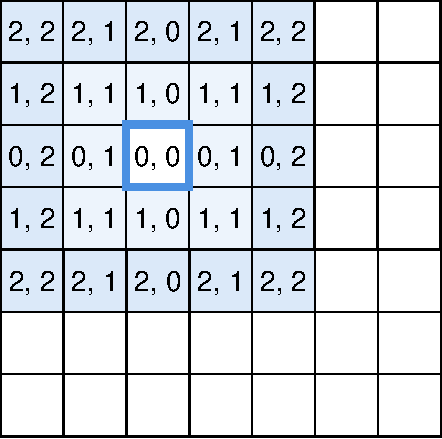
\includegraphics[width=.22\linewidth]{chap5/pos-local.pdf}\\
	% 	\centering LR-PE
	% }
	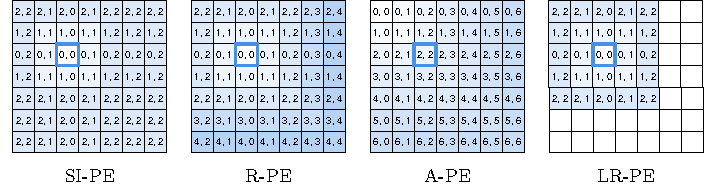
\includegraphics[width = 1\columnwidth]{chap5/pos_enc.pdf}
	\bicaption{不同的位置编码示意图。蓝色方框表示查询点的位置。每个特征点上的有序数对表示(行偏移,列偏移)。SI-PE:尺度不敏感位置编码;R-PE:相对位置编码;A-PE:绝对位置编码;LR-PE:局部相对位置编码}{The illustration of different positional encoding methods. The blue rectangle indicates the position of query. The ordered pair in each feature point is (row offset, column offset). SI-PE: scale-insensitive positional encoding; R-PE: relative positional encoding; A-PE: absolute positional encoding; LR-PE: local relative positional encoding}
	\label{fig5:PE}
\end{figure}

\subsubsection{尺度不敏感位置编码}
Vaswani等人\cite{vaswani2017attention}在自然语言处理任务中将位置编码引入Transformer以提升其性能。Transformer-xl \cite{dai2019transformer} 进一步将绝对位置编码扩展到相对位置编码。直觉上,我们可以将编码分为行编码和列编码,以将一维的相对或绝对位置编码扩展为用于图像抠图的二维位置编码。但是,已有的位置编码方式的严重的问题是注意力机制中的邻域大小必须固定。一旦输入图像的尺寸大于训练图像的尺寸,就会有一些在训练中从未出现过的位置编码,这使得测试过程变得不可行。在图像抠图中,测试图像大于训练所用图像区块的情况是非常常见的。为解决这个问题,我们为全局HOP模块提出了对尺度变化不敏感的位置编码。

在所提出的尺度不敏感位置编码中,定义空间近邻半径$s$。任意点超出半径的特征点共享完全相同的位置编码,而在半径$s$的特征点则采用相对位置编码。则带有该位置编码的全局HOP模块可以写为
\begin{equation}
\begin{aligned}
e_d =& \begin{cases} W_{PE}\,r_d  \quad d\le s;\\ W_{PE}\,r_s   \quad otherwise,\end{cases} \\
a_{(i,j),(x,y)} =& \mathop{\mathrm{softmax}}_{(x,y)}(\frac{q_{(i,j)}^Tk_{(x,y)}}{\|q_{(i,j)}\|\|k_{(x,y)}\|}\\ & + \frac{q_{(i,j)}^T}{\|q_{(i,j)}\|}(e_{|i-x|}+e_{|j-y|})),\\
g_{(i,j)} =& W_{out}(\sum_{(x,y)}a_{(i,j),(x,y)}f^O_{(x,y)}) + f^O_{(i,j)},
\end{aligned}
\end{equation}
式中我们延续文献\parencite{vaswani2017attention,dai2019transformer}的设定采用正弦编码,并在实现中采用$s=7$。借助尺度不敏感位置编码,所提出的HOP Matting方法能够处理任意形状和尺度的输入图像。除位置编码外,我们还设计了trimap图编码,以学习在注意力机制中是否需要给前景、背景和位置区域设置不同的权重。因此$(e_{|i-x|}+e_{|j-y|})$项可以被改进为$(e_{|i-x|}+e_{|j-y|}+W_{T}t_{(x,y)})$,其中$t_{x,y}$是在缩放后的trimap图中位置$(x,y)$的数据点。

\subsubsection{局部相对位置编码}
对于局部HOP模块,邻域大小在网络中始终是一个常数,这使得其并不需要尺度不敏感位置编码。
我们将文献\parencite{ramachandran2019stand}中提出的局部相对位置编码扩展为具有方向不变性(direction-invariant)的版本,而没有提出新的编码方式。局部HOP模块中的位置编码方式如图\ref{fig5:PE}中LR-PE所示。

与先前工作中所用的位置编码\cite{vaswani2017attention,dai2019transformer,ramachandran2019stand}形成对比,我们的图像抠图方法采用的位置编码都是具有方向不变性的,这意味着编码仅与查询和键之间的绝对距离有关,而和两者之间相对的方向位置无关。这种特性源自于自然图像抠图属于语义层次较低的低级视觉问题,所以应该具有旋转不变性(rotation-invariant)。

\subsection{神经网络实现细节}

在该网络模型的训练中,我们依然延续了基线网络模型的训练设定。损失函数采用了公式(\ref{eq5:loss})中的alpha预测损失,仅在trimap图标注的位置区域对预测结果和真实标注计算平均L1损失。对于不透明度编码器,我们使用了在ImageNet数据集\cite{russakovsky2015imagenet}上预训练的ResNet-34网络\cite{he2016deep}的前11个模块。而对于图像外观编码器,我们只选择了步长为2的卷积层进行堆叠,以抽取尽可能低级的图像特征。
网络模型使用Adobe Image Matting数据集\cite{xu2017deep}的前景图片和MS COCO数据集中的背景图片进行训练\cite{lin2014microsoft}。在基本数据增广部分延续了第\ref{sec5:aug}节中描述的数据增广方式,在基本增广部分之外还引入了有效的随即插值(Random Interpolation,RI)增广方式,我们将在第\ref{sec5:RI}节中对该数据增广方式及其有效性进行详细讨论。在训练时同时使用了批归一化\cite{ioffe2015batch}和谱归一化\cite{miyato2018spectral}对训练过程进行归一化操作。采用Adam优化器\cite{kingma2014adam}实现网络参数优化。同时参考文献\parencite{he2019bag},采用FP16半精度方式进行网络的训练以节约显存空间。在学习率方面,采用了学习率预热\cite{goyal2017accurate}及余弦衰减\cite{loshchilov2016sgdr}策略。




\section{实验结果}
为证明所提出方法的有效性,在本节中对所提出的两种方法进行了大量的实验,并针对HOP Matting方法设计了大量的消融实验。我们在两个被广泛使用的数据集上报告了所提出算法的评测结果:Composition-1k测试集\cite{xu2017deep}和alphamatting.com数据集\cite{rhemann2009perceptually}。在评估测度方面遵循文献\parencite{rhemann2009perceptually}的建议,采用均方误差(Mean Square Error,MSE)、总绝对差(Sum of Absolute Difference,SAD)、梯度误差(Gradient error,Grad)和连通误差(Connectivity error,Conn)对实验结果进行评估。为方便理解网络模型信息传播部分的作用,本节中将对所提两种模型的注意力机制部分进行可视化。


\begin{table}[t]
	\setlength{\tabcolsep}{15pt}
	\bicaption{使用不同测试时插值算法对Composition-1k测试集调整图片大小后的评估结果。RI表示随机插值增广}{Evaluation results on the resized Composition-1k testing set with different testing interpolations. RI is for random interpolation augmentation}
	\centering
	%    
	\begin{tabular}{l|cccc}  
		\toprule
		Methods & Test Interp.& SAD & MSE($10^{-3}$)  & Grad\\
		\midrule
		\multirow{3}{*}{ground-truth}&nearest& 21.66& 6.6& 13.76 \\
		& bilinear&5.8& 0.4&0.49 \\
		& cubic & 1.1& 0.02& 0.02\\
		\midrule
		\multirow{3}{*}{IndexNet Matting \cite{lu2019indices}}&nearest& 62.43& 23.8& 42.91 \\
		& bilinear&46.35& 14.1&24.41 \\
		& cubic & 45.65& 13.1& 25.47\\
		\midrule
		\multirow{3}{*}{HOP-5x5}&nearest&63.79&25.4&39.85\\
		& bilinear & 49.71 & 19.2 & 27.41\\
		& cubic & 38.45& 11.2  &18.87\\
		\midrule
		\multirow{3}{*}{HOP-5x5 + RI}  &nearest& 53.99 &19.5  &40.81\\
		& bilinear &30.34&6.5 &12.87\\
		& cubic & \textbf{29.42} & \textbf{6.3}&\textbf{12.16}\\
		\bottomrule
	\end{tabular}
	\label{tab5:RI}
\end{table}

\subsection{随机插值增广}
\label{sec5:RI}
经验上,深度图像抠图方法的实际性能对输入图像的缩放非常敏感。这是因为典型的自然图像抠图方法会关注图像中的细节纹理信息,而缩放操作可能会使图像边缘或高频信息出现模糊,从而导致性能下降。因此,大多数抠图方法都在原始输入图像上进行测试评估,不进行任何缩放的操作。在Context-aware Matting\cite{hou2019context}中,作者声称不同图像格式的前景和背景图片会将细微人工合成痕迹引入到合成的训练图像中,这些人工合成痕迹可以帮助网络简单地区分前景和背景。类似地,在本节中,我们将展示一些新的观察结果,即基于深度神经网络的抠图方法对不同的插值算法具有敏感性,同时对所提出的HOP Matting方法中使用的随机插值(Random Interpolation,RI)增广进行介绍。

我们在Composition-1k测试集\cite{xu2017deep}设计了一个经验性实验来支撑所描述的观察结论。首先,通过一个选定的插值算法对RGB图像进行缩放系数为1.5的上采样,然后通过相同的插值算法对放大图像进行下采样使其回到原尺寸。具体地说,假设原输入RGB图像为$800 \times 800$,并且所选的测试用插值算法为双线性插值。则通过双线性插值将输入RGB图像的大小调整为$1200 \times 1200$,然后再通过双线性插值将缩放后图像的尺寸重新调整为$800\times 800$。最后,将缩放回原尺寸的RGB图像输入网络进行alpha遮罩值预测,并评估预测值与原始真实标注之间的误差。值得注意的是,本实验并不是先进行下采样再进行上采样操作,因为先进行下采样必然会导致大量的信息丢失,而先进行上采样在理想情况下可以不产生任何信息损失。


表\ref{tab5:RI}展示了该经验性实验的评估结果。在该实验中,我们提供\textit{ground-truth}方法作为对照参考。\textit{ground-truth}方法表示直接对真实标注进行上采样和下采样,而不通过缩放后的输入图像进行任何alpha遮罩估计,然后计算缩放回原尺寸的真实标注和未经过缩放操作的真实标注之间的误差。这些结果揭示了插值操作本身所引入的误差,可以将其视为这些评估结果的理想下界。\textit{HOP-5x5}方法将作为HOP Matting方法的基本模型出现在本节的实验中。\textit{HOP-5x5}表示在局部HOP模块中采用$5\times 5$的空间邻域,并且在所有HOP模块中没有使用位置编码或trimap编码。同时我们还提供了IndexNet Matting\cite{lu2019indices}方法的评估结果作为对照。

从表\ref{tab5:RI}中可以注意到,不同测试时插值算法之间的果差距大多数结都大于\textit{ground-truth}下限之间的差距。换句话说,与插值缩放操作本身相比,作用在输入图像上的不同插值算法会在预测中引入更多误差。同时还可以看到\textit{HOP-5x5}方法的双线性插值和三次样条插值结果之间的差距大于IndexNet Matting\cite{lu2019indices}方法所给出的结果。我们对此的解释是,在训练集的数据增广中,HOP Matting方法遵循Deep Matting\cite{xu2017deep}所提出的数据合成方式,通过三次样条插值将背景图像缩放为与前景相同的大小然后合成。这种固定算法的插值增广方式使HOP Matting的模型更适合处理三次样条插值生成的数据。

基于上述经验观察结果,我们将随机插值增广方式引入所提出的HOP Matting方法。在训练阶段的数据预处理中对于任何缩放操作,都依相同的概率在不同的插值算法中进行采样,并通过采样到的插值算法实现缩放。因此,在每一个批量(mini-batch)中的合成训练图可能是由不同的插值算法生成的。此外,在合成训练图之前,可以使用不同的插值算法对前景、背景和alpha遮罩图进行缩放。如表\ref{tab5:RI}所示,使用随机插值所进行的训练不仅可以提高整体性能,而且可以减小双线性插值和三次样条插值之间误差的差距。

\begin{figure}[t]
	\centering
	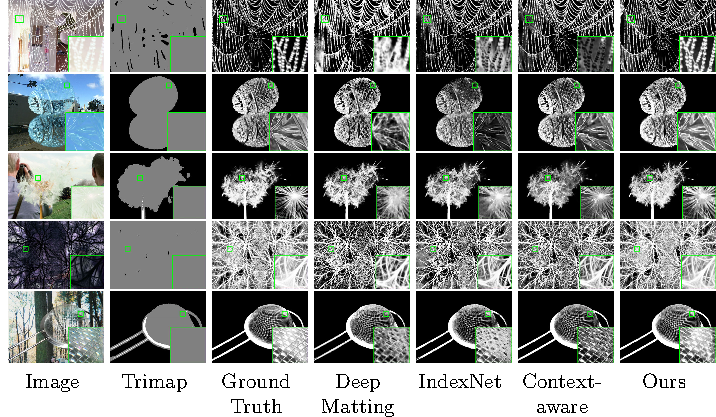
\includegraphics[width=1\textwidth]{chap5/adobe.pdf}
	\bicaption{在Composition-1k测试集\cite{xu2017deep}上的视觉效果对比结果}{The visual comparison results on Composition-1k testing set \cite{xu2017deep}}
	\label{fig5:adobe}
\end{figure}

\begin{table}[t]
	\setlength{\tabcolsep}{8pt}
	\bicaption{在Composition-1k测试集上的数值结果。PosE表示HOP模块中的位置编码,TriE表示HOP模块中的trimap编码,RI表示随机插值增广。本章所提出的不同模型变种用斜体表示,最佳数值结果加粗表示}{The quantitative results on Composition-1k testing set. PosE stands for positional encoding, and TriE is for trimap encoding in HOP blocks and RI for random interpolation augmentation. The variants of our approaches are emphasized in italic. Best results are in boldface.}
	\centering
	%    
	\begin{tabular}{l|cccc}  
		\toprule
		Methods & SAD & MSE($10^{-3}$) & Grad &Conn\\
		\midrule
		%		KNN Matting \cite{chen2013knn}& 175.4 & 103& 124.1 &176.4\\    
	%	Closed-Form Matting \cite{levin2008closed}& 168.1&91 &126.9& 167.9\\
		DCNN Matting\cite{cho2019deep}& 161.4& 87 &115.1& 161.9 \\
		Learning Based Matting \cite{zheng2009learning}&113.9& 48 &91.6 &122.2\\ 
		Information-flow Matting\cite{aksoy2017designing} & 75.4& 66& 63.0&-\\
		Deep Matting\cite{xu2017deep} &50.4& 14& 31.0& 50.8\\
		IndexNet Matting\cite{lu2019indices} &45.8&	13&	25.9&	43.7\\	
		AdaMatting\cite{cai2019disentangled}&41.7&10  &16.8 &-\\
		SampleNet Matting\cite{samplenet} &40.35&	9.9&	-&	-\\	
		Context-aware Matting\cite{hou2019context}& 35.8 & 8.2& 17.3& 33.2\\
		\midrule
		%		\textit{HOP-1x1} & 36.17& 9.1& 16.31& 33.72 \\  % & 42.53  & 40.84
		\textit{Baseline}  & 40.62 & 10.6 & 21.53 & 38.43\\
		\textit{GCA Matting} &35.28&	9.1&	16.92&	32.53\\
		\textit{HOP-5x5}& 34.82& 9.0 & 16.01& 32.04\\
		% 		\textit{HOP-5x5 + PosE}& 33.87& 8.2 & 15.34& 31.09\\
		% 		\textit{HOP-5x5 + PosE + TriE}& 34.15& 8.1 & 15.33& 31.45\\
		
		\textit{HOP-9x9}& {33.44}&{8.2}& {15.62}&{30.44} \\
		\textit{Baseline + RI}& 30.45& 6.8 & 13.23& 26.81\\
		\textit{HOP-5x5 + PosE + TriE + RI} & {28.12}& {5.8} & {11.36}& {24.13}\\
		\textit{HOP-9x9 + PosE + TriE + RI}& \textbf{27.80}& \textbf{5.7} & \textbf{11.25}& \textbf{23.73}\\
		\bottomrule
	\end{tabular}
	\label{tab5:adobe}
\end{table}
	

\subsection{Composition-1k测试集实验结果}
Composition-1k测试集\cite{xu2017deep}包含有50个不同的前景图生成的1,000张合成测试图。如表\ref{tab5:adobe}所示,本节对所提出的方法与当前最先进的自然图像抠图方法进行了定量比较。变体方法\textit{Baseline + RI}表示没有任何GCA模块或HOP模块的基线网络经过随机插值增广所训练出的网络模型。可以看出变体方法中的大多数都优于当前最先进的方法。在图\ref{fig5:adobe}中显示了Composition-1k测试集中一些测试结果的视觉效果对比。其中Deep Matting\cite{xu2017deep}的结果通过IndexNet Matting\cite{lu2019indices}中所提供的源代码和预训练模型生成。

此外,表\ref{tab5:eff}比较了一些最新方法的参数数量和模型效率。通过在具有11G显存的单个NVIDIA RTX 2080 Ti GPU上对Composition-1k测试集进行测试,该实验评估了每张测试图像的平均推理时间。值得注意的是,Context-aware Matting\cite{hou2019context}和Deep Matting\cite{xu2017deep}需要超过11G的显存或使用CPU计算,才能对Composition-1k测试集中的高分辨率图像估计其alpha遮罩值。因此,对于这两种方法,我们以缩放系数0.8对输入图像进行下采样后再进行测试。


\begin{table}[t]
	\setlength{\tabcolsep}{15pt}
	\bicaption{参数数量及使用单张NVIDIA RTX 2080 Ti显卡情况下在Composition-1k测试集上的测试效率对比。对于Deep Matting和Context-aware Matting方法,在原图基础上采用缩放系数0.8进行降采样后作为输入图片}{Parameter numbers and efficiency comparison on Composition-1k testing set on a single NVIDIA RTX 2080 Ti. Input images of Deep Matting and Context-aware Matting are downsampled with a factor of 0.8}
	\centering
	%    
	\begin{tabular}{l|cc}  
		\toprule
		Methods & \# of Parameters & Mean Time \\
		\midrule
		Deep Matting\cite{xu2017deep} &	130.6 M & 0.245 s \\
		Context-aware Matting\cite{hou2019context} & 107.5 M & 3.915 s\\
		IndexNet Matting\cite{lu2019indices} &	\textbf{6.0 M} &\textbf{ 0.182 s}\\	
		\midrule
		\textit{HOP-1x1} & 25.3 M & \textbf{0.182 s} \\
		\textit{HOP-5x5} & 25.3 M & 0.255 s \\
		\textit{HOP-9x9} & 25.3 M & 0.339 s \\
		\bottomrule
	\end{tabular}
	\label{tab5:eff}
\end{table}

\subsection{Alphamatting.com数据集实验结果}
alphamatting.com数据集被用于alphamatting在线评测排行榜,其中包含8张测试图片。每张测试图包含三种不同类型的trimap图,即小范围、大范围和用户标注。该排行榜首先对共计24个测试样例分别进行测试排名,然后再对每个类型trimap图下的8个测试样例排名取平均数,作为该类trimap图下的排名值,最后对所有测试样例的排名求取平均数,作为每个评测指标下的总排名成绩。表\ref{tab5:alphamatting}展示了所提出的两种方法在alphamatting.com排行榜中的平均排名值。每一个评估测度下的\textit{Overall}排名表示在三种类型trimap图上的所有排名名次的平均值。如表\ref{tab5:alphamatting}中排名结果所示,本章所提出的HOP Matting在不同评估测度下的表现均优于其他最先进方法,GCA Matting方法也优于多数最先进的抠图方法。

\begin{table}[t]
% \setlength{\tabcolsep}{2pt}
\bicaption{所提出两种模型在alphamatting.com排行榜上的排名得分。S、L和U分别表示排行榜测试集中三种trimap图的类型,即小范围、大范围和用户标注}{Our scores on the alphamatting.com benchmark. S, L and U denote three trimap types, small, large and user, included in the benchmark.}
\footnotesize
\centering
\begin{tabular}{@{\;\;}l|@{\;\;}c@{\;\;}|@{\;\;}c@{\;\;}c@{\;\;}c@{\;\;}|@{\;\;}c@{\;\;}|@{\;\;}c@{\;\;}c@{\;\;}c@{\;\;}|@{\;\;}c@{\;\;}|@{\;\;}c@{\;\;}c@{\;\;}c@{\;\;}}
	\toprule
	%		& \multicolumn{4}{c}{Average Rank}\\
	\multirow{2}{*}{Average Rank} & \multicolumn{4}{c@{\;\;}|@{\;\;}}{SAD}& \multicolumn{4}{c@{\;\;}|@{\;\;}}{MSE}& \multicolumn{4}{c}{Gradient Error}\\
	& Overall&S&L&U& Overall&S&L&U& Overall&S&L&U\\
	\midrule
	%mse
	HOP Matting&	\textbf{5.3}&	\textbf{5.8}	&\textbf{4}&	\textbf{6}&	\textbf{7}&	6.9&\textbf{5.4}	&8.6&\textbf{5.4}	&6.4&	\textbf{4.6}&	\textbf{5.1} \\		
	AdaMatting\cite{cai2019disentangled} &7&	6.1	&6.1&	8.8 &8&	\textbf{5.8}	&7.4&	10.8&7.6&	\textbf{4.5}&	5.3&	13\\		
	SampleNet Matting\cite{samplenet} &	7.8&5.9&	7.4&	10 &	9.1	&5.9&	9.1	&12.3&	9.1	&5.3&	6.9	&15.1\\		
	GCA Matting	&8.5&	9.3	&6.1&	10.3&9.3	&9.3&	8.3	&10.5&7.3&	7.3&	6.1&	8.5	 \\		
	Deep Matting\cite{xu2017deep}&10.1&	11.4&	9.4	&9.5&13	&11.6&	11.8&	15.6	&17.5&	14.5&	14.1&	24\\		
	Information-flow matting \cite{aksoy2017designing}&12.2&	13.3&	12.9&	10.4&13.8&	16.3&	13&	12&	20.1&	23	&18.8&	18.6\\		
	IndexNet Matting\cite{lu2019indices}&13.3&	15.5&	11.9&	12.4	&16.9&	19.4&	15.4&	15.9	&12.5&	11.4&	11&	15.3	\\		
	AlphaGAN\cite{cai2019disentangled}&14.8&	15.5&	15&	13.8&18&	18.3&	19&	16.6&17.2&	16.1&	15&	20.5\\
	Context-aware Matting\cite{hou2019context}&	17.1&	21&	15&	15.4&11.5&	14.8&	12.8	&\textbf{6.9}&8.7&	9.8&	9.4	&7	\\	
	\bottomrule
\end{tabular}
\label{tab5:alphamatting}
\end{table}


所提出的方法在大范围和用户标注两类trimap图下的评估结果明显优于绝大多数其他的最先进方法。 随着trimap图中未知区域面积变大,图像抠图也变得更加困难。因此,可以说本章所提出的方法对于未知区域面积的变化更加鲁棒。整体而言,本章所提出的自然图像抠图方法可以认为是目前此在线排行榜数据集上性能最佳的方法之一。

\subsection{消融实验}
为了验证每种成分在HOP Matting方法中的作用,本节将在Composition-1k测试集中进行三个不同的实验。
首先通过删除不同的HOP模块来对\textit{HOP-5x5}模型的效果进行评估。从表\ref{tab5:block}中报告的结果中,可以注意到层次化不透明度传播结构能够明显改善网络在图像抠图中的性能,每一个层级的HOP模块都对整体的预测效果具有明显的贡献。方法\textit{Global}\&\textit{Local Self-attention}表示将\textit{HOP-5x5}中的全局HOP模块替换为全局自注意力,并将局部HOP模块替换为局部自注意力。


\begin{table}[t]
	\setlength{\tabcolsep}{8pt}
	\bicaption{在Composition-1k测试集上对于不同HOP模块的消融实验。HOP-Local-$k$表示解码器中第$k$个局部HOP模块}{Ablation study on different HOP blocks on the Composition-1k testing set. HOP-Local-$k$ indicates the $k$-th local HOP block in the decoder.}
	\centering
	\begin{tabular}{cccc|ccc}  
		\toprule
		HOP-Global &HOP-Local-1 &HOP-Local-2 &HOP-Local-3& SAD& MSE($10^{-3}$) \\%&Grad \\% & SAD &Conn
		\midrule
		&&& & 37.89  & 10.05   \\%& 18.73\\%& 38.43
		\checkmark&&& & 36.96 & 9.89  \\%& 17.92\\%& 38.43
		\checkmark&\checkmark&&& 37.36  & 9.86 \\%& 17.77  \\% 38.73
		\checkmark&\checkmark&\checkmark& & 36.11 & 9.32 \\%& 17.23\\%  &
		\checkmark&\checkmark&\checkmark&\checkmark& \textbf{34.82} & \textbf{8.99}\\% & \textbf{16.01} \\% & 40.84   
		\midrule
		\multicolumn{4}{c|}{Global \& Local Self-attention}&  35.97 & 9.24 \\%&15.65\\
		\bottomrule
	\end{tabular}
	\label{tab5:block}
\end{table}

在第二项消融实验中,我们揭示了将位置编码、trimap编码和随机插值增广引入所提出的方法中所带来的增益效果。表\ref{tab5:emb}中提供了在Composition-1k测试集\cite{xu2017deep}评估的定量结果。可以发现,位置编码和随机插值增广的加入都会起到显著的增益效果。

为研究局部HOP模块中的邻域窗口大小如何影响所提出的方法性能,第三项消融实验在\textit{HOP-5x5}网络模型的基础上使用不同的邻域窗口大小对网络的进行了微调(fine-tune)。评估结果在表\ref{tab5:winsize}中给出。显然,更大的邻域会带来更好的测试性能。但是,如表\ref{tab5:eff}所示,局部HOP模块中较大的邻域窗口大小会导致更长的网络前馈时间,以及更多的内存消耗。



\begin{table}[t]	
	\setlength{\tabcolsep}{8pt}
	\bicaption{在Composition-1k测试集上对位置编码、trimap编码和随机插值增广的消融实验}{Ablation study on positional encoding and trimap encoding and random interpolation augmentation on the Composition-1k testing set.}
	\centering
	\begin{tabular}{l|ccc|cccc}  
		\toprule
		Method & PosE &TriE&RI& SAD& MSE($10^{-3}$) &Grad& Conn\\% & SAD &Conn
		\midrule
		\multirow{5}{*}{HOP-5x5}&&&& 34.82& 9.0 & 16.01& 32.04\\
		&\checkmark&& & 33.87& 8.2 & 15.34& 31.09\\
		&\checkmark&\checkmark&&  34.15 & 8.1 & 15.33 & 31.45\\
		&&&\checkmark & {29.01}& {6.2} & {11.93}& {25.09}\\
		&\checkmark&\checkmark&\checkmark & \textbf{28.12}& \textbf{5.8} & \textbf{11.36}& \textbf{24.13}\\
		\bottomrule
	\end{tabular}
	\label{tab5:emb}
\end{table}

\subsection{不透明度传播效果的可视化}
本节我们分别对具有单一层次不透明度传播模块的GCA Matting模型和具有多层次传播模块的HOP Matting模型中的传播效果进行可视化。

对于GCA Matting方法,本节实验通过展示具有最大注意力得分的像素位置来可视化GCA模块中所学习到的注意力图。与广泛应用于光流估计\cite{FlowNet,LiteFlowNet,PWC-Net}和图像补全\cite{yu2018generative}中,表示每个像素相对位移的偏移图(offset map)不同,此处采用的注意力图显示了在每个像素与其他像素点的相似性中具有最大相似度的相应像素的绝对位置。通过这个注意力图,可以轻松地确定每个特征像素的不透明度信息主要是从何处传播而来。如图\ref{fig5:offset}所示,在已知区域中没有信息流,已知区域都被表示为平滑连续的色域,并且未知区域中的特征区块倾向于从具有相似外观的区块中借用信息。
图\ref{fig5:offset}揭示了在输入图片上所提出的GCA模块实际关注到的的位置。
由于在从图像外观特征上抽取区块之前,GCA模块中存在用于特征对齐的卷积层,因此卷积层的参数不同导致源自两个注意力模块的注意力图并不完全相同。已知和未知部分的权重显示在注意力图的左上角。
从图\ref{fig5:offset}中的注意力偏移图中,可以轻松地识别出筛子中透出的汽车。筛子中央的浅粉红色区块表示这些特征是从汽车的左半部分中的已知区域传播来的。蓝色区块显示了从右侧和下侧道路借用来的特征。这些传播后的特征将有助于在随后的卷积层中辨别前景和背景。

\begin{table}[t]	
	\setlength{\tabcolsep}{15pt}
	\bicaption{在Composition-1k测试集上,局部HOP模块中不同的邻域窗口大小对应的数值评估结果}{The quantitative results of different neighborhood window sizes in local HOP block on the Composition-1k testing set. }
	\centering
	\small
	\begin{tabular}{c|cccc}  
		\toprule
		Neighborhood & SAD & MSE($10^{-3}$)& Grad & Conn\\% & SAD &Conn
		\midrule
		1 x 1 & 36.17& 9.1& 16.31& 33.72 \\  % & 42.53  & 40.84  
		3 x 3 & 36.02& 9.2 & 16.91& 33.59 \\  % & 42.53  & 40.84  
		5 x 5& 34.82& 9.0 & 16.01& 32.04  \\  % & 42.53  & 40.84  
		7 x 7 &34.98&8.8&16.05 & 32.37 \\  % & 42.53  & 40.84  
		9 x 9 &\textbf{33.44}&\textbf{8.2}& \textbf{15.62}&\textbf{30.44}  \\  % & 42.53  & 40.84  
		\bottomrule
	\end{tabular}
	\label{tab5:winsize}
\end{table}

对于HOP Matting方法,仅通过注意力偏移图并不能同时展示其局部与全局信息传播的层次化效果。为此,本实验通过展示输入图像上的梯度图来可视化模型所关注的像素位置。
我们从预测出的alpha遮罩值中随机选择未知区域中的一个像素点。然后,构造一个监督信息给该像素点赋予一个较大的预测损失,并假设预测出的其他alpha值完全正确的而将其他损失设为零。再后,执行反向传播,将梯度反向传播到输入图像。梯度图揭示了输入图像的每个像素与随机选择出的alpha预测像素的相关程度。我们在图\ref{fig5:vis}中显示了Composition-1k测试集\cite{xu2017deep}中测试图像及其梯度图。无HOP模块的结果是通过表\ref{tab5:block}中所训练的无HOP模块模型中生成的。
虽然由于模型中大量卷积的影响,梯度图并不像注意力偏移图一样边缘清晰。但从图\ref{fig5:vis}可以看到,具有HOP模块的模型能够在整个输入图像上聚合信息,并更加关注外观相似的区域,而没有HOP模块的模型则相反,其更多地关注所选像素点周围的局部信息。


\begin{figure}[t]
	\centering
	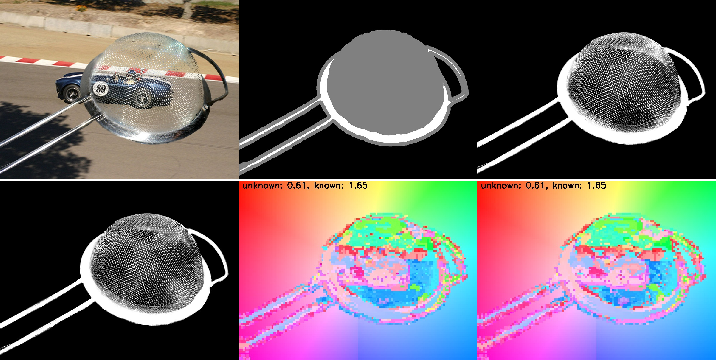
\includegraphics[width = 0.85\columnwidth]{chap5/10261offset.pdf}
	\bicaption{引导上下文注意力图的可视化。第一行从左至右分别为输入图像、trimap图和真实标注;第二行为alpha遮罩估计值、编码器中GCA模块的注意力偏移图和解码器中GCA模块的注意力偏移图}{The visualization of the guided contextual attention map. Top row from left to right, the image, trimap and ground-truth. Second row, the alpha matte prediction, attention offset map from first GCA block in the encoder, offset from GCA block in the decoder}
	\label{fig5:offset}
\end{figure}


\begin{figure}[t]
	\centering
	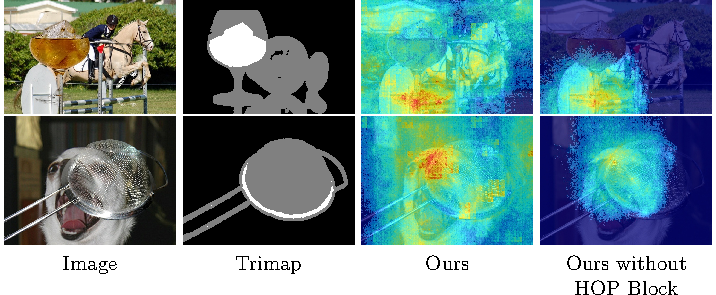
\includegraphics[width = 0.95\columnwidth]{chap5/vis.pdf}
	\bicaption{HOP结构注意力在输入图像上的可视化}{The visualization of attention in our HOP structure on input images}
	\label{fig5:vis}
\end{figure}


\section{本章小结}
在本章中,我们提出了两种基于相似性学习的端到端深度图像抠图方法。所提出的引导上下文注意力抠图方法,以全卷积的方式实现了传统基于相似性的抠图算法中的信息传播过程。其中的引导上下文注意力模块通过借助图像外观信息的引导,实现alpha特征之间的不透明度传播。而所提出的层次化不透明度传播抠图方法,则利用全局和局部模块以实现不同语义级别上的层次化信息传播。
所提出的两种方法,都通过数据驱动的训练,以网络模型的形式学习图像像素间相似性的计算方式。并依据网络模型计算出的相似性,实现不透明度信息的传播。
大量的定量实验和消融实验证明了本章所提出的抠图方法及其中的模块、数据增广方式的有效性和优越性。
% !TEX root = ../thesis.tex

\chapter{简介}

这是 \sjtuthesis 的示例文档,基本上覆盖了模板中所有格式的设置。建议大家在使用模
板之前,除了阅读《\sjtuthesis\ 使用文档》,这个示例文档也最好能看一看。

\section{二级标题}

\subsection{三级标题}

\subsubsection{四级标题}

Lorem ipsum dolor sit amet, consectetur adipiscing elit, sed do eiusmod tempor
incididunt ut labore et dolore magna aliqua. Ut enim ad minim veniam, quis
nostrud exercitation ullamco laboris nisi ut aliquip ex ea commodo consequat.
Duis aute irure dolor in reprehenderit in voluptate velit esse cillum dolore eu
fugiat nulla pariatur. Excepteur sint occaecat cupidatat non proident, sunt in
culpa qui officia deserunt mollit anim id est laborum.

\section{脚注}

Lorem ipsum dolor sit amet, consectetur adipiscing elit, sed do eiusmod tempor
incididunt ut labore et dolore magna aliqua. \footnote{Ut enim ad minim veniam,
quis nostrud exercitation ullamco laboris nisi ut aliquip ex ea commodo
consequat. Duis aute irure dolor in reprehenderit in voluptate velit esse cillum
dolore eu fugiat nulla pariatur.}

\section{字体}


上海交通大学是我国历史最悠久的高等学府之一,是教育部直属、教育部与上海市共建的全
国重点大学,是国家“七五”、“八五”重点建设和“211 工程”、“985 工程”的首批建
设高校。经过 115 年的不懈努力,上海交通大学已经成为一所“综合性、研究型、国际化”
的国内一流、国际知名大学,并正在向世界一流大学稳步迈进。 

{\songti 十九世纪末,甲午战败,民族危难。中国近代著名实业家、教育家盛宣怀和一批
  有识之士秉持“自强首在储才,储才必先兴学”的信念,于 1896 年在上海创办了交通大
  学的前身——南洋公学。建校伊始,学校即坚持“求实学,务实业”的宗旨,以培养“第
  一等人才”为教育目标,精勤进取,笃行不倦,在二十世纪二三十年代已成为国内著名的
  高等学府,被誉为“东方MIT”。抗战时期,广大师生历尽艰难,移转租界,内迁重庆,
  坚持办学,不少学生投笔从戎,浴血沙场。解放前夕,广大师生积极投身民主革命,学校
  被誉为“民主堡垒”。}

{\heiti 新中国成立初期,为配合国家经济建设的需要,学校调整出相当一部分优势专业、
  师资设备,支持国内兄弟院校的发展。五十年代中期,学校又响应国家建设大西北的号
  召,根据国务院决定,部分迁往西安,分为交通大学上海部分和西安部分。1959 年 3月
  两部分同时被列为全国重点大学,7 月经国务院批准分别独立建制,交通大学上海部分启
  用“上海交通大学”校名。历经西迁、两地办学、独立办学等变迁,为构建新中国的高等
  教育体系,促进社会主义建设做出了重要贡献。六七十年代,学校先后归属国防科工委和
  六机部领导,积极投身国防人才培养和国防科研,为“两弹一星”和国防现代化做出了
  巨大贡献。}

{\kaishu 改革开放以来,学校以“敢为天下先”的精神,大胆推进改革:率先组成教授代
  表团访问美国,率先实行校内管理体制改革,率先接受海外友人巨资捐赠等,有力地推动
  了学校的教学科研改革。1984 年,邓小平同志亲切接见了学校领导和师生代表,对学校
  的各项改革给予了充分肯定。在国家和上海市的大力支持下,学校以“上水平、创一流”
  为目标,以学科建设为龙头,先后恢复和兴建了理科、管理学科、生命学科、法学和人文
  学科等。1999 年,上海农学院并入;2005 年,与上海第二医科大学强强合并。至此,学
  校完成了综合性大学的学科布局。近年来,通过国家“985 工程”和“211 工程”的建
  设,学校高层次人才日渐汇聚,科研实力快速提升,实现了向研究型大学的转变。与此同
  时,学校通过与美国密西根大学等世界一流大学的合作办学,实施国际化战略取得重要突
  破。1985 年开始闵行校区建设,历经 20 多年,已基本建设成设施完善,环境优美的现
  代化大学校园,并已完成了办学重心向闵行校区的转移。学校现有徐汇、闵行、法华、七
  宝和重庆南路(卢湾)5 个校区,总占地面积 4840 亩。通过一系列的改革和建设,学校
  的各项办学指标大幅度上升,实现了跨越式发展,整体实力显著增强,为建设世界一流大
  学奠定了坚实的基础。}

{\fangsong 交通大学始终把人才培养作为办学的根本任务。一百多年来,学校为国家和社
  会培养了 20余万各类优秀人才,包括一批杰出的政治家、科学家、社会活动家、实业
  家、工程技术专家和医学专家,如江泽民、陆定一、丁关根、汪道涵、钱学森、吴文俊、
  徐光宪、张光斗、黄炎培、邵力子、李叔同、蔡锷、邹韬奋、陈敏章、王振义、陈竺等。
  在中国科学院、中国工程院院士中,有 200 余位交大校友;在国家 23 位“两弹一星”
  功臣中,有 6 位交大校友;在 18 位国家最高科学技术奖获得者中,有 3 位来自交大。
  交大创造了中国近现代发展史上的诸多“第一”:中国最早的内燃机、最早的电机、最早
  的中文打字机等;新中国第一艘万吨轮、第一艘核潜艇、第一艘气垫船、第一艘水翼艇、
  自主设计的第一代战斗机、第一枚运载火箭、第一颗人造卫星、第一例心脏二尖瓣分离
  术、第一例成功移植同种原位肝手术、第一例成功抢救大面积烧伤病人手术等,都凝聚着
  交大师生和校友的心血智慧。改革开放以来,一批年轻的校友已在世界各地、各行各业崭
  露头角。}

{\ifcsname lishu\endcsname\lishu\else[无 \cs{lishu} 字体。]\fi 截至 2011 年 12
  月 31 日,学校共有 24 个学院 / 直属系(另有继续教育学院、技术学院和国际教育学
  院),19 个直属单位,12 家附属医院,全日制本科生 16802 人、研究生24495 人(其
  中博士研究生 5059 人);有专任教师 2979 名,其中教授 835 名;中国科学院院士 15
  名,中国工程院院士 20 名,中组部“千人计划”49 名,“长江学者”95 名,国家杰出
  青年基金获得者 80 名,国家重点基础研究发展计划(973 计划)首席科学家 24名,国
  家重大科学研究计划首席科学家 9名,国家基金委创新研究群体 6 个,教育部创新团队
  17 个。}

{\ifcsname youyuan\endcsname\youyuan\else[无 \cs{youyuan} 字体。]\fi 学校现有本
  科专业 68 个,涵盖经济学、法学、文学、理学、工学、农学、医学、管理学和艺术等九
  个学科门类;拥有国家级教学及人才培养基地 7 个,国家级校外实践教育基地 5个,国
  家级实验教学示范中心 5 个,上海市实验教学示范中心 4 个;有国家级教学团队 8个,
  上海市教学团队 15 个;有国家级教学名师 7 人,上海市教学名师 35 人;有国家级精
  品课程 46 门,上海市精品课程 117 门;有国家级双语示范课程 7 门;2001、2005 和
  2009 年,作为第一完成单位,共获得国家级教学成果 37 项、上海市教学成果 157
  项。}

% !TeX root = ../thesis.tex

\chapter{浮动体}

\section{插图}

插图功能是利用 \TeX\ 的特定编译程序提供的机制实现的,不同的编译程序支持不同的图
形方式。有的同学可能听说“\LaTeX\ 只支持 EPS”,事实上这种说法是不准确的。\XeTeX
可以很方便地插入 EPS、PDF、PNG、JPEG 格式的图片。

一般图形都是处在浮动环境中。之所以称为浮动是指最终排版效果图形的位置不一定与源文
件中的位置对应,这也是刚使用 \LaTeX\ 同学可能遇到的问题。如果要强制固定浮动图形
的位置,请使用 \pkg{float} 宏包,它提供了 \texttt{[H]} 参数。

\subsection{单个图形}

图要有图题,研究生图题采用中英文对照,并置于图的编号之后,图的编号和图题应置于图
下方的居中位置。引用图应在图题右上角标出文献来源。当插图中组成部件由数字或字母等
编号表示时,可在插图下方添加图注进行说明,如图~\ref{fig:cn_100t} 所示。

\begin{figure}[!htp]
  \centering
  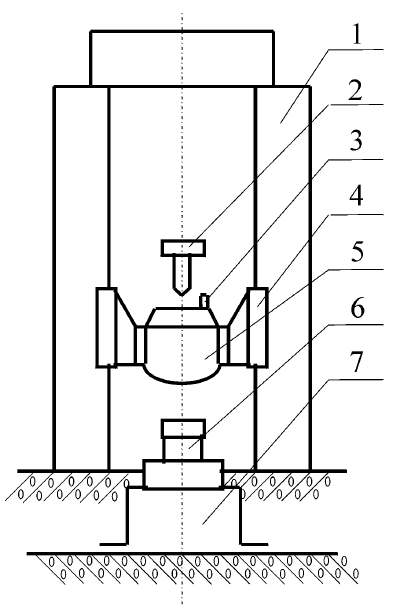
\includegraphics[width=4cm]{cn_100t.png} \\
    1.立柱 2.提升释放机构 3.标准冲击加速度计 \\
    4.导轨 5.重锤 6.被校力传感器 7.底座 \\
  \bicaption[出现在插图索引中]
    {单个图形示例\cite{he1999}。如果表格的标题很长,那么在表格索引中就会很不美观。可
      以在前面用中括号写一个简短的标题,这个标题会出现在索引中。}
    {Stay hungry, stay foolish.}
 \label{fig:cn_100t}
\end{figure}

Lorem ipsum dolor sit amet, consectetur adipisici elit, sed do eiusmod tempor
incididunt ut labore et dolore magna aliqua. Ut enim ad minim veniam, quis
nostrud exercitation ullamco laboris nisi ut aliquip ex ea commodo consequat.
Duis aute irure dolor in reprehenderit in voluptate velit esse cillum dolore eu
fugiat nulla pariatur. Excepteur sint occaecat cupidatat non proident, sunt in
culpa qui officia deserunt mollit anim id est laborum.

\subsection{多个图形}

简单插入多个图形的例子如图~\ref{fig:SRR} 所示。这两个水平并列放置的子图共用一个
图形计数器,没有各自的子图题。

\begin{figure}[!htp]
  \centering
  
\includegraphics[height=2cm]{sjtu-badge.pdf}
  \hspace{1cm}
  
\includegraphics[height=2cm]{sjtu-badge.pdf}
  \bicaption{中文题图}{English caption}
  \label{fig:SRR}
\end{figure}

如果多个图形相互独立,并不共用一个图形计数器,那么用 \texttt{minipage} 或者
\texttt{parbox} 就可以,如图~\ref{fig:parallel1} 与图~\ref{fig:parallel2}。

\begin{figure}[!htp]
\begin{minipage}{0.48\textwidth}
  \centering
  
\includegraphics[height=1.5cm]{sjtu-name.pdf}
  \caption{并排第一个图}
  \label{fig:parallel1}
\end{minipage}\hfill
\begin{minipage}{0.48\textwidth}
  \centering
  
\includegraphics[height=1.5cm]{sjtu-name.pdf}
  \caption{并排第二个图}
  \label{fig:parallel2}
\end{minipage}
\end{figure}

Lorem ipsum dolor sit amet, consectetur adipisici elit, sed do eiusmod tempor
incididunt ut labore et dolore magna aliqua. Ut enim ad minim veniam, quis
nostrud exercitation ullamco laboris nisi ut aliquip ex ea commodo consequat.
Duis aute irure dolor in reprehenderit in voluptate velit esse cillum dolore eu
fugiat nulla pariatur. Excepteur sint occaecat cupidatat non proident, sunt in
culpa qui officia deserunt mollit anim id est laborum.

如果要为共用一个计数器的多个子图添加子图题,建议使用较新的 \pkg{subcaption}宏
包,不建议使用 \pkg{subfigure} 或 \pkg{subfig} 等宏包。

推荐使用 \pkg{subcaption} 宏包的 \cs{subcaptionbox} 并排子图,子图题置于子图之
下,子图号用 a)、b) 等表示。也可以使用 \pkg{subcaption} 宏包的 \cs{subcaption}
(放在 minipage中,用法同 \cs{caption})。

搭配 \pkg{bicaption} 宏包时,可以启用 \cs{subcaptionbox} 和 \cs{subcaption} 的双
语变种 \cs{bisubcaptionbox} 和 \cs{bisubcaption},如图~\ref{fig:bisubcaptionbox}
所示。

\begin{figure}[!hbtp]
  \centering
  \bisubcaptionbox{$R_3 = 1.5\text{mm}$ 时轴承的压力分布云图}%
                  {Pressure contour of bearing when $R_3 = 1.5\text{mm}$}%
                  [6.4cm]{\includegraphics[height=2.5cm]{pressure15.jpg}}
  \hspace{1cm}
  \bisubcaptionbox{$R_3 = 2.5\text{mm}$ 时轴承的压力分布云图}%
                  {Pressure contour of bearing when $R_3 = 2.5\text{mm}$}%
                  [6.4cm]{\includegraphics[height=2.5cm]{/pressure25.jpg}}
  \bicaption{包含子图题的范例(使用 subcaptionbox)}
            {Example with subcaptionbox}
  \label{fig:bisubcaptionbox}
\end{figure}

\pkg{subcaption} 宏包也提供了 \pkg{subfigure} 和 \pkg{subtable} 环境,如
图~\ref{fig:subfigure}。

\begin{figure}[!htp]
  \centering
  \begin{subfigure}{0.3\textwidth}
    \centering
    \includegraphics[height=2cm]{sjtu-badge.pdf}
    \caption{校徽}
  \end{subfigure}
  \hspace{1cm}
  \begin{subfigure}{0.4\textwidth}
    \centering
    \includegraphics[height=1.5cm]{sjtu-name.pdf}
    \caption{校名。注意这个图略矮些,subfigure 中同一行的子图在顶端对齐。}
  \end{subfigure}
  \caption{包含子图题的范例(使用 subfigure)}
  \label{fig:subfigure}
\end{figure}

Lorem ipsum dolor sit amet, consectetur adipisici elit, sed do eiusmod tempor
incididunt ut labore et dolore magna aliqua. Ut enim ad minim veniam, quis
nostrud exercitation ullamco laboris nisi ut aliquip ex ea commodo consequat.
Duis aute irure dolor in reprehenderit in voluptate velit esse cillum dolore eu
fugiat nulla pariatur. Excepteur sint occaecat cupidatat non proident, sunt in
culpa qui officia deserunt mollit anim id est laborum.

\section{表格}

\subsection{基本表格}

编排表格应简单明了,表达一致,明晰易懂,表文呼应、内容一致。表题置于表上,研究生
学位论文可以用中、英文两种文字居中排写,中文在上,也可以只用中文。

表格的编排建议采用国际通行的三线表\footnote{三线表,以其形式简洁、功能分明、阅读
方便而在科技论文中被推荐使用。三线表通常只有 3 条线,即顶线、底线和栏目线,没有
竖线。}。三线表可以使用 \pkg{booktabs} 提供的 \cs{toprule}、\cs{midrule} 和
\cs{bottomrule}。它们与 \pkg{longtable} 能很好的配合使用。

\begin{table}[!hpt]
  \caption[一个颇为标准的三线表]{一个颇为标准的三线表\footnotemark}
  \label{tab:firstone}
  \centering
  \begin{tabular}{@{}llr@{}} \toprule
    \multicolumn{2}{c}{Item} \\ \cmidrule(r){1-2}
    Animal & Description & Price (\$)\\ \midrule
    Gnat  & per gram  & 13.65 \\
          & each      & 0.01 \\
    Gnu   & stuffed   & 92.50 \\
    Emu   & stuffed   & 33.33 \\
    Armadillo & frozen & 8.99 \\ \bottomrule
  \end{tabular}
\end{table}
\footnotetext{这个例子来自
  \href{https://mirrors.sjtug.sjtu.edu.cn/ctan/macros/latex/contrib/booktabs/booktabs.pdf}%
  {《Publication quality tables in LaTeX》}(\pkg{booktabs} 宏包的文档)。这也是
  一个在表格中使用脚注的例子,请留意与 \pkg{threeparttable} 实现的效果有何不
  同。}

\subsection{复杂表格}

我们经常会在表格下方标注数据来源,或者对表格里面的条目进行解释。可以用
\pkg{threeparttable} 实现带有脚注的表格,如表~\ref{tab:footnote}。

\begin{table}[!htpb]
  \bicaption{一个带有脚注的表格的例子}{A Table with footnotes}
  \label{tab:footnote}
  \centering
  \begin{threeparttable}[b]
     \begin{tabular}{ccd{4}cccc}
      \toprule
      \multirow{2}*{total} & \multicolumn{2}{c}{20\tnote{a}} & \multicolumn{2}{c}{40} & \multicolumn{2}{c}{60} \\
      \cmidrule(lr){2-3}\cmidrule(lr){4-5}\cmidrule(lr){6-7}
      & www & \multicolumn{1}{c}{k} & www & k & www & k \\ % 使用说明符 d 的列会自动进入数学模式,使用 \multicolumn 对文字表头做特殊处理
      \midrule
      & $\underset{(2.12)}{4.22}$ & 120.0140\tnote{b} & 333.15 & 0.0411 & 444.99 & 0.1387 \\
      & 168.6123 & 10.86 & 255.37 & 0.0353 & 376.14 & 0.1058 \\
      & 6.761    & 0.007 & 235.37 & 0.0267 & 348.66 & 0.1010 \\
      \bottomrule
    \end{tabular}
    \begin{tablenotes}
    \item [a] the first note.% or \item [a]
    \item [b] the second note.% or \item [b]
    \end{tablenotes}
  \end{threeparttable}
\end{table}

Lorem ipsum dolor sit amet, consectetur adipisici elit, sed do eiusmod tempor
incididunt ut labore et dolore magna aliqua. Ut enim ad minim veniam, quis
nostrud exercitation ullamco laboris nisi ut aliquip ex ea commodo consequat.
Duis aute irure dolor in reprehenderit in voluptate velit esse cillum dolore eu
fugiat nulla pariatur. Excepteur sint occaecat cupidatat non proident, sunt in
culpa qui officia deserunt mollit anim id est laborum.

如某个表需要转页接排,可以用 \pkg{longtable} 实现。接排时表题省略,表头应重复书
写,并在右上方写“续表 xx”,如表~\ref{tab:performance}。

\begin{longtable}[c]{c*{6}{r}}
  \bicaption{实验数据}{Experimental data}
  \label{tab:performance} \\
  \toprule
  测试程序 & \multicolumn{1}{c}{正常运行} & \multicolumn{1}{c}{同步}
    & \multicolumn{1}{c}{检查点} & \multicolumn{1}{c}{卷回恢复}
    & \multicolumn{1}{c}{进程迁移} & \multicolumn{1}{c}{检查点} \\
   & \multicolumn{1}{c}{时间 (s)} & \multicolumn{1}{c}{时间 (s)}
    & \multicolumn{1}{c}{时间 (s)} & \multicolumn{1}{c}{时间 (s)}
    & \multicolumn{1}{c}{时间 (s)} &  文件(KB)\\
  \midrule
  \endfirsthead
  \multicolumn{7}{r}{续表~\thetable} \\
  \toprule
  测试程序 & \multicolumn{1}{c}{正常运行} & \multicolumn{1}{c}{同步}
    & \multicolumn{1}{c}{检查点} & \multicolumn{1}{c}{卷回恢复}
    & \multicolumn{1}{c}{进程迁移} & \multicolumn{1}{c}{检查点} \\
   & \multicolumn{1}{c}{时间 (s)} & \multicolumn{1}{c}{时间 (s)}
    & \multicolumn{1}{c}{时间 (s)} & \multicolumn{1}{c}{时间 (s)}
    & \multicolumn{1}{c}{时间 (s)}&  文件(KB)\\
  \midrule
  \endhead
  \hline
  \multicolumn{7}{r}{续下页}
  \endfoot
  \endlastfoot
  CG.A.2 & 23.05 & 0.002 & 0.116 & 0.035 & 0.589 & 32491 \\
  CG.A.4 & 15.06 & 0.003 & 0.067 & 0.021 & 0.351 & 18211 \\
  CG.A.8 & 13.38 & 0.004 & 0.072 & 0.023 & 0.210 & 9890 \\
  CG.B.2 & 867.45 & 0.002 & 0.864 & 0.232 & 3.256 & 228562 \\
  CG.B.4 & 501.61 & 0.003 & 0.438 & 0.136 & 2.075 & 123862 \\
  CG.B.8 & 384.65 & 0.004 & 0.457 & 0.108 & 1.235 & 63777 \\
  MG.A.2 & 112.27 & 0.002 & 0.846 & 0.237 & 3.930 & 236473 \\
  MG.A.4 & 59.84 & 0.003 & 0.442 & 0.128 & 2.070 & 123875 \\
  MG.A.8 & 31.38 & 0.003 & 0.476 & 0.114 & 1.041 & 60627 \\
  MG.B.2 & 526.28 & 0.002 & 0.821 & 0.238 & 4.176 & 236635 \\
  MG.B.4 & 280.11 & 0.003 & 0.432 & 0.130 & 1.706 & 123793 \\
  MG.B.8 & 148.29 & 0.003 & 0.442 & 0.116 & 0.893 & 60600 \\
  LU.A.2 & 2116.54 & 0.002 & 0.110 & 0.030 & 0.532 & 28754 \\
  LU.A.4 & 1102.50 & 0.002 & 0.069 & 0.017 & 0.255 & 14915 \\
  LU.A.8 & 574.47 & 0.003 & 0.067 & 0.016 & 0.192 & 8655 \\
  LU.B.2 & 9712.87 & 0.002 & 0.357 & 0.104 & 1.734 & 101975 \\
  LU.B.4 & 4757.80 & 0.003 & 0.190 & 0.056 & 0.808 & 53522 \\
  LU.B.8 & 2444.05 & 0.004 & 0.222 & 0.057 & 0.548 & 30134 \\
  EP.A.2 & 123.81 & 0.002 & 0.010 & 0.003 & 0.074 & 1834 \\
  EP.A.4 & 61.92 & 0.003 & 0.011 & 0.004 & 0.073 & 1743 \\
  EP.A.8 & 31.06 & 0.004 & 0.017 & 0.005 & 0.073 & 1661 \\
  EP.B.2 & 495.49 & 0.001 & 0.009 & 0.003 & 0.196 & 2011 \\
  EP.B.4 & 247.69 & 0.002 & 0.012 & 0.004 & 0.122 & 1663 \\
  EP.B.8 & 126.74 & 0.003 & 0.017 & 0.005 & 0.083 & 1656 \\
  SP.A.2 & 123.81 & 0.002 & 0.010 & 0.003 & 0.074 & 1854 \\
  SP.A.4 & 51.92 & 0.003 & 0.011 & 0.004 & 0.073 & 1543 \\
  SP.A.8 & 31.06 & 0.004 & 0.017 & 0.005 & 0.073 & 1671 \\
  SP.B.2 & 495.49 & 0.001 & 0.009 & 0.003 & 0.196 & 2411 \\
  SP.B.4 & 247.69 & 0.002 & 0.014 & 0.006 & 0.152 & 2653 \\
  SP.B.8 & 126.74 & 0.003 & 0.017 & 0.005 & 0.082 & 1755 \\
  \bottomrule
\end{longtable}

\section{算法环境}

算法环境可以使用 \pkg{algorithms} 宏包或者较新的 \pkg{algorithm2e} 实现。
算法~\ref{algo:algorithm} 是一个使用 \pkg{algorithm2e} 的例子。关于排版算法环境
的具体方法,请阅读相关宏包的官方文档。

\begin{algorithm}[htb]
  \caption{算法示例}
  \label{algo:algorithm}
  \small
  \SetAlgoLined
  \KwData{this text}
  \KwResult{how to write algorithm with \LaTeXe }

  initialization\;
  \While{not at end of this document}{
    read current\;
    \eIf{understand}{
      go to next section\;
      current section becomes this one\;
    }{
      go back to the beginning of current section\;
    }
  }
\end{algorithm}

\section{代码环境}

我们可以在论文中插入算法,但是不建议插入大段的代码。如果确实需要插入代码,建议使
用 \pkg{listings} 宏包。

\begin{codeblock}[language=C]
#include <stdio.h>
#include <unistd.h>
#include <sys/types.h>
#include <sys/wait.h>

int main() {
  pid_t pid;

  switch ((pid = fork())) {
  case -1:
    printf("fork failed\n");
    break;
  case 0:
    /* child calls exec */
    execl("/bin/ls", "ls", "-l", (char*)0);
    printf("execl failed\n");
    break;
  default:
    /* parent uses wait to suspend execution until child finishes */
    wait((int*)0);
    printf("is completed\n");
    break;
  }

  return 0;
}
\end{codeblock}

% !TEX root = ../thesis.tex

\chapter{数学与引用文献的标注}

\section{数学}

\subsection{数字和单位}

宏包 \pkg{siunitx} 提供了更好的数字和单位支持:
\begin{itemize}
  \item \num{12345.67890}
  \item \num{1+-2i}
  \item \num{.3e45}
  \item \num{1.654 x 2.34 x 3.430}
  \item \si{kg.m.s^{-1}}
  \item \si{\micro\meter} $\si{\micro\meter}$
  \item \si{\ohm} $\si{\ohm}$
  \item \numlist{10;20}
  \item \numlist{10;20;30}
  \item \SIlist{0.13;0.67;0.80}{\milli\metre}
  \item \numrange{10}{20}
  \item \SIrange{10}{20}{\degreeCelsius}
\end{itemize}

\subsection{数学符号和公式}

微分符号 $\dif$ 应使用正体,本模板提供了 \cs{dif} 命令。除此之外,模板还提供了一
些命令方便使用:
\begin{itemize}
  \item 圆周率 $\uppi$:\verb|\uppi|
  \item 自然对数的底 $\upe$:\verb|\upe|
  \item 虚数单位 $\upi$, $\upj$:\verb|\upi| \verb|\upj|
\end{itemize}

公式应另起一行居中排版。公式后应注明编号,按章顺序编排,编号右端对齐。
\begin{equation}
  \upe^{\upi\uppi} + 1 = 0,
\end{equation}
\begin{equation}
  \frac{\dif^2 u}{\dif t^2} = \int f(x) \dif x.
\end{equation}

公式末尾是需要添加标点符号的,至于用逗号还是句号,取决于公式下面一句是接着公式说的,还是另起一句。
\begin{equation}
		\frac{2h}{\pi}\int_{0}^{\infty}\frac{\sin\left( \omega\delta \right)}{\omega}
		\cos\left( \omega x \right) \dif\omega = 
		\begin{cases}
				h, \ \left| x \right| < \delta, \\
				\frac{h}{2}, \ x = \pm \delta, \\
				0, \ \left| x \right| > \delta.
		\end{cases}
\end{equation}
公式较长时最好在等号“$=$”处转行。
\begin{align}
    & I (X_3; X_4) - I (X_3; X_4 \mid X_1) - I (X_3; X_4 \mid X_2) \nonumber \\
  = & [I (X_3; X_4) - I (X_3; X_4 \mid X_1)] - I (X_3; X_4 \mid \tilde{X}_2) \\
  = & I (X_1; X_3; X_4) - I (X_3; X_4 \mid \tilde{X}_2).
\end{align}

如果在等号处转行难以实现,也可在 $+$、$-$、$\times$、$\div$运算符号处转行,转行
时运算符号仅书写于转行式前,不重复书写。
\begin{multline}
  \frac{1}{2} \Delta (f_{ij} f^{ij}) =
    2 \left(\sum_{i<j} \chi_{ij}(\sigma_{i} - \sigma_{j})^{2}
    + f^{ij} \nabla_{j} \nabla_{i} (\Delta f) \right. \\
  \left. + \nabla_{k} f_{ij} \nabla^{k} f^{ij} +
    f^{ij} f^{k} \left[2\nabla_{i}R_{jk}
    - \nabla_{k} R_{ij} \right] \vphantom{\sum_{i<j}} \right).
\end{multline}

\subsection{定理环境}

示例文件中使用 \pkg{ntheorem} 宏包配置了定理、引理和证明等环境。用户也可以使用
\pkg{amsthm} 宏包。

这里举一个“定理”和“证明”的例子。
\begin{theorem}[留数定理]
\label{thm:res}
  假设 $U$ 是复平面上的一个单连通开子集,$a_1, \ldots, a_n$ 是复平面上有限个点,
  $f$ 是定义在 $U \backslash \{a_1, \ldots, a_n\}$ 上的全纯函数,如果 $\gamma$
  是一条把 $a_1, \ldots, a_n$ 包围起来的可求长曲线,但不经过任何一个 $a_k$,并且
  其起点与终点重合,那么:

  \begin{equation}
    \label{eq:res}
    \ointop_\gamma f(z)\, \dif z = 2\uppi \upi \sum_{k=1}^n \operatorname{I}(\gamma, a_k) \operatorname{Res}(f, a_k).
  \end{equation}

  如果 $\gamma$ 是若尔当曲线,那么 $\operatorname{I}(\gamma, a_k) = 1$,因此:

  \begin{equation}
    \label{eq:resthm}
    \ointop_\gamma f(z)\, \dif z = 2\uppi \upi \sum_{k=1}^n \operatorname{Res}(f, a_k).
  \end{equation}

  在这里,$\operatorname{Res}(f, a_k)$ 表示 $f$ 在点 $a_k$ 的留数,
  $\operatorname{I}(\gamma, a_k)$ 表示 $\gamma$ 关于点 $a_k$ 的卷绕数。卷绕数是
  一个整数,它描述了曲线 $\gamma$ 绕过点 $a_k$ 的次数。如果 $\gamma$ 依逆时针方
  向绕着 $a_k$ 移动,卷绕数就是一个正数,如果 $\gamma$ 根本不绕过 $a_k$,卷绕数
  就是零。

  定理~\ref{thm:res} 的证明。

  \begin{proof}
    首先,由……

    其次,……

    所以……
  \end{proof}
\end{theorem}

\section{引用文献的标注}

按照教务处的要求,参考文献外观应符合国标 GB/T 7714 的要求。模版使用 \BibLaTeX\
配合 \pkg{biblatex-gb7714-2015} 样式包
\footnote{\url{https://www.ctan.org/pkg/biblatex-gb7714-2015}}
控制参考文献的输出样式,后端采用 \pkg{biber} 管理文献。

请注意 \pkg{biblatex-gb7714-2015} 宏包 2016 年 9 月才加入 CTAN,如果你使用的
\TeX\ 系统版本较旧,可能没有包含 \pkg{biblatex-gb7714-2015} 宏包,需要手动安装。
\BibLaTeX\ 与 \pkg{biblatex-gb7714-2015} 目前在活跃地更新,为避免一些兼容性问
题,推荐使用较新的版本。

正文中引用参考文献时,使用 \verb|\cite{key1,key2,key3...}| 可以产生“上标引用的
参考文献”,如 \cite{Meta_CN,chen2007act,DPMG}。使用
\verb|\parencite{key1,key2,key3...}| 则可以产生水平引用的参考文献,例如
\parencite{JohnD,zhubajie,IEEE-1363}。请看下面的例子,将会穿插使用水平的和上标的
参考文献:关于书的\parencite{Meta_CN,JohnD,IEEE-1363},关于期刊的
\cite{chen2007act,chen2007ewi},会议论文 \parencite{DPMG,kocher99,cnproceed},硕
士学位论文\parencite{zhubajie,metamori2004},博士学位论文
\cite{shaheshang,FistSystem01,bai2008},标准文件 \parencite{IEEE-1363},技术报告
\cite{NPB2},电子文献 \parencite{xiaoyu2001, CHRISTINE1998},用户手册
\parencite{RManual}。

当需要将参考文献条目加入到文献表中但又不在正文中引用,可以使用
\verb|\nocite{key1,key2,key3...}|。使用 \verb|\nocite{*}| 可以将参考文献数据库中
的所有条目加入到文献表中。

% !TEX root = ../thesis.tex

\begin{summary}
这里是全文总结内容。

2015 年 2 月 28 日,中央在北京召开全国精神文明建设工作表彰暨学雷锋志愿服务大会,
公布全国文明城市(区)、文明村镇、文明单位名单。上海交通大学荣获全国文明单位称
号。

全国文明单位这一荣誉是对交大人始终高度重视文明文化工作的肯定,是对交大长期以来文
明创建工作成绩的褒奖。在学校党委、文明委的领导下,交大坚持将文明创建工作纳入学校
建设世界一流大学的工作中,全体师生医护员工群策群力、积极开拓,落实国家和上海市有
关文明创建的各项要求,以改革创新、科学发展为主线,以质量提升为目标,聚焦文明创建
工作出现的重点和难点,优化文明创建工作机制,传播学校良好形象,提升社会美誉度,显
著增强学校软实力。2007 至 2012 年间,上海交大连续三届荣获“上海市文明单位”称
号,成为创建全国文明单位的新起点。

上海交大自启动争创全国文明单位工作以来,凝魂聚气、改革创新,积极培育和践行社会主
义核心价值观。坚持统筹兼顾、多措并举,将争创全国文明单位与学校各项中心工作紧密结
合,着力构建学校文明创建新格局,不断提升师生医护员工文明素养,以“冲击世界一流大
学汇聚强大精神动力”为指导思想,以“聚焦改革、多元推进、以评促建、丰富内涵、彰显
特色”为工作原则,并由全体校领导群策领衔“党的建设深化、思想教育深入、办学成绩显
著、大学文化丰富、校园环境优化、社会责任担当”六大板块共 28 项重点突破工作,全面
展现近年来交大文明创建工作的全貌和成就。

进入新阶段,学校将继续开拓文明创建工作新格局,不断深化工作理念和工作实践,创新工
作载体、丰富活动内涵、凸显创建成效,积极服务于学校各项中心工作和改革发展的大局
面,在上级党委、文明委的关心下,在学校党委的直接领导下,与时俱进、开拓创新,为深
化内涵建设、加快建成世界一流大学、推动国家进步和社会发展而努力奋斗!

上海交通大学医学院附属仁济医院也获得全国文明单位称号。
\end{summary}


% 使用英文字母对附录编号
\appendix

% 附录内容,本科学位论文可以用翻译的文献替代。
% !TEX root = ../thesis.tex

\chapter{Maxwell Equations}

选择二维情况,有如下的偏振矢量:
\begin{subequations}
  \begin{align}
    {\bf E} &= E_z(r, \theta) \hat{\bf z}, \\
    {\bf H} &= H_r(r, \theta) \hat{\bf r} + H_\theta(r, \theta) \hat{\bm\theta}.
  \end{align}
\end{subequations}
对上式求旋度:
\begin{subequations}
  \begin{align}
    \nabla \times {\bf E} &= \frac{1}{r} \frac{\partial E_z}{\partial\theta}
      \hat{\bf r} - \frac{\partial E_z}{\partial r} \hat{\bm\theta}, \\
    \nabla \times {\bf H} &= \left[\frac{1}{r} \frac{\partial}{\partial r}
      (r H_\theta) - \frac{1}{r} \frac{\partial H_r}{\partial\theta} \right]
      \hat{\bf z}.
  \end{align}
\end{subequations}
因为在柱坐标系下,$\overline{\overline\mu}$ 是对角的,所以 Maxwell 方程组中电场
$\bf E$ 的旋度:
\begin{subequations}
  \begin{align}
    & \nabla \times {\bf E} = \upi \omega {\bf B}, \\
    & \frac{1}{r} \frac{\partial E_z}{\partial\theta} \hat{\bf r} -
      \frac{\partial E_z}{\partial r}\hat{\bm\theta} = \upi \omega \mu_r H_r
      \hat{\bf r} + \upi \omega \mu_\theta H_\theta \hat{\bm\theta}.
  \end{align}
\end{subequations}
所以 $\bf H$ 的各个分量可以写为:
\begin{subequations}
  \begin{align}
    H_r &= \frac{1}{\upi \omega \mu_r} \frac{1}{r}
      \frac{\partial E_z}{\partial\theta}, \\
    H_\theta &= -\frac{1}{\upi \omega \mu_\theta}
      \frac{\partial E_z}{\partial r}.
  \end{align}
\end{subequations}
同样地,在柱坐标系下,$\overline{\overline\epsilon}$ 是对角的,所以 Maxwell 方程
组中磁场 $\bf H$ 的旋度:
\begin{subequations}
  \begin{align}
    & \nabla \times {\bf H} = -\upi \omega {\bf D}, \\
    & \left[\frac{1}{r} \frac{\partial}{\partial r}(r H_\theta) - \frac{1}{r}
      \frac{\partial H_r}{\partial\theta} \right] \hat{\bf z} = -\upi \omega
      {\overline{\overline\epsilon}} {\bf E} = -\upi \omega \epsilon_z E_z
      \hat{\bf z}, \\
    & \frac{1}{r} \frac{\partial}{\partial r}(r H_\theta) - \frac{1}{r}
      \frac{\partial H_r}{\partial\theta} = -\upi \omega \epsilon_z E_z.
  \end{align}
\end{subequations}
由此我们可以得到关于 $E_z$ 的波函数方程:
\begin{equation}
  \frac{1}{\mu_\theta \epsilon_z} \frac{1}{r} \frac{\partial}{\partial r}
  \left(r \frac{\partial E_z}{\partial r} \right) + \frac{1}{\mu_r \epsilon_z}
  \frac{1}{r^2} \frac{\partial^2E_z}{\partial\theta^2} +\omega^2 E_z = 0.
\end{equation}

% !TEX root = ../thesis.tex

\chapter{绘制流程图}

图~\ref{fig:flow_chart} 是一张流程图示意。使用 \pkg{tikz} 环境,搭配四种预定义节
点(\verb+startstop+、\verb+process+、\verb+decision+和\verb+io+),可以容易地绘
制出流程图。

\begin{figure}[!htp]
  \centering
  \resizebox{6cm}{!}{\begin{tikzpicture}[node distance=2cm]
    \node (pic) [startstop] {待测图片};
    \node (bg) [io, below of=pic] {读取背景};
    \node (pair) [process, below of=bg] {匹配特征点对};
    \node (threshold) [decision, below of=pair, yshift=-0.5cm] {多于阈值};
    \node (clear) [decision, right of=threshold, xshift=3cm] {清晰?};
    \node (capture) [process, right of=pair, xshift=3cm, yshift=0.5cm] {重采};
    \node (matrix_p) [process, below of=threshold, yshift=-0.8cm] {透视变换矩阵};
    \node (matrix_a) [process, right of=matrix_p, xshift=3cm] {仿射变换矩阵};
    \node (reg) [process, below of=matrix_p] {图像修正};
    \node (return) [startstop, below of=reg] {配准结果};
     
    %连接具体形状
    \draw [arrow](pic) -- (bg);
    \draw [arrow](bg) -- (pair);
    \draw [arrow](pair) -- (threshold);

    \draw [arrow](threshold) -- node[anchor=south] {否} (clear);

    \draw [arrow](clear) -- node[anchor=west] {否} (capture);
    \draw [arrow](capture) |- (pic);
    \draw [arrow](clear) -- node[anchor=west] {是} (matrix_a);
    \draw [arrow](matrix_a) |- (reg);

    \draw [arrow](threshold) -- node[anchor=east] {是} (matrix_p);
    \draw [arrow](matrix_p) -- (reg);
    \draw [arrow](reg) -- (return);
\end{tikzpicture}
}
  \bicaption{绘制流程图效果}{Flow chart}
  \label{fig:flow_chart}
\end{figure}


% 文后无编号部分
\backmatter

% 参考资料
\printbibliography[heading=bibintoc]

% 用于盲审的论文需隐去致谢、发表论文、参与项目、申请专利、简历

% 致谢
% !TEX root = ../thesis.tex

%TC:ignore

\begin{acknowledgements}
  感谢那位最先制作出博士学位论文 \LaTeX 模板的交大物理系同学!

  感谢 William Wang 同学对模板移植做出的巨大贡献!

  感谢 \href{https://github.com/weijianwen}{@weijianwen} 学长一直以来的开发和维
  护工作!

  感谢 \href{https://github.com/sjtug}{@sjtug} 以及
   \href{https://github.com/dyweb}{@dyweb} 对 0.9.5 之后版本的开发和维护工作!

  感谢所有为模板贡献过代码的同学们, 以及所有测试和使用模板的各位同学!

  感谢 \LaTeX 和 \href{https://github.com/sjtug/SJTUThesis}{\sjtuthesis},帮我节
  省了不少时间。
\end{acknowledgements}

%TC:endignore


% 发表论文、参与项目、申请专利、简历
% 盲审论文中,发表学术论文及参与科研情况等仅以第几作者注明即可,不要出现作者或他人姓名
% !TEX root = ../thesis.tex

%TC:ignore

\begin{publications}
  \item {\bf{Li Y}}, Lu H. Natural Image Matting via Guided Contextual Attention. The AAAI Conference on Artificial Intelligence (AAAI). 2020. (CCF A)
  \item {\bf{Li Y}}, Zhang J, Zhao W, Weihao J, Lu H. Inductive Guided Filter: Real-time Deep Image Matting with Weakly Annotated Masks on Mobile Devices. IEEE International Conference on Multimedia and Expo (ICME). 2020  (CCF B)
  \item {\bf{Li Y}}, Lu H. On Multi-modal Fusion Learning in constraint propagation. Information Sciences. 2018 Sep 1;462:204-17. (CCF B)
  \item {\bf{Li Y}}, Chen J, Zhao Y, Lu H. Adaptive affinity matrix for unsupervised metric learning. IEEE International Conference on Multimedia and Expo (ICME). 2016 Jul 11 (pp. 1-6). IEEE. (CCF B)
  \item Zhang J, Huang Y, {\bf{Li Y}}, Zhao W, Zhang L. Multi-Attribute Transfer via Disentangled Representation. Proceedings of the AAAI Conference on Artificial Intelligence (AAAI). 2019 Jul 17 (Vol. 33, pp. 9195-9202). (CCF A)
  \item Zhang J, Niu L, Yang D, Kang L, {\bf{Li Y}}, Zhao W, Zhang L. GAIN: Gradient Augmented Inpainting Network for Irregular Holes. InProceedings of the 27th ACM International Conference on Multimedia (ACM MM). 2019 Oct 15 (pp. 1870-1878). (CCF A)
  \item Li Z, {\bf{Li Y}}, Lu H. Improve Image Captioning by Self-attention. InInternational Conference on Neural Information Processing (ICONIP). 2019 Dec 12 (pp. 91-98). Springer, Cham. (CCF C)
  \item Chen J, {\bf{Li Y}}, Lu H. Online self-organizing hashing. IEEE International Conference on Multimedia and Expo (ICME). 2016 Jul 11 (pp. 1-6). IEEE. (CCF B)
  \item Zhao Y, {\bf{Li Y}}, Shao Z, Lu H. Lsod: Local sparse orthogonal descriptor for image matching. Proceedings of the 24th ACM international conference on Multimedia (ACM MM). 2016 Oct 1 (pp. 232-236). (CCF A)
  \item Zhou M, {\bf{Li Y}}, Lu H, Nengbin C, Xuejun Z. Semi-Supervised Meta-Learning via Self-Training. In2020 3rd International Conference on Intelligent Autonomous Systems (ICoIAS) 2020 Feb 26 (pp. 1-7). IEEE.
\end{publications}

\begin{publications*}
  \item 第一作者. Natural Image Matting via Guided Contextual Attention. The AAAI Conference on Artificial Intelligence (AAAI). 2020. (CCF A)
  \item 第一作者. Inductive Guided Filter: Real-time Deep Image Matting with Weakly Annotated Masks on Mobile Devices. IEEE International Conference on Multimedia and Expo (ICME). 2020. accepted. (CCF B)
  \item 第一作者. On Multi-modal Fusion Learning in constraint propagation. Information Sciences. 2018 Sep 1;462:204-17. (CCF B)
  \item 第一作者. Adaptive affinity matrix for unsupervised metric learning. IEEE International Conference on Multimedia and Expo (ICME). 2016 Jul 11 (pp. 1-6). IEEE. (CCF B)
  \item 第三作者. Multi-Attribute Transfer via Disentangled Representation. Proceedings of the AAAI Conference on Artificial Intelligence (AAAI). 2019 Jul 17 (Vol. 33, pp. 9195-9202). (CCF A)
  \item 第五作者. GAIN: Gradient Augmented Inpainting Network for Irregular Holes. InProceedings of the 27th ACM International Conference on Multimedia (ACM MM). 2019 Oct 15 (pp. 1870-1878). (CCF A)
  \item 第二作者. Improve Image Captioning by Self-attention. InInternational Conference on Neural Information Processing (ICONIP). 2019 Dec 12 (pp. 91-98). Springer, Cham. (CCF C)
  \item 第二作者. Online self-organizing hashing. IEEE International Conference on Multimedia and Expo (ICME). 2016 Jul 11 (pp. 1-6). IEEE. (CCF B)
  \item 第二作者. Lsod: Local sparse orthogonal descriptor for image matching. Proceedings of the 24th ACM international conference on Multimedia (ACM MM). 2016 Oct 1 (pp. 232-236). (CCF A)
  \item 第二作者. Semi-Supervised Meta-Learning via Self-Training. In2020 3rd International Conference on Intelligent Autonomous Systems (ICoIAS) 2020 Feb 26 (pp. 1-7). IEEE.

\end{publications*}

%TC:endignore

% !TEX root = ../thesis.tex

%TC:ignore

\begin{projects}
  \item 参与国家自然科学基金面上项目,深度神经网络压缩及其应用研究,No. 61772330,2018年1月--2021年12月
  \item 参与Versa-上海交大联合实验室项目
\end{projects}

\begin{projects*}
\end{projects*}

%TC:endignore

% !TEX root = ../thesis.tex

%TC:ignore

\begin{patents}
  \item 第一发明人,“永动机”,专利申请号202510149890.0
\end{patents}

\begin{patents*}
  \item 第一发明人,“永动机”,专利申请号XXXXXXXXXXXX.X
\end{patents*}

%TC:endignore

% !TEX root = ../thesis.tex

%TC:ignore

\begin{resume}
  \subsection*{基本情况}
    某某,yyyy 年 mm 月生于 xxxx。

  \subsection*{教育背景}
  \begin{itemize}
    \item yyyy 年 mm 月至今,上海交通大学,博士研究生,xx 专业
    \item yyyy 年 mm 月至 yyyy 年 mm 月,上海交通大学,硕士研究生,xx 专业
    \item yyyy 年 mm 月至 yyyy 年 mm 月,上海交通大学,本科,xx 专业
  \end{itemize}

  \subsection*{研究兴趣}
    \LaTeX{} 排版

  \subsection*{联系方式}
  \begin{itemize}
    \item 地址: 上海市闵行区东川路 800 号,200240
    \item E-mail: \email{xxx@sjtu.edu.cn}
  \end{itemize}
\end{resume}

%TC:endignore


% 中文学士学位论文要求在最后有一个英文大摘要,单独编页码,英文学士学位论文不需要
% !TEX root = ../thesis.tex

\begin{bigabstract}
  An imperial edict issued in 1896 by Emperor Guangxu, established Nanyang
  Public School in Shanghai. The normal school, school of foreign studies,
  middle school and a high school were established. Sheng Xuanhuai, the person
  responsible for proposing the idea to the emperor, became the first president
  and is regarded as the founder of the university.

  During the 1930s, the university gained a reputation of nurturing top
  engineers. After the foundation of People's Republic, some faculties were
  transferred to other universities. A significant amount of its faculty were
  sent in 1956, by the national government, to Xi'an to help build up Xi'an Jiao
  Tong University in western China. Afterwards, the school was officially
  renamed Shanghai Jiao Tong University.

  Since the reform and opening up policy in China, SJTU has taken the lead in
  management reform of institutions for higher education, regaining its vigor
  and vitality with an unprecedented momentum of growth. SJTU includes five
  beautiful campuses, Xuhui, Minhang, Luwan Qibao, and Fahua, taking up an area
  of about 3,225,833 m2. A number of disciplines have been advancing towards the
  top echelon internationally, and a batch of burgeoning branches of learning
  have taken an important position domestically.

  Today SJTU has 31 schools (departments), 63 undergraduate programs, 250
  masters-degree programs, 203 Ph.D. programs, 28 post-doctorate programs, and
  11 state key laboratories and national engineering research centers.

  SJTU boasts a large number of famous scientists and professors, including 35
  academics of the Academy of Sciences and Academy of Engineering, 95 accredited
  professors and chair professors of the "Cheung Kong Scholars Program" and more
  than 2,000 professors and associate professors.

  Its total enrollment of students amounts to 35,929, of which 1,564 are
  international students. There are 16,802 undergraduates, and 17,563 masters
  and Ph.D. candidates. After more than a century of operation, Jiao Tong
  University has inherited the old tradition of "high starting points, solid
  foundation, strict requirements and extensive practice." Students from SJTU
  have won top prizes in various competitions, including ACM International
  Collegiate Programming Contest, International Mathematical Contest in Modeling
  and Electronics Design Contests. Famous alumni include Jiang Zemin, Lu Dingyi,
  Ding Guangen, Wang Daohan, Qian Xuesen, Wu Wenjun, Zou Taofen, Mao Yisheng,
  Cai Er, Huang Yanpei, Shao Lizi, Wang An and many more. More than 200 of the
  academics of the Chinese Academy of Sciences and Chinese Academy of
  Engineering are alumni of Jiao Tong University.
\end{bigabstract}


\end{document}
